\documentclass[a4paper,11pt]{report}

\usepackage[francais]{babel}
\usepackage[utf8]{inputenc}
\usepackage[T1]{fontenc}
\usepackage[pdftex]{graphicx}
\usepackage{setspace}
\usepackage{color}
\usepackage{makeidx}
\usepackage[final]{pdfpages} 
\usepackage{hyperref}
\usepackage{fancyvrb}
\usepackage{fancyhdr} %pour header
\usepackage[french]{varioref}
\usepackage [paper=a4paper,tmargin=2cm,bmargin=2.5cm,lmargin=3cm,rmargin=3cm]{geometry}
\usepackage{caption}
\usepackage{amsmath}% http://ctan.org/pkg/amsmath
\usepackage{eurosym}
%\usepackage{moreverb}
%\usepackage[Lenny]{fncychap}
%\usepackage{blkarray}
%\usepackage{verbatim}
%\usepackage{forest}

% Latex Linux packages
\usepackage{packages/moreverb}
\usepackage[Lenny]{packages/fncychap}
\usepackage{packages/blkarray}
\usepackage{packages/verbatim}
\usepackage{packages/forest}

\pagestyle{fancy}
\fancyhf{}
\renewcommand{\headrulewidth}{1pt} %barre header et foot
\renewcommand{\footrulewidth}{1pt}

\makeindex
\newcommand{\reporttitle}{\Huge{Automatisation de l'analyse d'incidents par l'utilisation du Machine Learning}}    % Titre
\newcommand{\reportauthor}{
	\Large{Florian \textsc{Lepont}}
}% Auteur
\newcommand{\reportsubject}{\huge{Stage de fin d'études}} % Sujet
\newcommand{\HRule}{\rule{\linewidth}{1.5mm}}

\setlength{\parskip}{1ex} % Espace entre les paragraphes

%entete et pied de page
\chead{Automatisation de l'analyse d'incidents}
\lfoot{Aldebaran}
\rfoot{\thepage}

\begin{document}
 \renewcommand{\contentsname}{Sommaire}  %change table des matiere en sommaire
 \begin{center}

\begin{minipage}[t]{1.1\textwidth}
  \begin{flushright}
    
\includegraphics [width=40mm,height=12mm]{images/aldebaran_logo.png} \\[0.5cm]
  \end{flushright}
\end{minipage} \\[2cm]

\textsc{\Large \reportsubject}\\[1cm]
\HRule \\[0.25cm]
\textsc{\Large \reporttitle}
{
\HRule \\[2cm]
\begin{figure}[h]
	\centering
\includegraphics[width=14cm,height=7cm]{images/main_picture.png}
\end{figure}
\bigbreak\bigbreak\bigbreak\bigbreak
\begin{minipage}[t]{0.3\textwidth}
  \begin{flushleft} \large
    \emph{\Large{Étudiant :}}\\ 
    \reportauthor
  \end{flushleft}
\end{minipage}
\begin{minipage}[ht]{0.6\textwidth}
  \begin{flushright} \large
    \emph{\Large{Tuteur entreprise :}} \\
    \Large{M.~Emmanuel \textsc{Nalepa}}
  \end{flushright}
\end{minipage}
}
\vfill

{\large 2\up{nd} semestre 2015}

\thispagestyle{empty} %pas afficher num page

\end{center}


\chapter*{Remerciements}
\thispagestyle{fancy}

Je tiens tout d'abord à remercier l'entreprise \emph{Aldebaran} de m'avoir accueilli et offert l'opportunité de réaliser mon stage ingénieur au sein de l'équipe "Qualification Hardware Pepper".

Je remercie tout particulièrement M Emmanuel Nalepa de m'avoir permis de participer à ce projet captivant et formateur, m'ayant ainsi permis d'étoffer mes connaissances dans plusieurs disciplines.  Sa disponibilité et sa pédagogie ont été des atouts essentiels à mon enrichissement technique.

J’adresse également mes remerciements aà toutes les personnes qui m’ont proposé leur aide durant ces vingt semaines :
M. Angelica Lim qui m’a fournie de précieuses informations, notamment dans le domaine du Machine Learning.

Je tiens enfin à remercier l'équipe "Qualification Hardware Pepper" pour l'aide qu'elle m'a apporté et sa très bonne humeur.

\begin{abstract}
\label{abstract}
Mon stage ingénieur, réalisé dans le cadre de ma cinquième année de formation à l'École Nationale d'Ingénieurs de Brest (ENIB), s’est déroulé au sein du département "Qualification Hadware Pepper (QWP) de l'entreprise Aldebaran. La société Parisienne s'est fait connaitre dans le monde des nouvelles technologies et de la robotique humanoïde grâce au développement de son premier produit, "Nao". A l'origine, le robot se prédestine à l'univers de la recherche et aux universités. La société cherche aujourd'hui à conquérir de nouveaux marchés en offrant des produits et des services au monde de l'entreprise et aux particuliers. Cela se traduit notamment par le développement d'un tout nouveau produit: "Pepper". 

Cette extension du marché s'accompagne d'une montée en puissance de la production des robots "Pepper". Cela induit le développement d'une nouvelle génération d'outils de production et post-production. Un des dispositif mis en place est le "Filtering Test": à la fin de la chaine de production, les robots sont soumis à une série de tests qui visent à mettre à l'épreuve les différentes parties mécaniques et électroniques. Lorsqu'une erreur est détectée,  les différentes données du robot son enregistrées (e.g. température des fusibles, valeurs de l'accéléromètre, etc.). Afin de déterminer qu'elles sont les causes qui ont entrainé l'apparition de l'anomalie sur le robot, chaque donnée est étudiée minutieusement et des hypothèses sont émises. Cette tâche dite d'investigation peu s'avérer laborieuse, le souhait d'automatiser ce processus est donc important.

Le but de  ma présence au sein d'Aldebaran est donc de répondre à ce besoin. En s'appuyant sur l'utilisation de méthodes d'apprentissage automatiques (en anglais, on parle de Machine Learning), j'ai donc mis au point un algorithme capable de déterminer automatiquement (après une phase d'apprentissage) les causes ayant entrainées l'apparition d'anomalies sur Pepper.  La mise au point de cet outil a été réalisé en trois temps:
\begin{enumerate}
	\item auto-formation à l'apprentissage automatique et de maitrise des outils.
	\item conception et développement de l'algorithme
	\item industrialisation du produit, c'est à dire en simplifier l'utilisation et le robustifier.
\end{enumerate}
 

Le rapport de stage ci-joint présente les différentes recherches effectuées ainsi que les travaux réalisés pour répondre au mieux à la problématique initiale.\end{abstract}

\tableofcontents
\listoffigures
\listoftables
\printindex
\chapter{Entreprise}
\label{Entreprise}
\thispagestyle{fancy}

\section{Histoire}
\label{Entreprise: histoire}
Aldebaran (anciennement Aldebaran Robotics) est une société française de robotique humanoïde fondée en 2005 par Bruno MAISONNIER.

\subsection{Le premier robot, NAO}
\label{Entreprise:Histoire:Nao}
Constituée au départ d'une équipe de douze collaborateurs, la toute jeune entreprise se fixe comme objectif de développer des robots humanoïdes et de les commercialiser au grand public en tant que "nouvelle espèce bienveillante à l'égard des humains". Après trois années de recherche et développement, la société dévoile en 2008 son tout premier produit: NAO. La participation du robot humanoïde à divers évènements internationaux, comme par exemple la RoboCup ou encore l'Exposition Universelle de Shanghai en 2010 participe à sa popularisation auprès des laboratoires de recherche, des universités et des développeurs. Une seconde génération de robot NAO apparait en 2011. L'entreprise dévoile durant la même période le projet Romeo dont l'objectif est de créer un véritable robot d'assistance à la personne, en partenariat avec différents acteurs de la recherche.

\subsection{La famille s'agrandit}
\label{Entreprise: La famille Aldebaran}
Lors de l'année 2012, Aldebaran Robotics est rachetée par SoftBank, société spécialisée dans le commerce électronique au Japon et prend le nom d'Aldebaran (suppression du terme "Robotics"). Débute alors la conception d'un tout nouveau produit, le robot humanoïde Pepper. Dévoilé au grand public en 2014, il est dans un premier temps vendu au Japon auprès des entreprises. Les premiers clients à en bénéficier sont les magasins de téléphonie mobile du groupe SoftBank. Les ventes s'ouvrent par la suite aux particuliers Japonais. La société compte aujourd'hui plus de 300 collaborateurs et poursuit le développement de ses trois produits afin de les améliorer et de conquérir de nouveaux marchés (Europe, Chine et États-Unis).

\section{Les produits}
\label{Entreprise: Les produits}
Aldebaran commercialise à ce jour deux produits: NAO et Pepper. Le robot Romeo est une plateforme de recherche.

\subsection{NAO}
\label{Entreprise: Les produits: Nao}
NAO est un robot humanoïde de 58 cm de hauteur. Les publics ciblés sont essentiellement les laboratoires de recherche et le monde de l'éducation (des écoles primaires jusqu'aux universités).

\begin{figure}[H]
	\centering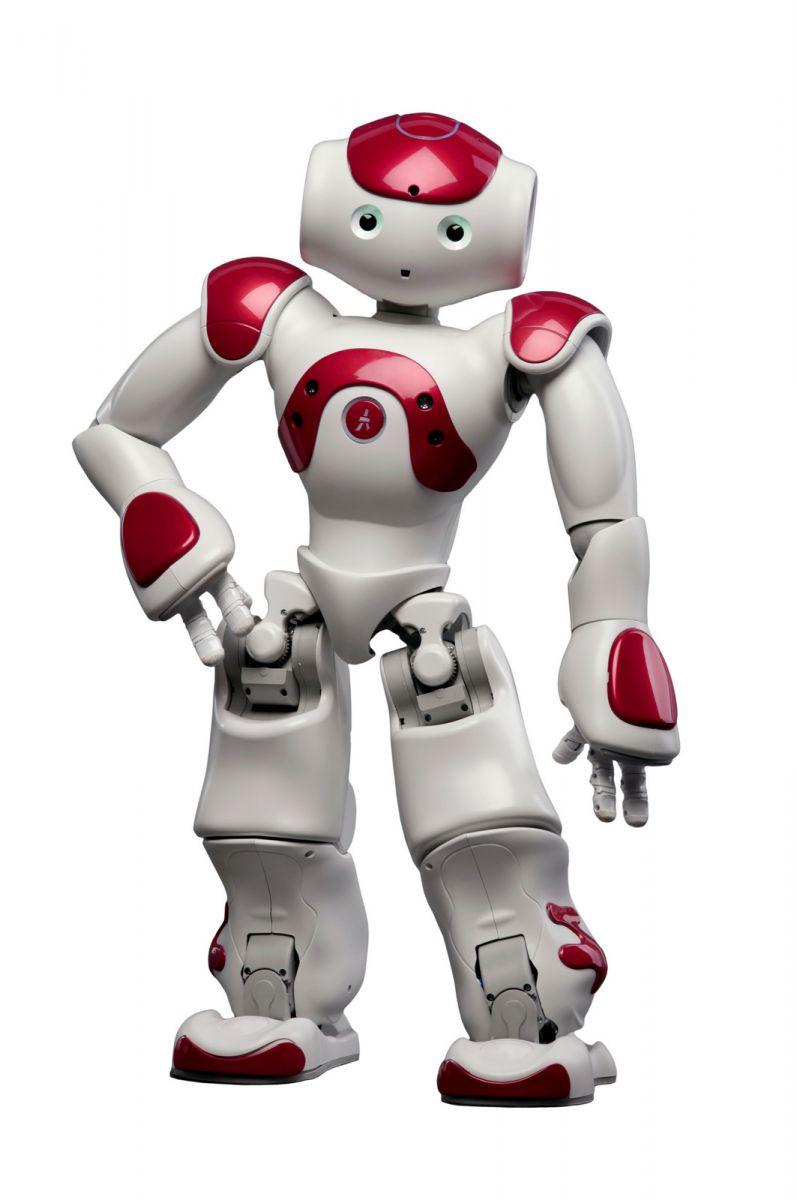
\includegraphics[height=7cm]{images/nao.jpg}
	\caption{Le robot humanoïde NAO}
	\label{fig:Robot humanoïde Nao}
\end{figure}

\paragraph{Caractéristiques techniques}
\label{Entreprise:Les produits: Nao: Caractéristiques techniques}
Caractéristiques techniques de la dernière version de Nao (V5, Évolution) tableau \ref{tab: Caractéristiques techniques de Nao}.

\begin{table}[H]
	\begin{tabular}{ | l | p{10cm} | }
	\hline
	\multicolumn{2}{|c|}{Caractéristiques générales} \\
	\hline
	Dimensions & 574 x 311 x 275 mm \\
	\hline 
	Masse & 5.4 kg \\
	\hline 
	Degrés de liberté  & 25 \\
	\hline
	Processeur & Intel Atom Z530 \newline 1.6 GHz \newline RAM: 1GB \newline Mémoire flash: 2GB  \newline Micro SDHC: 8 GB \\
	\hline
	Système d'exploitation & Middleware Aldebaran NAOqi basé sur un noyau Linux \\
	\hline
	Connectivité & Wi-Fi, Ethernet, USB \\
	\hline
	Batterie & Autonomie: 90 minutes en usage normal \newline Energie: 48.6 Wh \\
	\hline 
	Vision & Deux caméras frontales 2D, 1220p, 30ips \\
	\hline
	Audio & Sortie: 2 haut-parleurs stéréo \newline 4 microphones directionnels \newline moteur de reconnaissance vocale Nuance  \\
	\hline
	Capteurs & 2 capteurs infra-rouges, résistance sensible à la pression, centrale inertielle, 2 systèmes sonars, 3 surfaces tactiles \\
	\hline
	\end{tabular}
\caption[Caractéristiques techniques de NAO]{Caractéristiques techniques de la dernière version commerciale de NAO}
\label {tab: Caractéristiques techniques de Nao}
\cite{NaoTech}
\end{table}

\subsection{Pepper}
\label{Entreprise: Les produits: Pepper}
Dernier né d'Aldebaran, le robot Pepper est conçu pour vivre au côté des humains. Imaginé au départ pour accompagner et informer les clients dans les magasins de téléphonie du groupe japonais SoftBank, l'entreprise cherche à présent à placer son produit chez les particuliers. Le robot reprend la structure software et hardware de NAO. Contrairement à ce dernier, Pepper se déplace non pas grâce à une paire de jambes, mais via trois roues omnidirectionnelles qui facilitent son déplacement. A noter également que celui-ci est équipé d'une tablette tactile sur son torse pour faciliter les interactions Homme-Machine.

\begin{figure}[H]
	\centering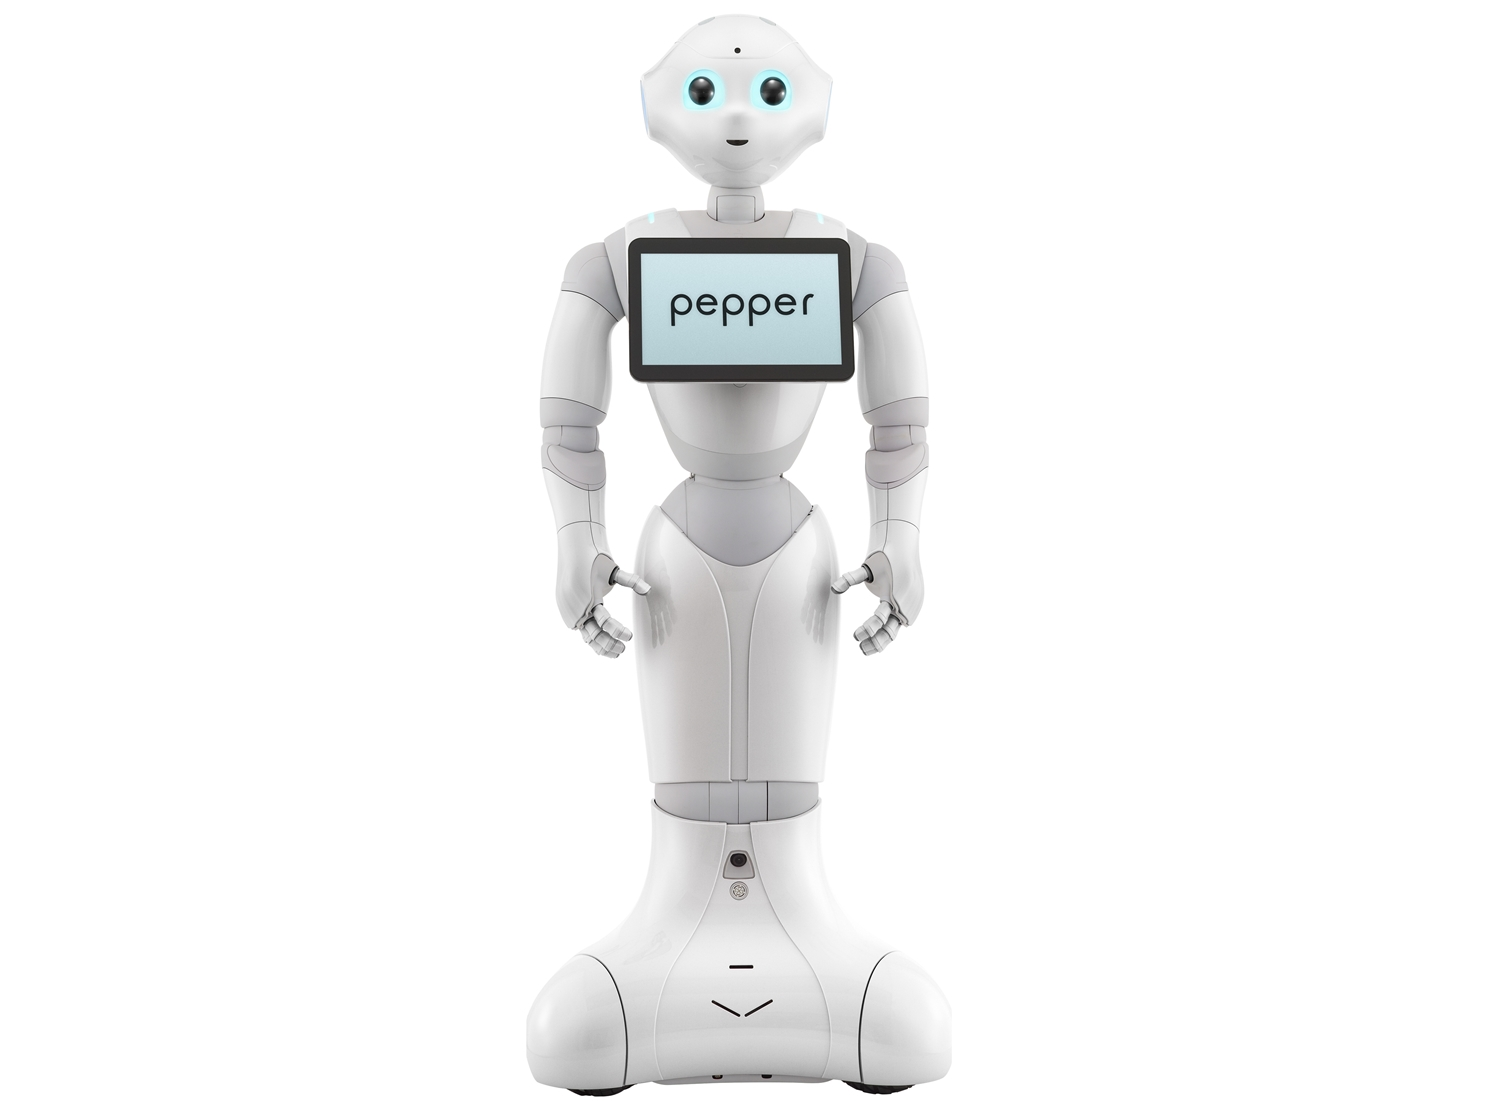
\includegraphics[height=6cm]{images/pepper.jpg}
	\caption{Le robot humanoïde Pepper}
	\label{fig:Robot humanoïde Pepper}
\end{figure}

\paragraph{Caractéristiques techniques}
Caractéristiques techniques de la dernière version commerciale de Pepper (V1.7) tableau \ref{tab: Caractéristiques techniques de Pepper}.

\begin{table}[H]
\begin{tabular}{ | l | p{10cm} | }
	\hline
	\multicolumn{2}{|c|}{Caractéristiques générales} \\
	\hline
	Dimensions & 1210 x 480 x 425 mm \\
	\hline 
	Masse & 28 kg \\
	\hline 
	Degrés de liberté  & 20 \\
	\hline
	Processeur & Intel Atom E3845 \newline 1.91 GHz \newline RAM: 4 GB \newline Mémoire flash: 8 GB \newline MICRO SDHC: 16Go  \\
	\hline
	Système d'exploitation & Middleware Aldebaran NAOqi,\newline basé sur un noyau Linux \\
	\hline
	Connectivité & Wi-Fi, Ethernet, USB \\
	\hline
	Batterie & Énergie: 795 Wh \\
	\hline 
	Vision & 2 caméras 2D \newline 1 caméra 3D \\
	\hline
	Audio & 3 microphones directionnels \newline moteur de reconnaissance vocale Nuance  \\
	\hline
	Connectivité & Wi-Fi, Ethernet \\
	\hline
	Capteurs & 6 lasers, 2 capteurs infra-rouges, 1 système sonar, résistance sensible à la pression, 2 centrales inertielles, 3 surfaces tactiles \\
	\hline
\end{tabular}
\caption[Caractéristiques techniques de Pepper]{Caractéristiques techniques de la dernière version commerciale  de Pepper}
\label {tab: Caractéristiques techniques de Pepper}
\cite{PepperTech}
\end{table}

\subsection{Romeo}
\label{Entreprise: Les produits: Romeo}
Romeo est un nouveau type de robot d'accompagnement et d'assistance à la personne. Cette plateforme de recherche est soutenue par Aldebaran ainsi que d'autres partenaires universitaires et laboratoires de recherche (e.g. INRIA, LAAS-CNRS, ISIR, ENSTA, Telecom, etc.). Il s'agit pour l'instant d'un prototype et sert principalement de plateforme de tests pour les prochaines innovations majeures d'Aldebaran (e.g. yeux mobiles, système vestibulaire, etc.).

\begin{figure}[H]
	\centering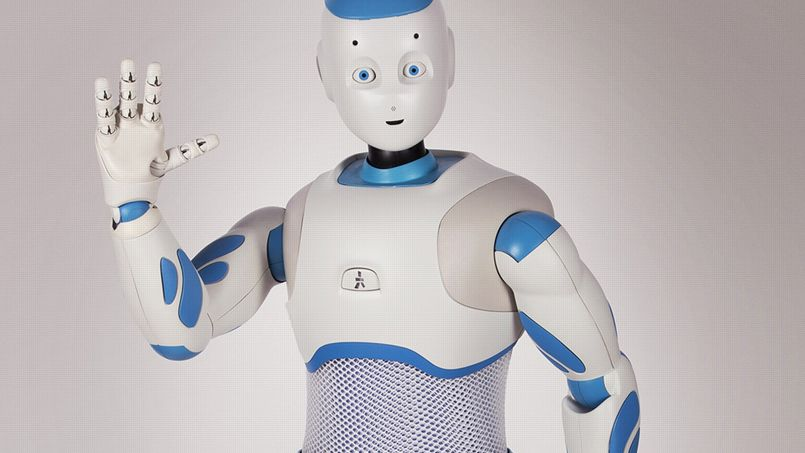
\includegraphics[height=6cm]{images/romeo.jpg}
	\caption{Le robot humanoïde Romeo}
	\label{fig:Robot humanoïde Romeo}
\end{figure}

\paragraph{Caractéristiques techniques}
Caractéristiques techniques de la dernière version commerciale de Romeo (V2) tableau \ref{tab: Caractéristiques techniques de Romeo}.

\begin{table}[H]
	\begin{tabular}{ | l | p{10cm} | }
		\hline
		\multicolumn{2}{|c|}{Caractéristiques générales} \\
		\hline
		Hauteur & 1467 mm \\
		\hline 
		Masse & 37 kg \\
		\hline
		Processeur & Intel ATOM Z530 \newline 1.6 GHz \newline RAM: 1 GB \newline Mémoire flash: 2 GB \newline MICRO SDHC: 8 Go  \\
		\hline
		Système d'exploitation & Middleware Aldebaran NAOqi,\newline basé sur un noyau Linux \\
		\hline
		Connectivité & Wi-Fi, Ethernet \\
		\hline
		Batterie & Énergie: 795 Wh \\
		\hline 
		Vision & 4 caméras 2D \newline 1 caméra 3D \\
		\hline
		Audio & 3 microphones directionnels \newline moteur de reconnaissance vocale Nuance  \\
		\hline
		Connectivité & Wi-Fi, Ethernet \\
		\hline
		Capteurs & 6 lasers, 2 capteurs infra-rouges, 1 système sonar, résistance sensible à la pression, 2 centrales inertielles, 3 surfaces tactiles \\
		\hline
	\end{tabular}
	\caption[Caractéristiques techniques de Romeo]{Caractéristiques techniques de la dernière version de Romeo}
	\label {tab: Caractéristiques techniques de Romeo}
	\cite{RomeoTech}
\end{table}

\subsection{Le système d'exploitation NAOqi}
\label{Entreprise: Les produits: NAOqi}
NAOqi est le système d'exploitation commun aux 3 robots d'Aldebaran. Il se base sur la distribution de Linux Gentoo et contient plusieurs APIs qui permettent de commander et contrôler les robots \cite{NAOqiTech}.
\begin{description}
	\item [NAOqi Core:] Gestion de l'ensemble des fonctions de base des robots (e.g. mémoire, "Autonomous Life", comportement du robot, etc.).
	\item [NAOqi Motion:] Gestion des mouvements du robot.
	\item [NAOqi Audio:]  Gestion de la partie audio du robot.
	\item [NAOqi Vision:] Gestion de la partie vidéo du robot.
	\item [NAOqi People Perception:] Ce module est utilisé pour détecter la présence de personnes autour du robot.
	\item [NAOqi Sensors:]  Gestion de l'ensemble des capteurs qui équipent le robot.
\end{description} 


\subsection{Plateforme de développement}
\label{Entreprise:Les produits: Nao: Plateforme de développement}
Les robots sont fournis avec une plateforme de développement.
\begin{description}
	\item[Choregraphe:] Il s'agit d'un outil de programmation graphique basé sur une interface qui prend la forme de schémas blocs \cite{ChoregrapheTech}. Il permet de façon simple d'interagir avec le robot et de concevoir des applications . Il peut s'utiliser avec un environnement de simulation 3D permettant aux développeurs de tester leurs applications sans même posséder un robot. Le logiciel permet également de disposer d'un retour visuel sur ce que le robot perçoit (e.g. vidéos issues des caméras, données des moteurs, etc.)
	
	\item[Kit de développement (SDK):] Il permet de développer des applications pour les robots via plusieurs langages de programmation:  C++, Python et Java \cite{SDKTech}.
\end{description}


\chapter{Introduction}
\label{Introduction}
\thispagestyle{fancy}

\section{Présentation du produit}
\label{Introduction:Présentation du produit}
On présente ici de manière succincte l'architecture Hardware du robot Pepper afin de se familiariser avec les différents éléments du système avec lesquels on sera susceptible de travailler durant la mise en œuvre de ce projet.  

\subsection{Les actionneurs}
\label{Introduction:Présentation du produit:Les actionneurs}
\subsubsection{Les moteurs}
\label{Introduction:Présentation du produit:Les actionneurs: Les moteurs}
Le robot Pepper est constitué de 20 moteurs dont il est possible de contrôler la position et la rigidité (figure \ref{fig:Répartition des actionneurs de Pepper})
\begin{description}
	\item [Tête:] 2 moteurs pour les mouvements de lacet (HeadYaw) et de tangage (HeadPitch)
	\item [Bras:] 4 moteurs par bras, répartis de la manière suivante: 
	\begin{description}
		\item [Épaule:] 2 moteurs pour les mouvements de tangage (ShoulderPitch) et de roulis du bras (ShoulderRoll).
		\item [Coude:] 2 moteurs pour les mouvements de roulis (ElbowRoll) et de lacet (ElbowYaw) de l'avant-bras.
	\end{description}
	\item [Main:] 1 moteur pour le mouvement de lacet du poignet (WristYaw) et 1 pour le mouvement d'ouverture et de fermeture de la main (Hand).
	\item [Hanche:] 2 moteurs pour le mouvement de roulis (HipRoll) et de tangage (HipPitch) du buste.
	\item [Genoux:] 1 moteur pour le mouvement de tangage (KneePitch) du haut du corps.
	\item [Roues:] 3 moteurs pour les mouvements de rotation de chacune des 3 roues omnidirectionnelles (WheelB, WheelFR et WheelFL).
\end{description}

\begin{figure}[h]
	\centering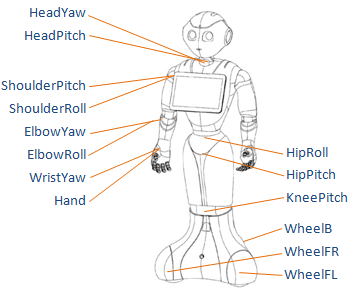
\includegraphics[height=7cm]{images/pepper_motors.png}
	\caption{Répartition des actionneurs de Pepper}
	\label{fig:Répartition des actionneurs de Pepper}
\end{figure}

\subsubsection{Les LEDs}
\label{Introduction:Présentation du produit:Les actionneurs: Les leds}
Les LEDs placées sur les épaules de Pepper, autour de ses yeux et de ses oreilles permettent d'obtenir un certain nombre d'informations sur son état. Par exemple, des LEDs bleues en rotations autour des yeux indiquent que le robot écoute.

\subsection{Les capteurs}
\label{Introduction:Présentation du produit:Les capteurs}
Pepper intègre également une multitude de capteurs. Certains d'entre eux sont utilisés pour s'assurer du bon comportement des parties mécaniques du robot, ou pour réaliser du contrôle-commande. D'autres capteurs sont en revanche intégrés sur le robot afin que l'utilisateur puisse interagir avec lui (tableau \ref{tab: Les différents capteurs de Pepper}).

\begin{table}[h]
	\begin{tabular}{ | p{3cm} | p{4cm} | p{7cm} | }
		\hline
		Capteur & Position & Description \\
		\hline
		Capteurs liés aux actionneurs & sur les moteurs & Chaque moteur du robot est lié à 3 capteurs, qui donnent des informations sur la valeur du courant délivré au moteur (A), la température du moteur (\degres C) et la position du moteur. \\
		\hline
		Capteurs tactiles & 1 sur chaque main, 3 sur la tête & Permet à l'utilisateur d'interagir avec le robot en le touchant.	\\	
		\hline 
		Les boutons & 1 bouton poussoir sur le buste, 3 bumpers sur la base & Les bumpers permettent au robot de détecter s'il rencontre un obstacle à proximité immédiate. Le bouton du buste permet quant à lui d'allumer le robot et de modifier le mode dans lequel il est (autonome, veille). \\
		\hline 
		Centrale inertielle & 1 dans le buste, 1 dans la base & Informe sur la position et l'orientation du robot, ainsi que la vitesse et l'accélération. \\
		\hline
		Sonars & 2 sonars à l'avant et l'arrière de la base & Permet de détecter la présence d'un objet situé au delà de 65 cm du robot. \\
		\hline 
		Capteurs batterie & batterie & Renseigne sur le courant et la tension délivrés, le pourcentage de charge et la température. \\
		\hline
		Capteurs infra-rouges & 2 sur la base &  Permet de détecter la présence d'un objet situé entre 0 et 50 cm du robot. \\
		\hline
		Lasers & 6 lasers sur la base du robot & Permet de détecter la présence d'un objet \\
		\hline 
	\end{tabular}
	\caption[Les différents capteurs de Pepper]{Les différents capteurs de l'architecture sensorielle de Pepper}
	\label {tab: Les différents capteurs de Pepper}
\end{table}


\section{Expression du besoin}
\label{Introduction:Expression du besoin}
L'extension du marché visée par Aldebaran pour Pepper s'accompagne d'une montée en puissance de la production. Afin de la guider, des outils de vérification des produits en fin de ligne de production sont mis en place. Parmi eux, on retrouve le "Filtering Test" qui consiste à réaliser une série de tests durant six heures. Il vise notamment à stresser l'ensemble des parties mécaniques du robot afin de faire ressortir d'éventuelles erreurs.

 \subsection{DExTER et MEIGUI}
 \label{Introduction:Expression du besoin:DExTER et MEIGUI}
 L'équipe de qualification hardware de Pepper a mis au point deux outils qui permettent de réaliser ces test et d'analyser les erreurs apparues.
 \begin{description}
 	\item[MEIGUI :] Le Filtering Test est réalisé grâce à MEIGUI. Celui-ci fait effectuer au robot un ensemble de mouvements qui permettent de stresser ses parties mécaniques. Si une anomalie survient lors du déroulement du test, les différentes données relatives à l'état des systèmes mécaniques et électroniques de Pepper sont enregistrées dans un fichier log, aussi appelé fichier journal en Français (e.g. température des fusibles, valeur des accéléromètres, etc.).
 	\item[DExTER :] Afin d'identifier les causes de l'apparition de problèmes sur le robot, un certain nombre d'hypothèses sont émises à partir de l'étude des données du fichier log. Pour cela, on s'appuie sur l'utilisation d'un autre outil, DExTER qui permet de visualiser les données du fichier log et d'obtenir des informations sur ces dernières (date d'apparition de l'erreur, nombre d'erreurs apparues, etc.).
 \end{description}
 
\subsection{Hiérarchisation des erreurs}
\label{Introduction:Expression du besoin:Hiérarchisation des erreurs}
Pour gérer au mieux les anomalies, celles-ci sont hiérarchisées en deux catégories: les \emph{errors name} et les \emph{root causes}.
\begin{description}
	\item [Error name] Cela correspond à l'erreur visible, i.e. la conséquence liée à une anomalie hardware ou software. Par exemple, il peut s'agir de la chute du robot. 
	\item [Root cause] Il s'agit de l'anomalie en elle même, i.e. la cause ayant entraînée l'apparition d'une \emph{error name}. Si l'\emph{error name} est la chute d'un robot, la \emph{root cause} peut par exemple être la détérioration d'un engrenage de la hanche.
\end{description} 

En suivant la logique exprimée par ces définitions, une \emph{error name} peut être constituée d'une ou plusieurs \emph{root cause}. 

\begin{table}
	\centering
	\begin{forest}
		for tree={
			draw,
			minimum height=2cm,
			anchor=north,
			align=center,
			child anchor=north
		},
		[{Chute du robot}, align=center, name=SS
			[{Engrenage cassé}, name=PDC]
			[{Courant des\\fusibles trop élevé}]
			[{Erreur sur la\\centrale inertielle}]
		]
		\node[anchor=west,align=left] 
		at ([xshift=-2cm]PDC.west|-PDC) {Level 2\\Root cause};
		\node[anchor=west,align=left] 
		at ([xshift=-2cm]PDC.west|-SS) {Level 1\\Error name};
	\end{forest}
	\caption[Exemple d'une error name et ses root causes]{Exemple d'un error name et ses root causes}
	\label {tab: Exemple d'un error name et ses root causes}
\end{table}

\subsection{Exemple d'analyse d'une anomalie}
\label{Introduction:Expression du besoin:Exemple d'analyse d'une anomalie}
On présente ici un exemple d'analyse d'un fichier log : 

\subsubsection{Observation}
\begin{itemize}
	\item Lors du déroulement du Filtering Test, le robot tombe à t = 16 972 secondes, soit lorsqu'il réalise une séquence de mouvements particulière appelée "Heat Behavior". Les valeurs retournées par l'accéléromètre selon l'axe $Z$ attestent de cette chute. (cf. figure \ref{fig:analyse d'une anomalie: accéléromètre})
	\item On analyse les données liées aux systèmes mécaniques et électroniques du robot qui peuvent avoir une relation directe ou indirecte avec sa chute.  Lorsque l'on étudie la vitesse de rotation du moteur de la hanche, on remarque qu'aux environs de  t = 16 970 secondes (c'est-à-dire 2 secondes avant la chute du robot), l'information fournie par le capteur ne suit plus la commande  envoyée au moteur (figure \ref{fig:analyse d'une anomalie: kneePitch}). On remarque également que le capteur du genou suit correctement la commande du moteur (cf. figure \ref{fig:analyse d'une anomalie: hipitch}).
	\item On observe aussi une augmentation anormale du courant dans le moteur de l'articulation de la hanche.
\end{itemize} 

\begin{figure}[h]
	\centering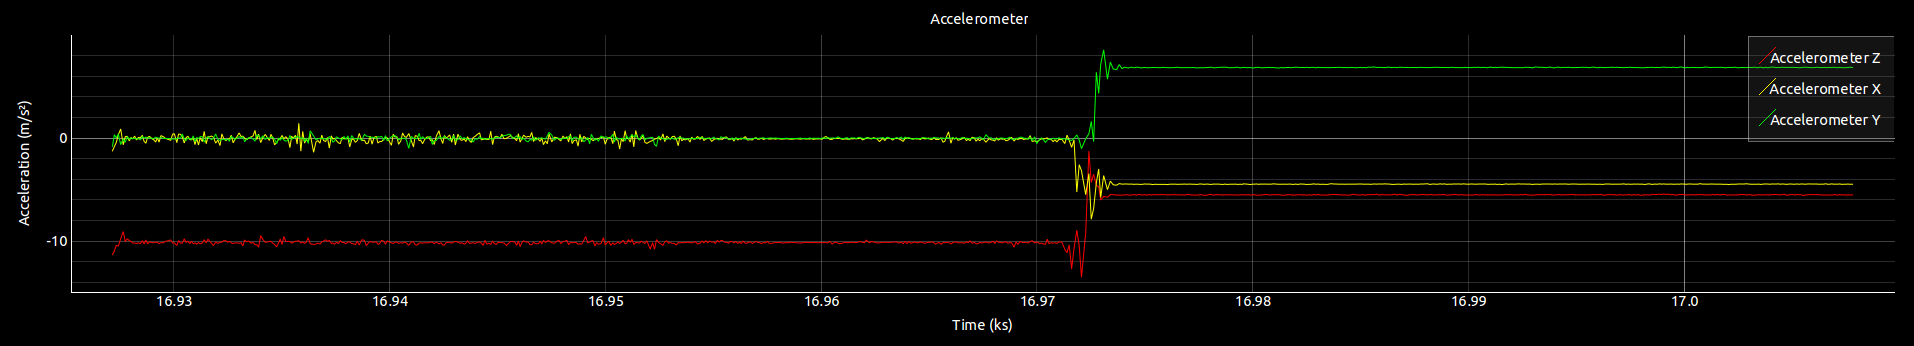
\includegraphics[width=15cm]{images/analyse_1.png}
	\caption{Analyse d'une anomalie: accéléromètre}
	\label{fig:analyse d'une anomalie: accéléromètre}
\end{figure}

\begin{figure}[h]
	\centering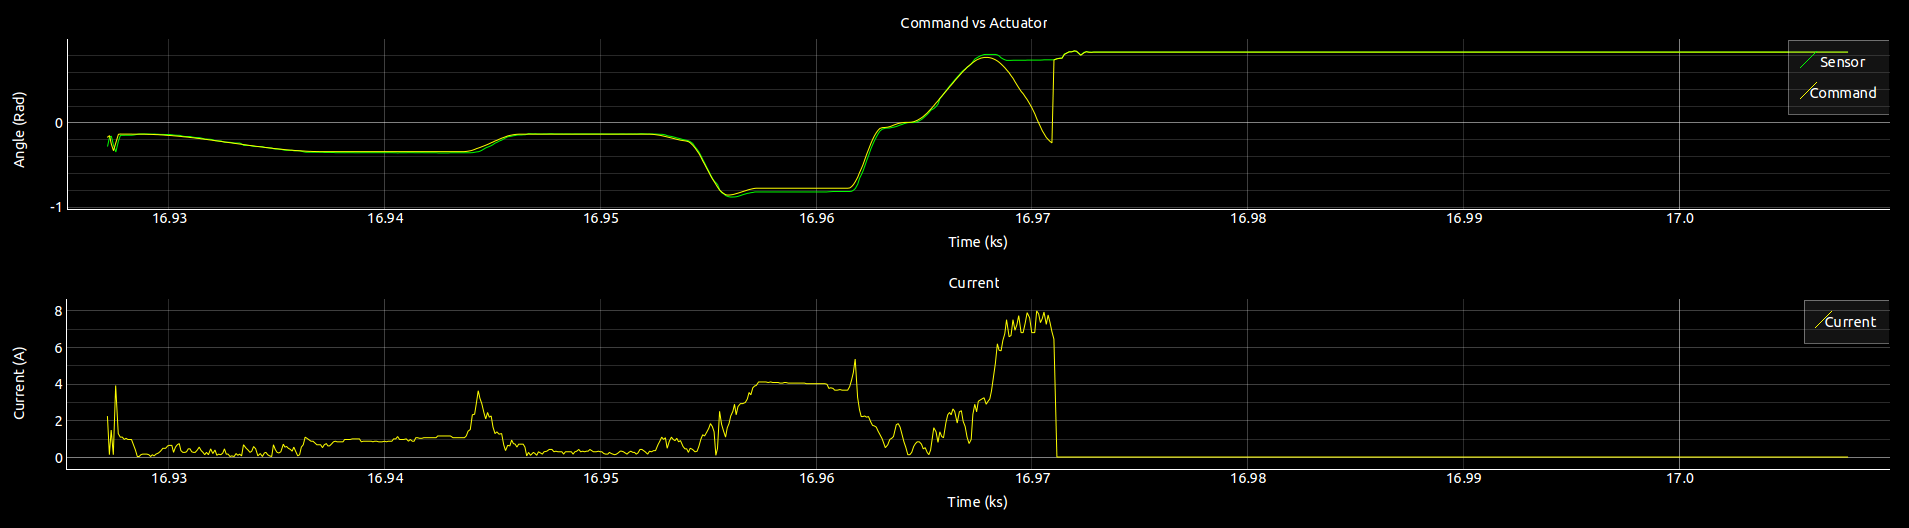
\includegraphics[width=15cm]{images/analyse_2.png}
	\caption{Analyse d'une anomalie: la hanche}
	\label{fig:analyse d'une anomalie: kneePitch}
\end{figure}

\begin{figure}[h]
	\centering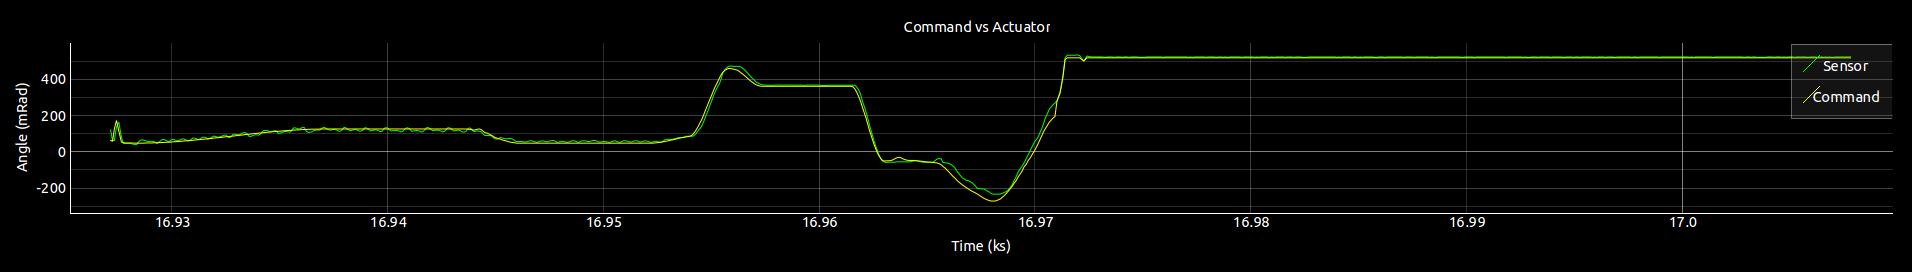
\includegraphics[width=15cm]{images/analyse_3.png}
	\caption{Analyse d'une anomalie: le genou}
	\label{fig:analyse d'une anomalie: hipitch}
\end{figure}

\subsubsection{Hypothèse émise}
 Lors de l'exécution de l'animation "Heat Behavior", le robot est amené à réaliser des mouvements amples au niveau de sa hanche qui causent un certain stress sur cette partie mécanique. Lorsque l'engrenage de la hanche arrive près de sa butée mécanique, un bloquage l'empêche d'atteindre sa position zéro. L'articulation de la hanche ne suit plus sa consigne, ce qui a pour effet de déséquilibrer le robot. Trop déséquilibré, Pepper tombe (\emph{error name}). Une étude plus poussée nous apprendra que la\emph{ root cause } du problème correspondait à un frottement du frein de la hanche. 


\section{Solution proposée}
De part la quantité d'informations à analyser, cette tâche d'analyse peut rapidement devenir rébarbative, d'où le souhait d'automatiser ce processus d'investigation. La variabilité des types de données nous empêche de réduire le nombre d'informations à analyser à de simples caractéristiques communes (e.g. moyenne, écart type, etc.). On s'appuiera donc sur des approches algorithmiques plus poussées, en utilisant notamment des méthodes d'apprentissages automatiques (plus connues sous le terme anglais de Machine Learning). La multiplicité des modèles englobés dans cette discipline nous permettra de répondre au mieux à la problématique.
\chapter{ Le  Machine Learning}
\label{Le Machine Learning}
\thispagestyle{fancy}

\section{Généralités sur le Machine Learning}
\label{Le Machine Learning: Généralités sur le Machine Learning}
Le Machine Learning (traduire par apprentissage automatique) est une ramification de l'intelligence artificielle. Cependant, son statut de subdivision n'informe en rien sur l'étendu des notions contenues dans cette matière scientifique. Son champ d'étude est vaste et en perpétuelle évolution. Les solutions offertes par cette discipline permettent d'étudier toute sortes de données et d'automatiser une multitude de systèmes. L'apprentissage automatique rencontre un succès croissant qui est corrélé avec l'essor des nouvelles technologies et l'automatisation de l'analyse de volumes conséquents de données utilisateurs (Big Data). Les applications sont donc multiples. En voici quelques exemples:  

\begin{itemize}
	\item Algorithmes des moteurs de recherches (Google Deep Dream, Google TensorFlow)
	\item Analyse boursière
	\item Analyse de rapports d'erreurs
	\item Reconnaissance vocale, biométrie, reconnaissance d'écriture
	\item Robotique (vision, mouvements, prise de décision, etc.)
	\item Neurosciences 
\end{itemize}

\subsection{Définition et principe général du Machine Learning}
\label{Le Machine Learning: Généralités sur le Machine Learning: Définition et principe général}
Le champ d'étude et d'application du Machine Learning étant immense, on propose de redéfinir cette notion en l'adaptant à la résolution de notre problématique (i.e. automatiser l'analyse d'incidents révélés lors du filtering test).
On offre ici deux définitions de l'apprentissage automatique: une première dite "High Level" qui le caractérise de manière générale et une seconde qui reflète sa dimension algorithmique. 

\begin{description}
	\item[High Level]: Le Machine Learning permet à un système d'évoluer grâce à un processus d'apprentissage et ainsi de remplir des tâches qu'il est difficile, voir impossible, de remplir par d'autres moyens algorithmiques plus classiques. 
	\item[Mathématique] Le Machine Learning fourni les outils pour prédire une/des donnée(s) de sortie Y à partir des données d'entrée X via un processus d'apprentissage. 
\end{description}
 
 De nombreuses autres définitions existent, mais elles ne correspondent pas à la dimension recherchée dans le cadre de ce projet.
 
Au regard des deux définitions stipulées ci-dessus, on peut définir le principe de base de l'apprentissage automatique sous la forme d'un schéma bloc 	ref{fig:Schéma fonctionnel haut niveau du Machine Learning}.

\begin{figure}[h]
	\centering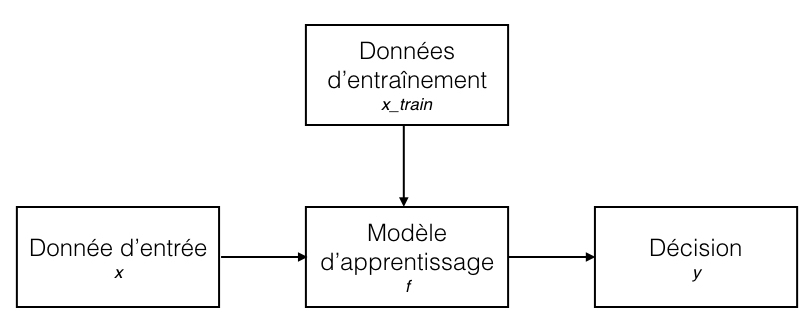
\includegraphics[height=5cm]{images/ML_high_level.jpeg}
	\caption{Schéma fonctionnel haut niveau du Machine Learning}
	\label{fig:Schéma fonctionnel haut niveau du Machine Learning}
\end{figure}

L'apprentissage automatique peut donc être vu dans sa globalité comme un processus composé de deux étapes successives : 
\begin{enumerate}
		\item [Apprentissage]
		 \begin{enumerate}
			\item  Un ensemble de données est présenté au système (X\_train).
			\item A partir de ces informations, le système (f) apprend - s'entraîne- afin d'être par la suite en capacité de prendre décision vis à vis de la tâche qui lui sera demandée. 
		\end{enumerate}
		
		\item [Prise de décision] 
		\begin{enumerate}
			\item  On a en entrée du système une ou des donnée(s) brutes (X).  
			\item Cette donnée est traitée et analysée par le système.
			\item En sortie, une décision est prise quant à la tâche demandée (Y). 
		\end{enumerate}
\end{enumerate}

\subsubsection{Un exemple concret}
\label{Le Machine Learning: Généralités sur le Machine Learning: Définition et principe général:un exemple concret}
Afin de présenter de manière plus concrète le processus fonctionnel haut niveau d'un algorithme d'apprentissage, on présente l'exemple suivant:

\textit{On cherche à déterminer à quelle période de l'année nous nous trouvons (i.e. printemps, été, automne ou hiver) à partir de l'humidité, la température et la pression atmosphérique d'aujourd'hui. \\
	La première étape de notre processus sera donc d'entrainer notre système afin que celui-ci soit en mesure de prendre une décision vis à vis des données qu'on lui présentera en entrée (i.e. l'humidité, la température et la pression atmosphérique d'aujourd'hui). \\
	Une fois le système entrainé, on attend que celui-ci ai ce type de comportement : \\
	On présente en entrée de mon système une température de -2 degrés, une pression atmosphérique de 1030hPa et un taux d'humidité de 81\%. La réponse attendue en sortie du système est: hiver}

On peut adapter le schéma fonctionnel haut niveau du Machine Learning à notre exemple \ref{fig:Schéma fonctionnel haut niveau du Machine Learning, l'exemple prévision saisonnière}. 

\begin{figure}[h]
	\centering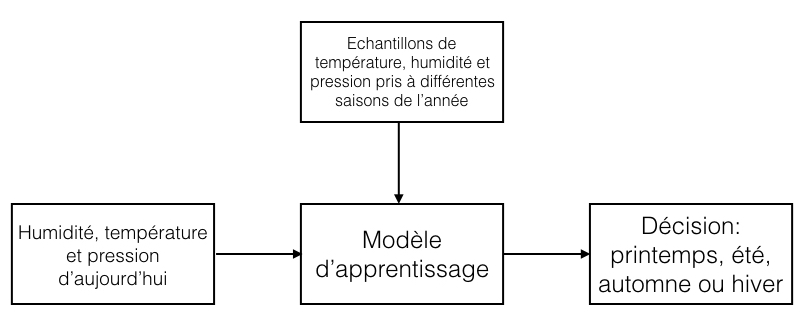
\includegraphics[height=5cm]{images/ML_high_level_expl.jpeg}
	\caption{Schéma fonctionnel haut niveau du Machine Learning, l'exemple de la prévision saisonnière}
	\label{fig:Schéma fonctionnel haut niveau du Machine Learning, l'exemple prévision saisonnière}
\end{figure}

Pour caractériser et  désigner plus précisément les différents éléments de notre système, on présente ci-dessous le champs lexical utilisé dans le domaine du Machine Learning:

\subsubsection{Lexique} 
\begin{description}
	\item [les features] Le type de données présenté en entrée. \\
	\textit{La température, la pression atmosphérique et l'humidité.}
	\item [échantillons ou exemples] Les données permettant d'entrainer le système (x\_train). \\
	\textit{De nombreux échantillons de température, pression atmosphériques et humidité pris à différents périodes de l'année, sur plusieurs années.}
	\item [le modèle d'apprentissage] Le cœur du système décisionnel (f).
	\item [La décision] La sortie ou réponse du système (Y) \\
	\textit{Printemps, été, automne ou hiver.}
\end{description}

\subsection{Les exemples}
\label{Le Machine Learning: Généralités sur le Machine Learning: Les données}
Les exemples correspondent aux données utilisées pour entraîner mon algorithme d'apprentissage. On parle également d'échantillons. Celles-ci sont regroupées en "features" (terme anglais, traduire par caractéristiques). 
Pour reprendre l'exemple cité précédemment \ref{Le Machine Learning: Généralités sur le Machine Learning: Définition et principe général:un exemple concret}, nos données sont regroupées en 3 features: la température, l'humidité et la pression atmosphérique. On données sont donc structurées de la manière suivante: 

\begin{equation}
\begin{blockarray}{cccc}
& température (\degres C) & humidite (\%) & pression(HPa) \\
\begin{block}{c(ccc)}
Exemple_1 & -10 & 85 & 1023 \\
Exemple_2 & 15 & 80 & 1020 \\
Exemple_3 & 23 & 65 & 1015 \\
... & ... & ... & ... \\
Exemple_n & 10 & 81 &  1032 \\
\end{block}
\end{blockarray}
\end{equation}

\subsubsection{Différents types de données}
Il existe deux types de données: les données labellisées et non labellisées.
\begin{itemize}
	\item Les données labellisées correspondent à des exemples corrélés à une sortie - un label - connue.
	\item Les données non labellisées ne sont quant à elles pas associées à une sortie. 
\end{itemize}

Pour reprendre l'exemple précédent \ref{Le Machine Learning: Généralités sur le Machine Learning: Définition et principe général:un exemple concret}, on a les jeux de données suivants: 

\textbf{Données labellisées} 
\begin{equation}
\begin{blockarray}{ccccc}
& température (\degres C) & humidite (\%) & pression(HPa) \\
\begin{block}{c(ccc)c}
Exemple_1 & -10 & 85 & 1023 & hiver\\
Exemple_2 & 15 & 80 & 1020 & automne\\
Exemple_3 & 23 & 65 & 1015 & ete \\
... & ... & ... & ... \\
Exemple_n & 10 & 81 &  1032 & printemps\\
\end{block}
\end{blockarray}
\end{equation}
On connait la sortie qui correspond aux données d'entrée, i.e. que on sait à quelle période de l'année les échantillons ont été prélevé.
 
\textbf{Données non labellisées} 
\begin{equation}
\begin{blockarray}{ccccc}
& température (\degres C) & humidite (\%) & pression(HPa) \\
\begin{block}{c(ccc)c}
Exemple_1 & -10 & 85 & 1023 & ??\\
Exemple_2 & 15 & 80 & 1020 & ??\\
Exemple_3 & 23 & 65 & 1015 & ?? \\
... & ... & ... & ... \\
Exemple_n & 10 & 81 &  1032 & ??\\
\end{block}
\end{blockarray}
\end{equation}
On ne connait pas la sortie qui correspond aux données d'entrée, i.e. que on \emph{ne} sait \emph{pas} à quelle période de l'année les échantillons ont été prélevé. 

\subsection{La décision}
\label{Le Machine Learning: Généralités sur le Machine Learning: La décision}
La sortie de notre système peut être également nommé décision. Toujours selon notre exemple \ref{Le Machine Learning: Généralités sur le Machine Learning: Définition et principe général:un exemple concret}, cela correspond au choix fait par l'algorithme entre les différentes saisons: printemps, été, automne et hiver.  

\subsubsection{Différents types de sorties}
Il existe différents types de sortie: les sorties continues et discrètes.

\begin{description}
	\item [Les sorties continues] peuvent prendre n'importe quelle valeur. \\
	 $y \in R$ \\
	 Déterminer l'évolution de la température en fonction des échantillons enregistrés les mois précédents correspond à une sortie continue.
	\item [Les sorties discrètes] ne peuvent prendre que des valeurs prédéterminées. \\
	 $y \in {1, 2, 3, ...,C}$ \\
	 L'exemple \ref{Le Machine Learning: Généralités sur le Machine Learning: Définition et principe général:un exemple concret} a une sortie discrète. En effet, la sortie ne peut prendre que des valeurs prédéterminées: printemps, été, automne et hiver.
\end{description}


\subsection{Le modèle}
\label{Le Machine Learning: Généralités sur le Machine Learning: Le modèle}
Il existe différents types d'apprentissages. Le choix d'un modèle en particulier est influencé par le type d'exemples que l'on a en entrée du système et du type de décision que l'on souhaite obtenir en sortie. Nous nous intéresserons à différentes catégories d'apprentissages automatiques: 
\begin{itemize}
	\item Les apprentissages supervisés et non-supervisés. Cette caractéristique dépend du type d'exemples que l'on a en entrée du système.
	\item Les régression ou les classifications. Cette caractéristique dépend du type de sortie que l'on souhaite obtenir . 
\end{itemize}

\subsubsection{apprentissage supervisé et non supervisé} 
\label{Le Machine Learning: Généralités sur le Machine Learning: Le modèle: apprentissage supervisé et non supervisé}
L'apprentissage supervisé nécessite d'avoir des données labellisées en entrée, i.e. que l'on connait le type de décision que l'on aura en sortie du système en fonction des exemples en entrée: il y'a une corrélation entre la sortie et l'entrée. C'est cette notion qui s'exprime au travers du terme \emph{supervisé}. 
L'apprentissage non supervisé s'appuie quant à lui sur l'utilisation d'une base de donnée non labellisée pour son apprentissage, i.e qu'on ne connait pas le type de décision associé aux exemples en entrée. Dans le cas d'un apprentissage non supervisé, pour parvenir à prendre une décision, l'algorithme devra diviser ce groupes de données hétérogènes en sous-groupes homogènes d'informations similaires. On appelle ces subdivisions des \emph{clusters}.
Afin de matérialiser les différences entres les deux méthodes et les applications possibles pour chacune d'elles, on propose deux exemples \ref {tab: Comparaison des différentes méthodes d'apprentissage}.

\begin{table}[h]
	\begin{tabular}{ | p {2.5cm} | p {6cm} | p {6cm} |}
	\hline
	 & apprentissage supervisé & apprentissage non supervisé \\
	\hline
	\begin{tabular}{c} exemple n\degres1:\\apprendre aux \\ humains \end{tabular}  &
	 Une institutrice souhaite apprendre à ses élèves à différencier un chat d'un chien: c'est la décision qu'on attend d'eux. Pour ce faire, l'éducatrice leur montre différentes photographies de chiens et de chats: ce sont les exemples utilisés pour l'apprentissage. Ces exemples peuvent être segmentés en différentes caractéristiques, comme la taille de l'animal, sa couleur, la longueur du poil, etc: il s'agit des features. Lorsque que l'institutrice leur présente les différentes images, elle stipule clairement si il s'agit d'un chien ou d'un chat: il y'a donc une corrélation entre l'entrée et la sortie de l'apprentissage, il s'agit d'un apprentissage supervisé (figure \ref{fig:Comparaison d'un apprentissage supervisé et non supervisé dans le cadre de l'exemple "apprendre aux humains"},a).&
	 On retrouve cette même institutrice donnant à ses élèves le même exercice à la différence que, contrairement à précédemment, lorsque qu'elle présente les différentes images, elle \emph{ne} stipule \emph{pas} la race de l'animal: il n'y a donc aucune corrélation entre l'entrée et la sortie de l'apprentissage, il s'agit donc d'un apprentissage non supervisé. Pour réussir cet exercice, les enfants devront donc regrouper les animaux en s'appuyant sur leurs similitudes physiques, i.e. leurs features (e.g. taille de l'animal, sa couleur, longueur du poil, etc.). Les élèves ne connaitrons certes pas le nom des deux animaux, mais ils auront su les différencier. C'est la même approche qui est réalisé en apprentissage automatique non supervisé (figure \ref{fig:Comparaison d'un apprentissage supervisé et non supervisé dans le cadre de l'exemple "apprendre aux humains"}, b). \\
	\hline 
	\begin{tabular}{c} exemple n\degres2:\\la météo \ref*{Le Machine Learning: Généralités sur le Machine Learning: Définition et principe général:un exemple concret}\end{tabular} &
	 On reprend l'exemple dans lequel on souhaite prendre une décision quant à la période de l'année à laquelle on se trouve actuellement, en fonction des features humidité, température et pression atmosphérique. Pour se faire, on prélève des échantillons à différentes périodes de l'année en notant à quelle saison ces données ont été prélevées: se sont des exemples labellisées, i.e. il y'a une corrélation entre les données et la sortie du système. Il s'agit donc d'un apprentissage supervisé (figure \ref{fig:Comparaison d'un apprentissage supervisé et non supervisé dans le cadre de l'exemple prévision saisonnières}, a). &
	On reprend le même problème mais cette fois-ci on ne note pas la saison à laquelle les échantillons ont été prélevé. Pour résoudre le problème, l'algorithme doit donc associer les données les plus similaires entre elles et ainsi créer des groupes homogènes d'informations qui correspondront aux 4 décisions possibles (figure \ref{fig:Comparaison d'un apprentissage supervisé et non supervisé dans le cadre de l'exemple prévision saisonnières}, b). \\
	\hline
	\end{tabular}
	\caption[Comparaison des différents modèles d'apprentissage]{Comparaison de l'apprentissage supervisé et non supervisé par des exemples}
	\label {tab: Comparaison des différentes méthodes d'apprentissage}
\end{table}

%inverser les labels taille et longueur du pelage
\begin{figure}[h]
	\centering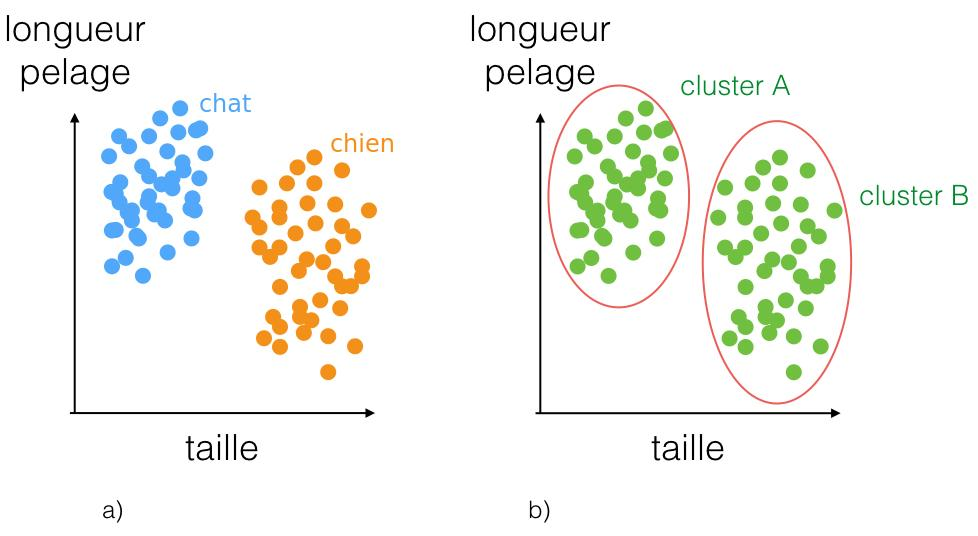
\includegraphics[height=7cm]{images/apprentissage_chat.jpeg}
	\caption[Comparaison d'un apprentissage supervisé et non supervisé dans le cadre de l'exemple "apprendre aux humains"]{Comparaison d'un apprentissage supervisé et non supervisé dans le cadre de l'exemple "apprendre aux humains". On observe sur la figure a) les différents exemples d'entrainement exprimés dans un repère composé des deux features "taille" et "longueur de pelage". On remarque qu'il y'a la formation de deux groupes de données homogènes: les animaux de taille globalement élevée avec un pelage court et les animaux de taille moindre avec un poil globalement plus long. Les données étant labellisées, on sait que le premier groupe correspond à des chiens et le deuxième à des chats.}
	\label{fig:Comparaison d'un apprentissage supervisé et non supervisé dans le cadre de l'exemple "apprendre aux humains"}
\end{figure}

\begin{figure}[h]
	\centering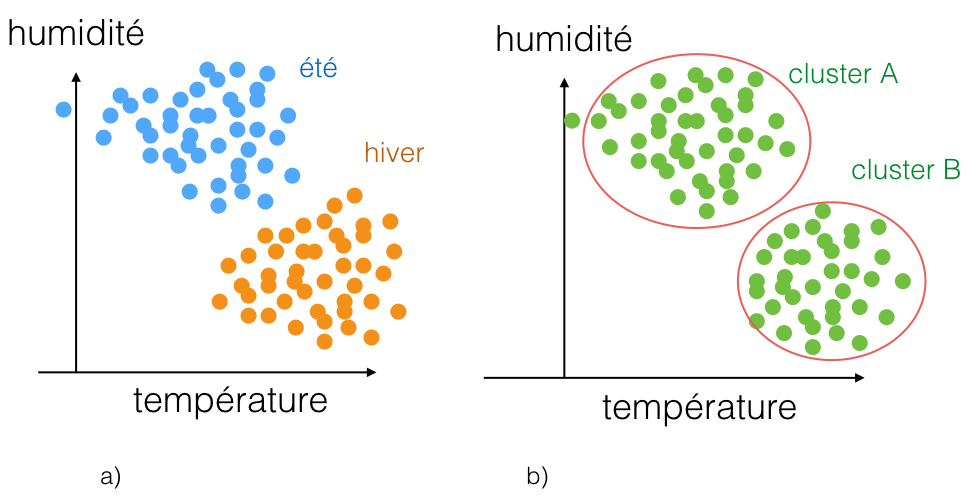
\includegraphics[height=7cm]{images/apprentissage_meteo.jpeg}
	\caption[Comparaison d'un apprentissage supervisé et non supervisé dans le cadre de l'exemple "prévisions saisonnières"]{Comparaison d'un apprentissage supervisé et non supervisé dans le cadre de l'exemple "prévisions saisonnières". On observe sur la figure a) les différents exemples d'entrainement exprimés dans un repère composé des deux dimensions (features) "humidité" et "température". On remarque qu'il y'a la formation de deux groupes de données homogènes: un où les échantillons sont pris lors de saisons globalement chaudes et sèches etc un autre où les échantillons sont enregistrés lors de périodes globalement froides et humides. Les données étant labellisées, on sait que le premier groupe correspond à l'été et l'autre groupe l'hiver.}
	\label{fig:Comparaison d'un apprentissage supervisé et non supervisé dans le cadre de l'exemple prévision saisonnières}
\end{figure}

Il existe deux types d'apprentissage supervisé: la régression et la classification.

\subsubsection{Apprentissage supervisé: régression et classification} 
\label{Le Machine Learning: Généralités sur le Machine Learning: Le modèle:Regression et classification}
 La régression est un type d'apprentissage avec lequel on souhaite obtenir une sortie continue. Dit de manière différente, la régression implique que l'on souhaite \emph{estimer} ou \emph{prédire} une réponse. La classification est quant à elle un type d'apprentissage avec lequel on souhaite obtenir une sortie discrète, elle peut être vu comme un cas particulier de la régression où les valeurs à prédire sont discrètes. Formulé autrement, la classification implique que l'on souhaite \emph{classer} un exemple parmi différentes catégories. Afin de représenter concrètement les nuances entre les deux méthodes et les applications possibles pour chacune d'elle, on propose l'exemple tableau \ref {tab: Comparaison des différentes catégories d'apprentissage supervisé}).

\begin{table}[h]
	\begin{tabular}{ | p {7cm} | p {7cm} |}
		\hline
		régression & classification \\
		\hline
		On souhaite connaitre le temps (température et humidité) qu'il fera pendant les jours suivants. Pour cela, on s'appuie sur les différents échantillons de température et d'humidité enregistrés lors des mois et des années précédentes (exemples labellisés). Le fait de déterminer la température des jours suivants relève de la prédiction (figure \ref {tab: Comparaison des différentes catégories d'apprentissage supervisé}, a).  
		 &  L'exemple de la prédiction saisonnière \ref{Le Machine Learning: Généralités sur le Machine Learning: Définition et principe général:un exemple concret} est un problème de classification: on cherche à classer notre donnée d'entrée parmi plusieurs groupes de données homogènes: printemps, été automne ou hiver (figure \ref {tab: Comparaison des différentes catégories d'apprentissage supervisé}, b). \\
		\hline 
	\end{tabular}
	\caption[Comparaison des différentes catégories d'apprentissage supervisé]{Comparaison entre l'apprentissage supervisé de type régression et supervisé de type classification}
	\label {tab: Comparaison des différentes catégories d'apprentissage supervisé}
\end{table}

\begin{figure}[h]
	\centering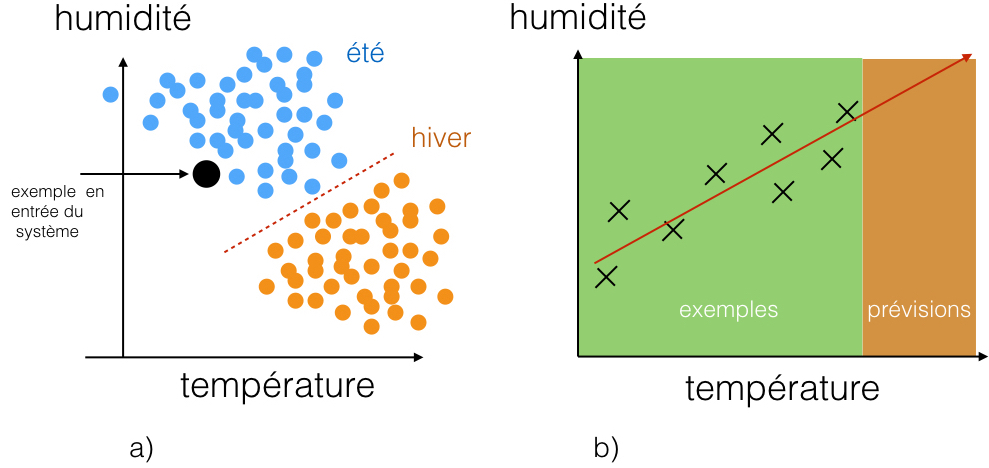
\includegraphics[height=7.5cm]{images/regression_class.jpeg}
	\caption[Comparaison par l'exemple de la régression et la classification]{Comparaison par l'exemple de la régression et la classification. Sur la figure a), on observe deux jeux de données homogènes (été et hiver) s'exprimant dans un repères en deux dimensions (features humidité et température). Le but est ici de classer la donnée en entrée du système parmi ces deux ensembles, il s'agit donc d'un problème de classification. Dans la figure b), on observe une succession d'exemples exprimés dans un repère en deux dimensions (features température et humidité). On remarque une évolution globalement linéaire de ces exemples, nous permettant ainsi de prédire la température et l'humidité sur les prochains mois: il s'agit d'un problème de régression.}
	\label{fig:Comparaison par l'exemple de la régression et la classification}
\end{figure}

\section{Les différents algorithmes d'apprentissage supervisé}
\label{Le Machine Learning:Les différents algorithmes d'apprentissage supervisé}
Il existe différents algorithmes d'apprentissage supervisé utilisés pour résoudre des problèmes de régression et de classification. 

\subsection{La régression linéaire}
\label{Le Machine Learning:Les différents algorithmes d'apprentissage supervisé: La regression linéaire}
La régression linéaire cherche à expliquer une variable de sortie $Y$ par une fonction affine de $X$. Cette fonction linéaire affine est appelée \emph{hypothèse} (notée $h(x)$). Exprimé autrement, on a un jeu de données $X$ auquel correspond un jeu de données $Y$, on cherche les valeurs $\theta_1$ et $\theta_2$ permettant de "mapper" les données, tel que:

\begin{equation}
	h_\theta (x) = \theta_0 + \theta_1 x
\end{equation}

\subsubsection{Exemple de régression linéaire uni-variable}
\label{Le Machine Learning:Les différents algorithmes d'apprentissage supervisé: La regression linéaire: Exemple de régression linéaire uni-variable}
On souhaite déterminer le prix d'un logement en fonction de sa surface au sol en se basant sur les exemples de prix connus du parc immobilier. 
La surface au sol est donc l'entrée $X$ de notre système et le prix la sortie $Y$. Soit le tableau \ref {tab:parc immobilier} les exemples $X$, on obtient la représentation graphique en figure 	\ref{fig:évolution du prix de l'immobilier en fonction de la surface}. Grâce à l'expression de l'hypothèse, on est capable de déterminer le prix d'un loyer en fonction de la surface au sol.  

\begin{table}[h]
	\begin{tabular}{ | p {4cm} | p {4cm} |}
		\hline
		taille ($m^2$) & prix (\euro) \\
		\hline
		2104 & 460 \\
		1416 & 232 \\
		1534 & 314 \\
		852 & 178 \\
		500 & 100 \\ 
		1012 & 212 \\
		126 & 75 \\
		1775 & 432 \\
		600 & 150 \\
		2114 & 510 \\
		1316 & 270 \\
		1634 & 334 \\
		\hline 
	\end{tabular}
	\caption[parc immobilier]{exemples du prix des logements en fonction de leur taille}
	\label {tab:parc immobilier}
\end{table}

\begin{figure}[h]
	\centering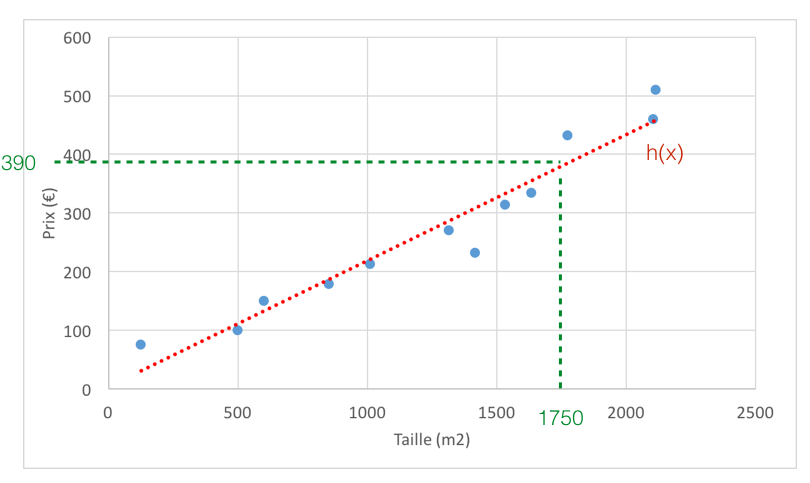
\includegraphics[height=8cm]{images/graph_immobilier.png}
	\caption[évolution du prix de l'immobilier en fonction de la surface]{évolution du prix de l'immobilier en fonction de la surface. L'ensemble des données semble globalement évoluer de manière linéaire. Cette linéarité est représentée par l'hypothèse $h(x)$. Grâce à celle-ci, on peut déterminer le prix d'un logement en fonction de sa superficie, et inversement. Par exemple, un appartement d'une surface de 1750 $m^2$ coutera aux alentours de 390\euro.}
	\label{fig:évolution du prix de l'immobilier en fonction de la surface}
\end{figure}

Cet exemple est dit uni-variable car un seul jeu de données $X$ (superficie) correspond à un jeu de données $Y$ (prix).

\subsubsection{Déterminer les paramètres de l'hypothèse}
\label{Le Machine Learning:Les différents algorithmes d'apprentissage supervisé: La regression linéaire: Déterminer les paramètres de l'hypothèse}

\paragraph{La fonction cout} La fonction coût (en anglais cost function) correspond à la comparaison de la moyenne des différences entre les résultats de l'hypothèse $h(x)$ avec les entrées $X$ et les sorties actuelles $Y$. Cela signifie qu'elle cherche à minimiser les valeurs calculées via l'hypothèse et les valeurs réelles (figure \ref{fig:Régression linéaire, optimisation de la fonction coût}). Soit: 
\begin{equation}
	J(\theta_0,\theta_1) = \frac{1}{2m}\sum_{i=1}^{m}(h_\theta(x^i)-y^{i})^2
\end{equation}

avec:
\begin{itemize}
	\item $J$ la fonction coût
	\item $\theta_0$ et $\theta_1$ les paramètres de l'hypothèse $h(x)$
	\item $m$ le nombre d'exemples disponibles pour l'entrainement 
	\item $h_\theta(x)$ l'hypothèse $h_\theta (x) = \theta_0 + \theta_1 x$
	\item $X^i$ l'exemple
	\item $Y^i$ la sortie 
\end{itemize}


\begin{figure}[h]
	\centering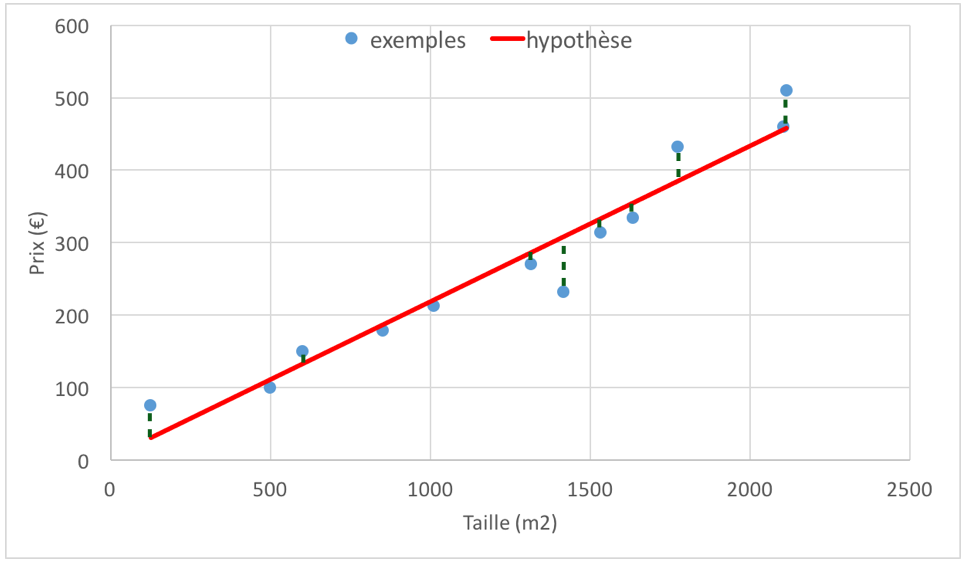
\includegraphics[height=7cm]{images/cost.png}
	\caption[Régression linéaire, optimisation de la fonction coût]{Régression linéaire, optimisation de la fonction coût. les valeurs calculées via l'hypothèse et les valeurs réelles. Cela revient à minimiser la distance entre un exemple et l'hypothèse.}
	\label{fig:Régression linéaire, optimisation de la fonction coût}
\end{figure}

On cherchera donc à minimiser la valeur de a fonction coût $J(\theta_0,\theta_1)$. En jouant sur la valeur des paramètres $\theta_0$ et $\theta_1$ de l'hypothèse. Pour cela, on calcule la fonction coût pour différentes valeurs de $\theta_0$ et $\theta_1$ et on cherche la valeur minimale de $J(\theta_0,\theta_1)$ (figure \ref{Régression linéaire, calcul des paramètres de l'hypothèse}). Dans l'idée, cela revient à choisir une valeur de $\theta$ et de "faire un pas" vers la direction la plus basse, il s'agit donc d'un calcul itératif. Mathématiquement, trouver le minimum peut être déterminé en appliquant l'algorithme du gradient (en anglais, gradient descent), tel que:

\begin{equation}
	\begin{split}
		\theta_0 = \theta_0 - \alpha \frac{\partial J(\theta_0,\theta_1)}{\partial\theta_0} \\
		\theta_1 = \theta_1 - \alpha \frac{\partial J(\theta_0,\theta_1)}{\partial\theta_1}
	\end{split}
\end{equation}

avec $\alpha$ la taille du "pas" que l'on fait vers la direction la plus basse. Si la valeur de $\alpha$ est trop petite, le nombre d'itération sera plus important, augmentant ainsi le temps de calcul. Si la valeur de $\alpha$ est trop grande, on risque de ne pas atteindre le minimum et de diverger.  

\begin{figure}[h]
	\centering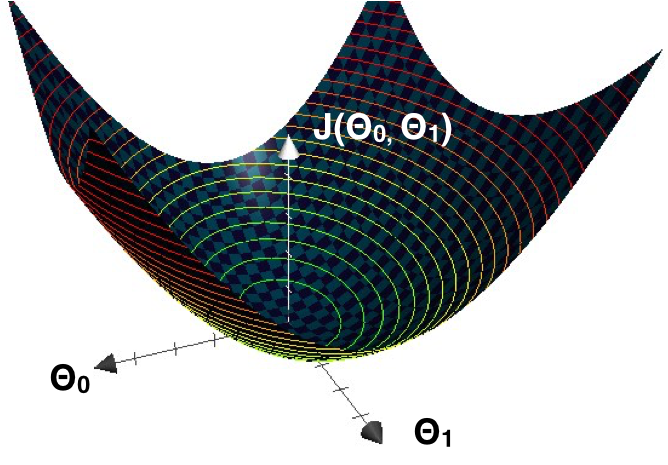
\includegraphics[height=7cm]{images/gradient.jpeg}
	\caption[Régression linéaire, calcul des paramètres de l'hypothèse]{Régression linéaire, calcul des paramètres de l'hypothèse. Ce graphique représente la variation des paramètres $\theta_0$ et $\theta_1$ de l'hypothèse en fonction de la valeur de la fonction coût. On cherche les valeurs  $\theta_0$ et $\theta_1$ minimisant$J(\theta_0,\theta_1)$. La courbe ayant la forme d'une cuvette, les valeurs optimales de $\theta_0$ et $\theta_1$ correspondent à celles au fond de la cuvette.}
	\label{fig:Régression linéaire, calcul des paramètres de l'hypothèse}
\end{figure}
 
\subsection{La régression logistique}
\label{ILe Machine Learning: Les différents algorithmes: La regression logistique}

\subsection{Les réseaux neuronaux}
\label{ILe Machine Learning: Les différents algorithmes: Les réseaux neuronaux}

\subsection{SVM - Support Vector Machine-}
\label{ILe Machine Learning: Les différents algorithmes: SVM}

\subsection{Comparaison des algorithmes}
\label{ILe Machine Learning: Les différents algorithmes: Comparaison des algorithmes}
\chapter{Automatisation du processus d'investigation}
\label{Automatisation du processus d'investigation}
\thispagestyle{fancy}
Lorsqu'une \emph{error name} est révélée durant le Filtering test, de nombreuses données sont enregistrées dans un fichier journal (que l'on retrouve plus souvent sous le terme anglais de fichier "log".) Une analyse poussée de ces informations permet de déterminer la \emph{root cause} liée à l'\emph{error name} (partie \ref{Introduction:Expression du besoin:Hiérarchisation des erreurs}). Afin d'automatiser ce processus d'analyse, on s'appuie sur l'utilisation d'algorithmes d'apprentissage automatique. 

\section{Architecture High Level du système proposé}
\label{Automatisation du processus d'investigation: Achitecture High Level du système proposé}
L'architecture haut niveau de la solution que l'on propose est composée de deux couches: une couche \emph{root cause} et une couche \emph{error name}.
\begin{description}
	\item [Couche root cause] La couche \emph{root cause} permet de détecter la présence d'une \emph{root cause} dans le fichier log que l'on analyse. Il s'agit d'un algorithme d'apprentissage automatique entraîné à effectuer cette tâche.
	\item [Couche error name] La couche \emph{error name} est constituée d'un ensemble de couches \emph{root cause} de telle manière que lorsqu'un fichier log est mis en entrée du système, l'ensemble des couches \emph{root cause} sont activées. Ainsi, le système recherche la présence de chaque \emph{root cause} connue dans l'exemple étudié. On dit que les \emph{root causes} sont liées à l'\emph{error name}. On obtient en sortie de la couche \emph{error name} le nom de la \emph{root cause} ayant la plus forte probabilité d'avoir été reconnue.
\end{description} 

\subsubsection{Exemple de mise en place  d'une couche error name et de ses couches root cause}
\label{Automatisation du processus d'investigation: Achitecture High Level du système proposé: Exemple de mise en place  d'une couche error name et de ses couches root cause}
Afin d'exposer de manière concrète le fonctionnement de l'architecture haut niveau de la solution proposée, on soumet un exemple de mise en place d'une architecture de détection et son utilisation. \\

\paragraph{Mise en place du système de détection d'une root cause}
On souhaite dans un premier temps mettre en place l'architecture permettant de détecter la cause (\emph{root cause}) ayant entrainé la chute du robot lors du Filtering test (\emph{error name}). Cette étape consiste à créer les couches \emph{root cause}, i.e. entrainer différents algorithmes d'apprentissage automatique à reconnaître la \emph{root cause} pour laquelle ils ont été créés (figure \ref{fig:Creation des couches root cause}). Afin d'entraîner ces couches, on utilise les données utiles à chaque \emph{root cause}, contenues dans le fichier log généré lors de la chute d'un robot durant le Filtering Test. Par exemple, dans le cas de la \emph{root cause} "frottement des freins de la hanche", on utilisera les données "valeurs du senseur de la hanche" et "valeurs de l'actuateur de la hanche". Ces deux éléments correspondent aux features de notre système d'apprentissage (c.f. partie \ref{Le Machine Learning: Généralités sur le Machine Learning: Définition et principe général:Lexique}). L'ensemble de ces couches \emph{root cause} sont liées une couche \emph{error name}, ici la chute d'un robot.

\begin{figure}[h]
	\centering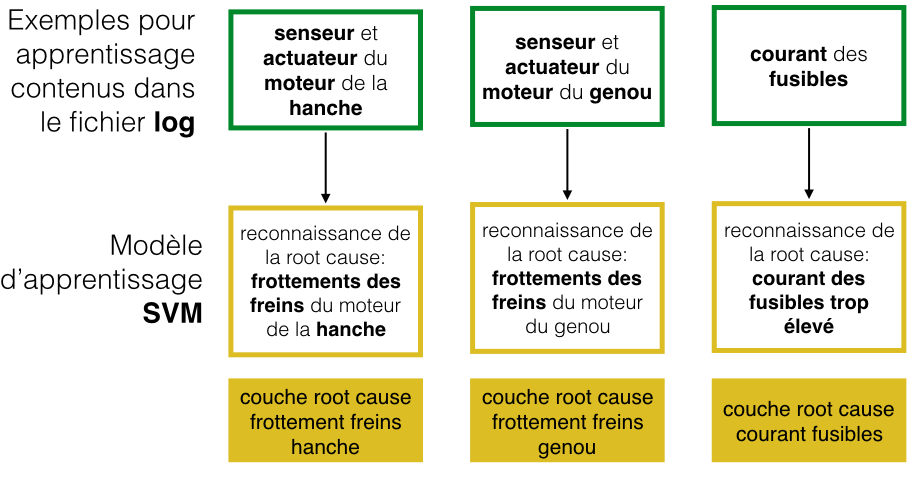
\includegraphics[height=7cm]{images/synoptique_root.png}
	\caption[Création des couches root cause]{Synoptique haut niveau de la création des couches \emph{root cause}. Les couches \emph{root cause} correspondent à des algorithmes d'apprentissage automatique que l'on entraîne à détecter la \emph{root cause} à laquelle ils sont associés. Par exemple, créer la couche \emph{root cause} "frottement du frein de la hanche" revient à entraîner un algorithme d'apprentissage de type SVM, à partir des valeurs senseurs et actuateurs de la hanche des fichiers logs.}
	\label{fig:Creation des couches root cause}
\end{figure}

\paragraph{Utilisation du système de détection d'une root cause}
Une fois nos différentes couches \emph{root cause} créées, on souhaite utiliser notre système pour détecter la cause ayant entrainé la chute d'un robot (cf. figure \ref{fig:utilisation de la couche error name}). Pour cela, on place à l'entrée de notre couche \emph{error name} le fichier log que l'on souhaite analyser. Chaque couche \emph{root cause} extrait de ce fichier les features qui lui sont liées (e.g. la \emph{root cause} "frottement des freins de la hanche" est liée aux features senseurs et actuateurs de la hanche). L'algorithme SVM de chaque couche \emph{root cause} va alors émettre une décision quant à la présence ou non de leur \emph{root cause} dans le fichier log. Cette décision correspond à la probabilité que la \emph{ root cause} ait été détectée (en \%). La couche \emph{root cause} ayant la probabilité la plus élevée en sortie est considérée comme la \emph{root cause} ayant entrainé l'\emph{error name},  ici la chute du robot) 

\begin{figure}[h]
	\centering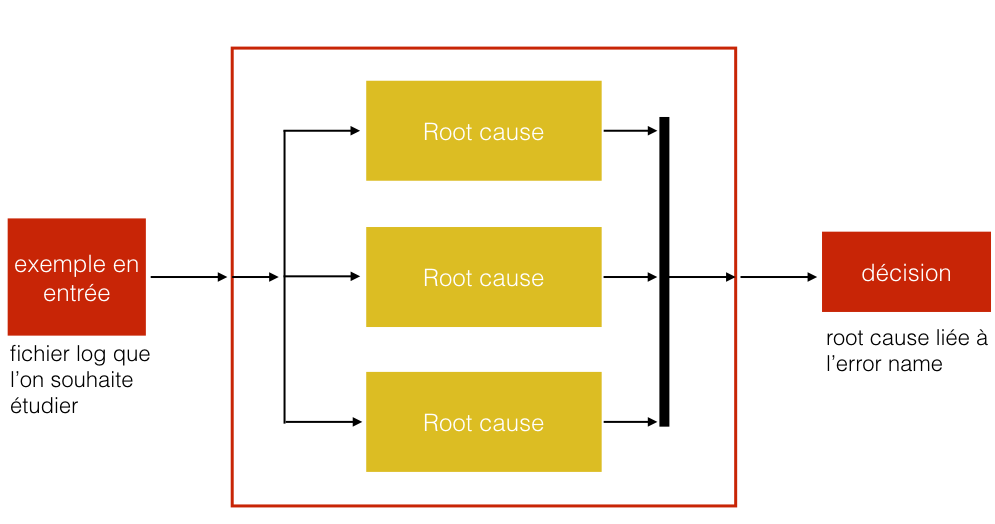
\includegraphics[width=15cm]{images/synoptique_error.png}
	\caption[Utilisation de la couche error name]{Synoptique haut niveau de l'utilisation de la couche \emph{error name}. La couche \emph{error name} contient plusieurs couches \emph{root cause} (on dit qu'elles sont liées). On met en entrée du système le fichier log que l'on souhaite analyser, puis chaque couche \emph{root cause} va détecter la présence de sa \emph{root cause}. On obtient en sortie de la couche \emph{error name} la \emph{root cause}  ayant eu la plus forte probabilité d'avoir été reconnue.}
	\label{fig:utilisation de la couche error name}
\end{figure}

Chaque couche \emph{root cause} peut être considérée comme un système d'apprentissage à part entière. Le schéma fonctionnel d'une \emph{root cause} (cf. figure 	\ref{fig:Synoptique d'une couche root cause}) reprend la même structure que celui du Machine Learning (cf. figure \ref{fig:Schéma fonctionnel haut niveau du Machine Learning}). En effet, chaque \emph{root cause} est constituée d'une instance de l'algorithme SVM. Dans la suite de notre étude de l'architecture haut niveau, on s'intéressera plus particulièrement  au fonctionnement de la couche \emph{root cause}, celle-ci contenant l'ensemble du traitement et de l'analyse des données.

\begin{figure}[h]
	\centering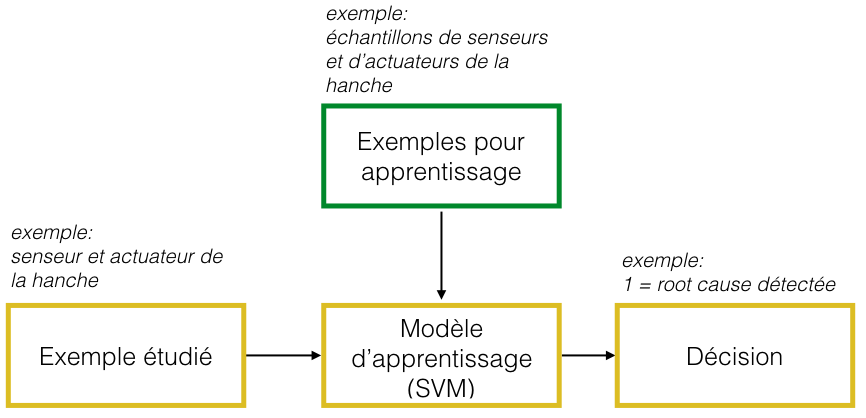
\includegraphics[height=7cm]{images/exemple_root.png}
	\caption[Synoptique d'une couche root cause]{Synoptique d'une couche \emph{root cause}. Il correspond à celui du Machine Learning car chaque couche \emph{root cause} est en réalité un algorithme d'apprentissage supervisé SVM que l'on entraine à détecter une \emph{root cause} particulière.}
	\label{fig:Synoptique d'une couche root cause}
\end{figure}

\subsection{Les exemples}
\label{Automatisation du processus d'investigation: Achitecture High Level du système proposé: Les exemples}
Les exemples sont les éléments permettant d'entraîner un algorithme d'apprentissage automatique (cf. partie \ref{Le Machine Learning: Généralités sur le Machine Learning: Les données}). Dans le cadre de la résolution de notre problématique, ils correspondent aux données générées et enregistrées dans le fichier log lorsqu'une erreur (\emph{error name}) est détectée durant le Filtering Test.

\subsubsection{Structure du fichier log}
\label{Automatisation du processus d'investigation: Achitecture High Level du système proposé: Les exemples: Structure du fichier log}
Le fichier log renferme un ensemble de données enregistrées lors de la détection d'une erreur durant le Filtering Test. Elles correspondent aux "rythmes vitaux" du robot. Le fichier contient par exemple l'évolution temporelle des différents actuateurs et senseurs de Pepper, la température de différentes pièces mécaniques, etc. Dans le cadre de l'entraînement de l'algorithme du Machine Learning (SVM), chacune de ces constantes correspond à une feature  (cf. partie  \ref{Le Machine Learning: Généralités sur le Machine Learning: Définition et principe général:Lexique}). Soit le tableau \ref {tab: Extrait du contenu d'un fichier log}, un extrait du contenu d'un fichier log:

\begin{equation}
\begin{blockarray}{ccccccc}
\begin{block}{c[cccccc]}
features & X_1 & X_2 & X_3 & X_4 &  X_5 & X_6 \\
t_0 & -0,404 & 0,64 & -0,023 & -0,04 & -0,008 & -0,007 \\
t_1 & -0,404 & 0,64 & -0,029 & -0,038 & -0,006 & -0,006 \\
t_3 & -0,404 & 0,576 & -0,029 & -0,033 & -0,008 & -0,012 \\
t_4 & -0,402 & 0,544 & -0,029 & -0,027 & -0,012 & -0,022 \\
t_5 & -0,401 & 0,448 & -0,029 & -0,027 & -0,015 & -0,029 \\
t_6 & -0,401 & 0,448 & -0,023 & -0,029 & -0,017 & -0,031 \\
t_7 & -0,408 & 0,096 & -0,021 & -0,031 & -0,015 & -0,032 \\
t_8 & -0,444 & 0,096 & -0,021 & -0,032 & -0,015 & 0,035 \\
t_9 & -0,486 & 0,096 & -0,021 & -0,033 & -0,017 & -0,039 \\
t_{10} & -0,523 & 0,128 & -0,021 & -0,033 & -0,018 & -0,043 \\
t_n & ... & ... & ... & ... & ... & ... \\
\end{block}
\end{blockarray}
\label {tab: Extrait du contenu d'un fichier log}
\end{equation}

Avec :
\begin{itemize}
	\item $X_1$ = HeadPitchPositionActuatorValue
	\item $X_2$ = HeadPitchElectricCurrentSensorValue
	\item $X_3$ = ipPitchPositionSensorValue
	\item $X_4$ = HipPitchPositionActuatorValue
	\item $X_5$ = KneePitchPositionSensorValue
	\item $ X_6$ = KneePitchPositionActuatorValue
\end{itemize}

Le fichier log, représenté par le tableau \ref {tab: Extrait du contenu d'un fichier log}, correspond à un exemple de la base de données qui sert à entrainer chacun de nos algorithmes. \\ 
A chaque colonne du tableau correspond une feature. Chacune des lignes est la valeur des features à un instant t (une ligne ne correspond pas à un exemple !). 

\subsubsection{Structure de la base de données d'exemples}
\label{Automatisation du processus d'investigation: Achitecture High Level du système proposé: Les exemples: Structure de la base de données d'exemples}
La base de données est composée de plusieurs exemples qui correspondent à des fichiers logs. Par exemple, dans le cadre de la construction de couche \emph{error name} de la chute d'un robot, la base de données sera constituée de fichiers logs générés par plusieurs cas de chutes sur différents robots. On peut représenter la structure des données de la base de données par le tableau \ref {tab: Structure de la base de données d'exemples pour l'entrainement du SVM}

\begin{equation}
\begin{blockarray}{ccccccc}
\begin{block}{c[cccccc]}
features & X_1 & X_2 & X_3 & X_4 &  X_5 & X_6 \\
exemple_0 & log_0 [X_1] & log_0 [X_2] & log_0 [X_3]& log_0 [X_4] & log_0 [X_5] & log_0 [X_6]  \\
exemple_1 & log_1 [X_1] & log_1 [X_2] & log_1 [X_3]& log_1 [X_4] & log_1 [X_5] & log_1 [X_6]  \\
exemple_2 & log_2 [X_1] & log_2 [X_2] & log_2 [X_3]& log_2 [X_4] & log_2 [X_5] & log_2 [X_6]  \\
exemple_3 & log_3 [X_1] & log_3 [X_2] & log_3 [X_3]& log_3 [X_4] & log_3 [X_5] & log_3 [X_6]  \\
exemple_4 & log_4 [X_1] & log_4 [X_2] & log_4 [X_3]& log_4 [X_4] & log_4 [X_5] & log_4 [X_6]  \\
exemple_4 & log_4 [X_1] & log_n [X_2] & log_n [X_3]& log_n [X_4] & log_n [X_5] & log_n [X_6]  \\
\end{block}
\end{blockarray}
\label {tab: Structure de la base de données d'exemples pour l'entrainement du SVM}
\end{equation}

Tout comme la structure d'un fichier log (\ref{Automatisation du processus d'investigation: Achitecture High Level du système proposé: Les exemples: Structure du fichier log}), chaque colonne correspond à une feature. Chaque ligne de ce tableau représente un exemple et correspond à un fichier log. Cela signifie que chaque ligne du tableau correspond au contenu d'un fichier log, présenté dans le tableau \ref {tab: Extrait du contenu d'un fichier log}.

\subsubsection{Construction d'une couche root cause à partir de la base de données d'exemples}
\label{Automatisation du processus d'investigation: Achitecture High Level du système proposé: Les exemples: Construction d'une couche root cause à partir de la base de données d'exemples}
Lorsque l'on veut construire une nouvelle couche \emph{root cause}, i.e. entraîner un nouvel algorithme d'apprentissage, pour détecter la présence d'une \emph{root cause} particulière dans un fichier log, on sélectionne uniquement les features de la base de données d'exemples liées à celle-ci. Par exemple, si on veut créer une nouvelle couche root cause "frottement des freins de la hanche" (lié à l'error name chute du robot), on n'utilisera que les features "HipPitchPositionSensorValue" et "HipPitchPositionActuatorValue" de notre base de données.

\subsubsection{Représentation des exemples et des classes}
\label{Automatisation du processus d'investigation: Achitecture High Level du système proposé: Les exemples: Représentation des exemples et des classes}
Pour construire chaque couche \emph{root cause}, on doit entrainer l'algorithme de l'apprentissage automatique SVM. Pour cela, on a besoin d'exemples labellisés positif (dans notre cas, le terme positif signifie que l'exemple est le motif caractéristique de la \emph{root cause}) et des exemples labellisés négatif (des exemples qui ne correspondent pas au motif caractéristique de la \emph{root cause}). Ces deux groupes de données forment alors des classes. \\
Dans le cadre de la \emph{root cause} "frottement des freins de la hanche", on peut visualiser l'ensemble des exemples et des classes dans un repère construit à partir des features "position du senseur de la hanche" (clé HipPitchPositionSensorValue) et "position de l'actuateur de la hanche" (clé HipPitchPositionActuatorValue) en figure \ref{fig:Représentation de la répartition des exemples et des classes en fonction des features}. Lors de la phase d'investigation, l'algorithme emet alors un choix entre ces deux classes: positive, i.e. présence de la \emph{root cause} dans le fichier log, négative, i.e. absence de la \emph{root cause} dans le fichier log. 

\begin{figure}[h]
	\centering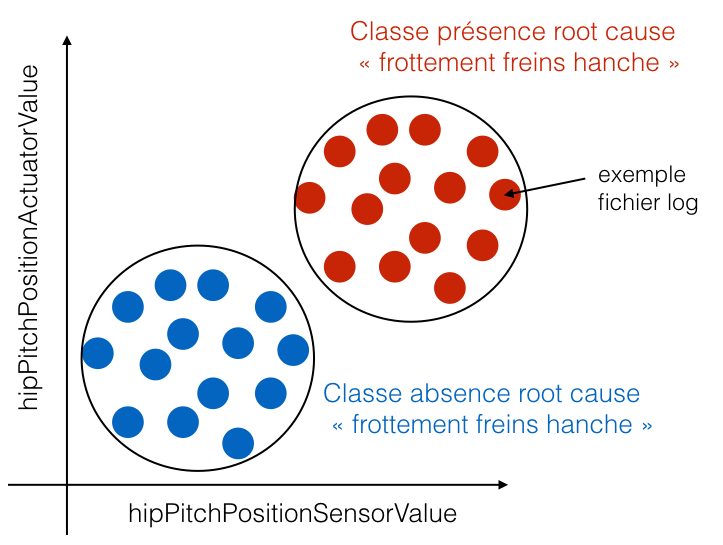
\includegraphics[width=9cm]{images/classes_log.png}
	\caption[Représentation de la répartition des exemples et des classes en fonction des features]{Représentation de la répartition des exemples et des classes en fonction des features. On observe que lorsque l'on visualise les exemples contenus dans nos fichiers logs en fonction des deux features HipPitchPositionSensorValue et HipPitchPositionActuatorValue, ces derniers se regroupent en deux zones homogène qui forment nos classes. Une classe correspond aux exemples de \emph{root cause} "frottement des freins de la hanche", l'autre classe aux exemple qui ne correspondent pas à des exemples de "frottement des freins de la hanche".
	\label{fig:Représentation de la répartition des exemples et des classes en fonction des features}
\end{figure}

Cette représentation n'est pas fonctionnelle mais conceptuelle, i.e. qu'il ne s'agit pas d'une visualisation résultant d'un système fonctionnel mais d'une idée haut niveau que l'on a de la sortie de notre système. 


\subsubsection{Parallèle avec l'exemple de la prévision saisonnière}
\label{Automatisation du processus d'investigation: Achitecture High Level du système proposé: Les exemples: Parallèle avec l'exemple de la prévision saisonnière}
Si on compare les échantillons utilisés dans l'exemple "prévision saisonnière" (cf. tableau \ref{exemples prévision saisonnière}) et ceux de notre solution (c.f. tableau \ref {tab: Structure de la base de données d'exemples pour l'entrainement du SVM}), on observe que dans les deux cas les données sont structurées en exemples et features. Cependant, dans la solution que l'on propose, les données de chaque exemple évoluent temporellement (e.g. la "HipPitchPositionSensorValue" de l'exemple 1 correspond à la colonne "HipPitchPositionSensorValue" du fichier $log_1$, qui a une évolution temporelle), alors que celles de la prévision saisonnière sont discrètes (e.g la température de l'exemple 1 est de -10\degres C, elle est discrète) \\
Or, on ne peut pas réaliser de l'apprentissage supervisé avec des données temporelles. Sous leurs formes actuelles, nos exemples ne peuvent donc pas servir à entrainer les algorithmes SVM de nos couches \emph{root cause}.


\subsection{Le modèle d'apprentissage}
\label{Automatisation du processus d'investigation: Achitecture High Level du système proposé: Le modèle d'apprentissage}
Le modèle d'apprentissage utilisé est le Support Vector Machine (SVM) (cf. partie \ref{Le Machine Learning: Les différents algorithmes: SVM}).


\subsection{La décision}
\label{Automatisation du processus d'investigation: Achitecture High Level du système proposé: La décision}
Chaque couche \emph{root cause} délivre en sortie la probabilité que la \emph{root cause} à laquelle elle est rattachée soit présente dans le fichier log analysé (via le SVM).



\section{Détection d'une root cause}
\label{Automatisation du processus d'investigation: Détection d'une root cause}
On souhaite réaliser de la reconnaissance de motifs grâce à l'utilisation du SVM, pour détecter la présence d'une \emph{root cause} dans un fichier log. L'utilisation de cette méthode répond notamment au problème causé par l'évolution temporelle des exemples utilisés pour l'entraînement de l'algorithme (cf. partie \ref{Automatisation du processus d'investigation: Achitecture High Level du système proposé: Les exemples: Parallèle avec l'exemple de la prévision saisonnière}). On présente dans cette partie les différentes solutions envisagées et les raisons ayant amené à utiliser la reconnaissance de motifs. \\

\subsection{Différentes approches étudiées}
\label{Automatisation du processus d'investigation: Reconnaissance de motifs: Différentes approches étudiées}
L'évolution temporelle des exemples utilisés pour l'entraînement de l'algorithme implique de prétraiter les données (cf. partie \ref{Automatisation du processus d'investigation: Achitecture High Level du système proposé: Les exemples: Parallèle avec l'exemple de la prévision saisonnière}). Pour cela, différentes approches sont envisagées.

\subsubsection{Création de nouvelles features}
\label{Automatisation du processus d'investigation: Reconnaissance de motifs: Différentes approches étudiées: Création de nouvelles features}
On propose de créer de nouvelles features constantes. Elles sont des caractéristiques des features actuelles. Dans le cadre de cette étude, on les identifiera sous l'appellation de \emph{caractéristiques simplifiées}. Elles correspondent par exemple au calcul de la moyenne d'une feature, la valeur crête-à-crête, la valeur maximum, etc. On se sert ensuite de ces  \emph{caractéristiques simplifiées} pour réaliser l'entrainement de l'algorithme d'apprentissage automatique (cf. exemple figure \ref{fig:Calcul de nouvelles features}).

\begin{figure}[h]
	\centering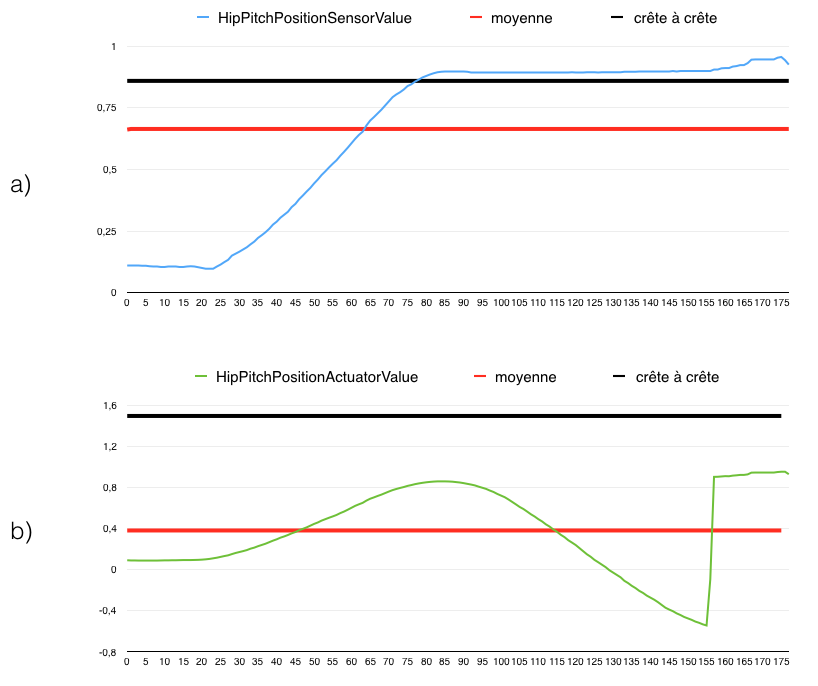
\includegraphics[width=12cm]{images/caracteristiques_simples_1.png}
	\caption[Calcul des caractéristiques simplifiées]{Calcul des \emph{caractéristiques simplifiées}. La figure représente l'évolution de la feature "accélération du robot selon l'axe $z$",  caractéristique de la chute d'un robot. La ligne rouge représente sa valeur moyenne. la ligne noire correspond à sa valeur crête-à-crête. On a ainsi réduit notre feature à deux valeurs constantes. On peut  entraîner l'algorithme d'apprentissage automatique à partir de ces \emph{caractéristiques simplifiées}.}
	\label{fig:Calcul de nouvelles features}
\end{figure}

Le problème de cette approche est qu'elle réduit le nombre d'informations que contient une donnée à seulement quelques features (e.g. moyenne, valeur crête-à-crête). Comme le démontre la figure \ref{fig:Comparaison de deux caractéristiques}, cette diminution des informations peut entrainer des risques de confusion entre différentes features, i.e. deux features différentes peuvent avoir les mêmes caractéristiques. Or, si on souhaite utiliser cette approche dans l'architecture que l'on propose (cf. partie \ref{Automatisation du processus d'investigation: Achitecture High Level du système proposé}), le risque est que deux couches \emph{root cause} soient liées à des features dont les caractéristiques sont similaires. Dans ce cas, le système est incapable de déterminer quelle \emph{root cause} est responsable de l'apparition d'une \emph{error name}.

\begin{figure}[h]
	\centering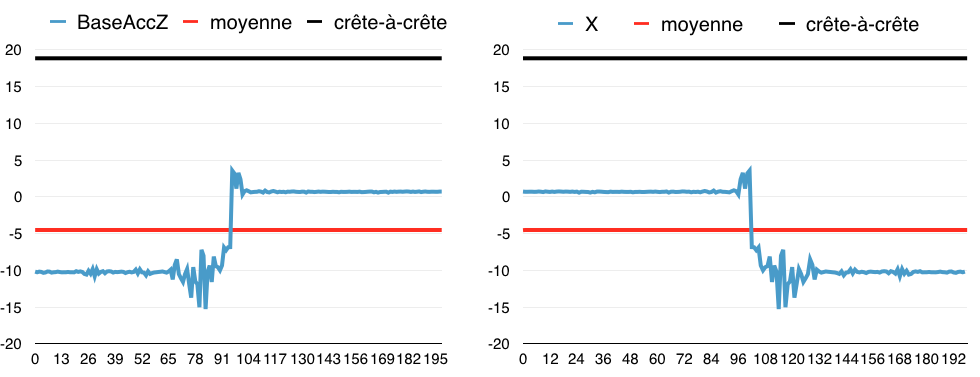
\includegraphics[width=15cm]{images/caracteristiques_simples_2.png}
	\caption[Comparaison de deux caractéristiques]{Comparaison de deux caractéristiques. On retrouve sur la figure a) la valeur de l'accélération selon l'axe $z$ et ses caractéristiques simplifiées. Sur la figure b), on observe une autre feature et ses caractéristiques simplifiées. On remarque que, bien qu'il s'agisse de features différentes entres les figures a) et b), ces dernières possèdent les mêmes \emph{caractéristiques simplifiées}.}
	\label{fig:Comparaison de deux caractéristiques}
\end{figure}

\subsubsection{Considérer chaque unité de temps comme une feature}
\label{Automatisation du processus d'investigation: Reconnaissance de motifs: Différentes approches étudiées: Considérer chaque unité de temps comme une feature}
On propose de considérer chaque unité de temps comme une feature. Le nombre d'entrées du système d'apprentissage automatique est donc égal au nombre d'échantillons contenus dans un exemple. \\
De manière intuitive, entrainer le modèle revient à créer un patron représentatif de la feature lorsque celle-ci est liée à la présence d'une \emph{root cause}. Une fois cette forme apprise, on la compare avec la feature que l'on souhaite analyser afin de savoir si la \emph{root cause} est présente ou non dans la feature.
\newline

\paragraph{Exemple} On souhaite créer une nouvelle couche \emph{root cause} (i.e. entraîner un algorithme d'apprentissage) capable de reconnaitre lorsqu'un robot chute. Dans le cadre de notre problématique ce système n'a pas de réelle utilité, on le propose ici car le problème est simple à comprendre. \\
Pour savoir si le robot chute ou non, on analyse l'évolution de la valeur de l'accélération selon l'axe $z$, fourni par l'accéléromètre de la base de Pepper (clé BaseAccZ). \\
D'après la figure \ref{fig:Formes caractéristiques de BaseAccZ en temps normal et en cas de chute}, on remarque que l'évolution de BaseAccZ, enregistrée lors de la chute d'un robot diffère de l'évolution de BaseAccZ lorsque le robot ne chute pas. On va entraîner à l'algorithme à reconnaitre la forme caractéristique de l'évolution de l'accélération en $z$ lorsque le robot chute. Pour cela, on admet que chaque échantillon (chaque instant t) qui constitue la BaseAccZ devient une entrée (feature) pour l'entrainement de l'algorithme d'apprentissage (cf. figure \ref{fig:Créer un patron caractéristique de la chute du robot}). \\
On compare ensuite ce patron à la courbe de l'accélération en $z$ contenue dans le fichier log que l'on souhaite étudier. Si elle est globalement similaire au patron, on en déduit que le robot a chuté. Dans le cas contraire, on en déduit que le robot n'a pas chuté (cf. figure \ref{fig:Détection d'une chute à partir du patron de BaseAccZ}).

\begin{figure}[h]
	\centering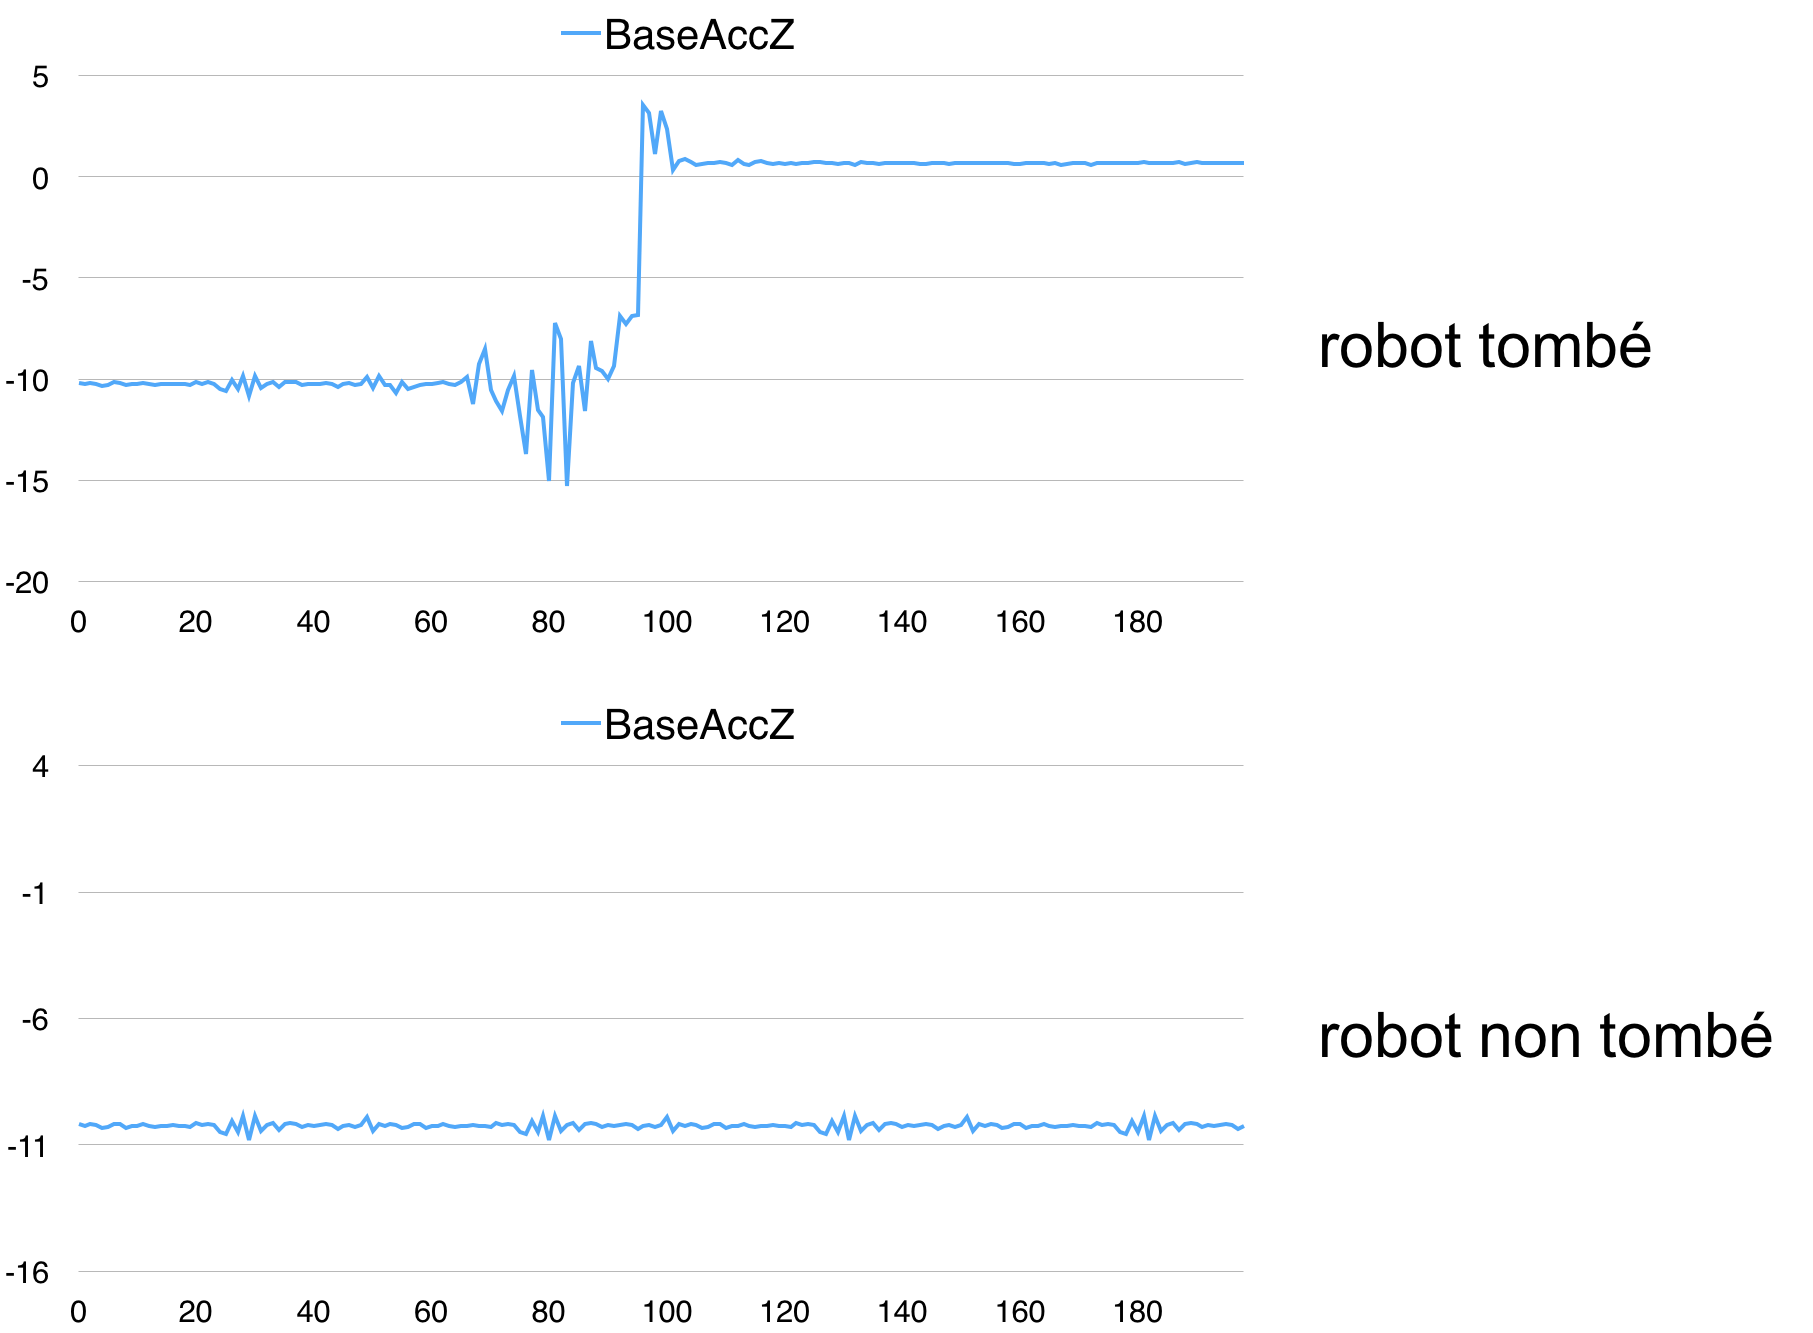
\includegraphics[width=12cm]{images/fall_not_fall.png}
	\caption[Formes caractéristiques de BaseAccZ en temps normal et en cas de chute]{Formes caractéristiques de BaseAccZ en temps normal et en cas de chute. On observe sur le graphe inférieur l'évolution de BaseAccZ lors d'un fonctionnement normal du robot. Sur le graphique supérieur, on observe l'évolution de BaseAccZ lorsque le robot chute. On remarque que celle-ci à la forme d'un échelon, centré sur l'instant où le robot tombe.}
	\label{fig:Formes caractéristiques de BaseAccZ en temps normal et en cas de chute}
\end{figure}

\begin{figure}[h]
	\centering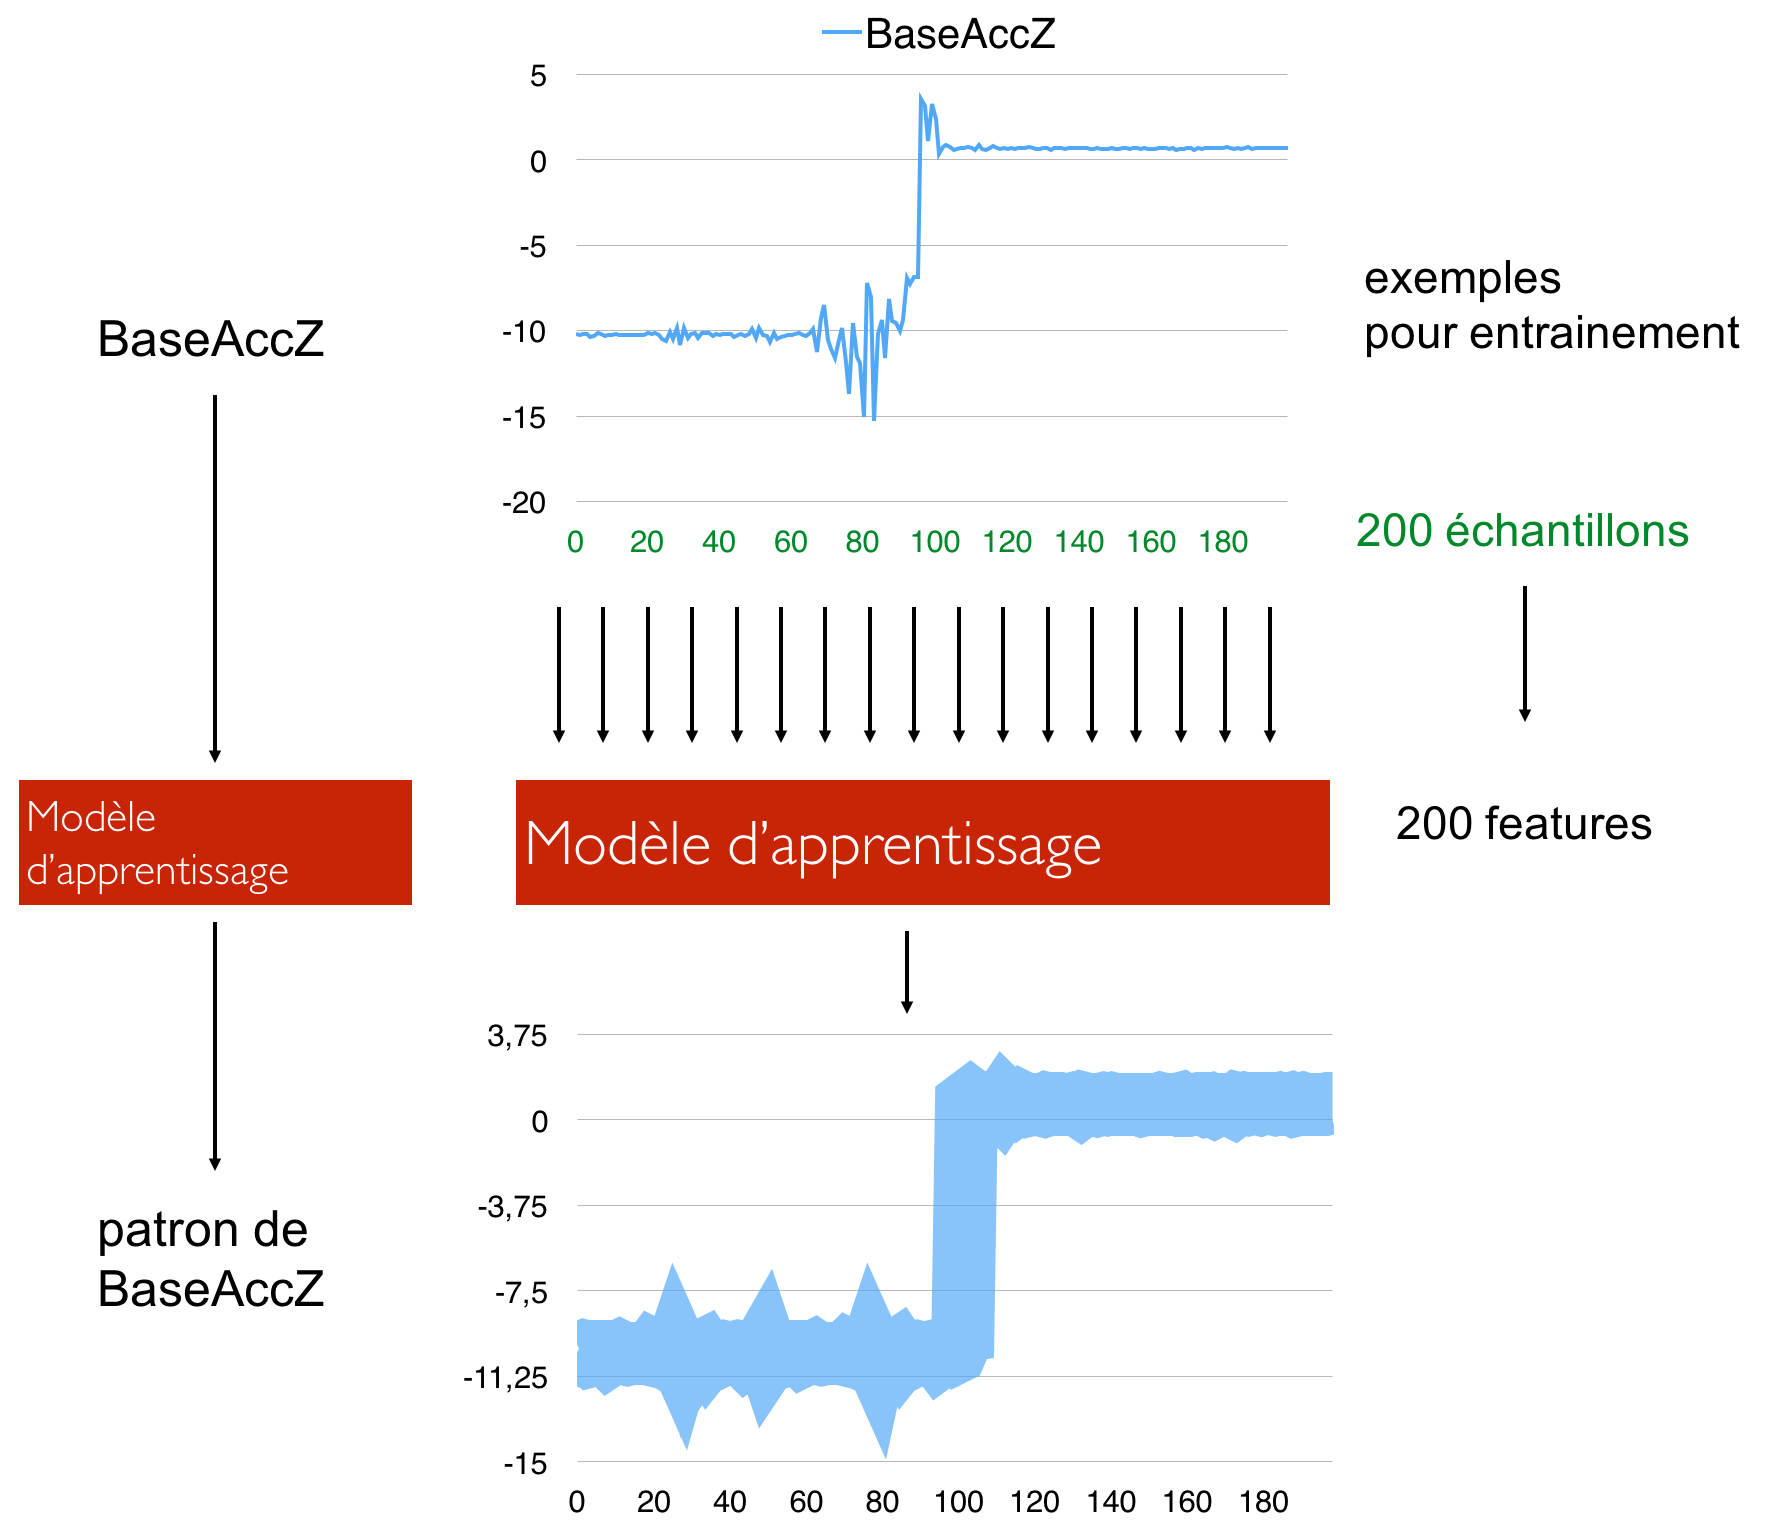
\includegraphics[width=12cm]{images/patron.png}
	\caption[Créer un patron caractéristique de la chute du robot]{Créer un patron caractéristique de la chute du robot. Chaque échantillon qui forment un exemple est considéré comme une entrée du système d'apprentissage, i.e. une feature. Entraîner l'algorithme à reconnaitre la forme de BaseAccZ, dans le case de robots tombés, revient à créer un patron de BaseAccZ qui caractérise la chute. L'entrainement s'effectue à partir de différents exemples de la feature BaseAccZ lorsque le robot tombe.}
	\label{fig:Créer un patron caractéristique de la chute du robot}
\end{figure}

\begin{figure}[h]
	\centering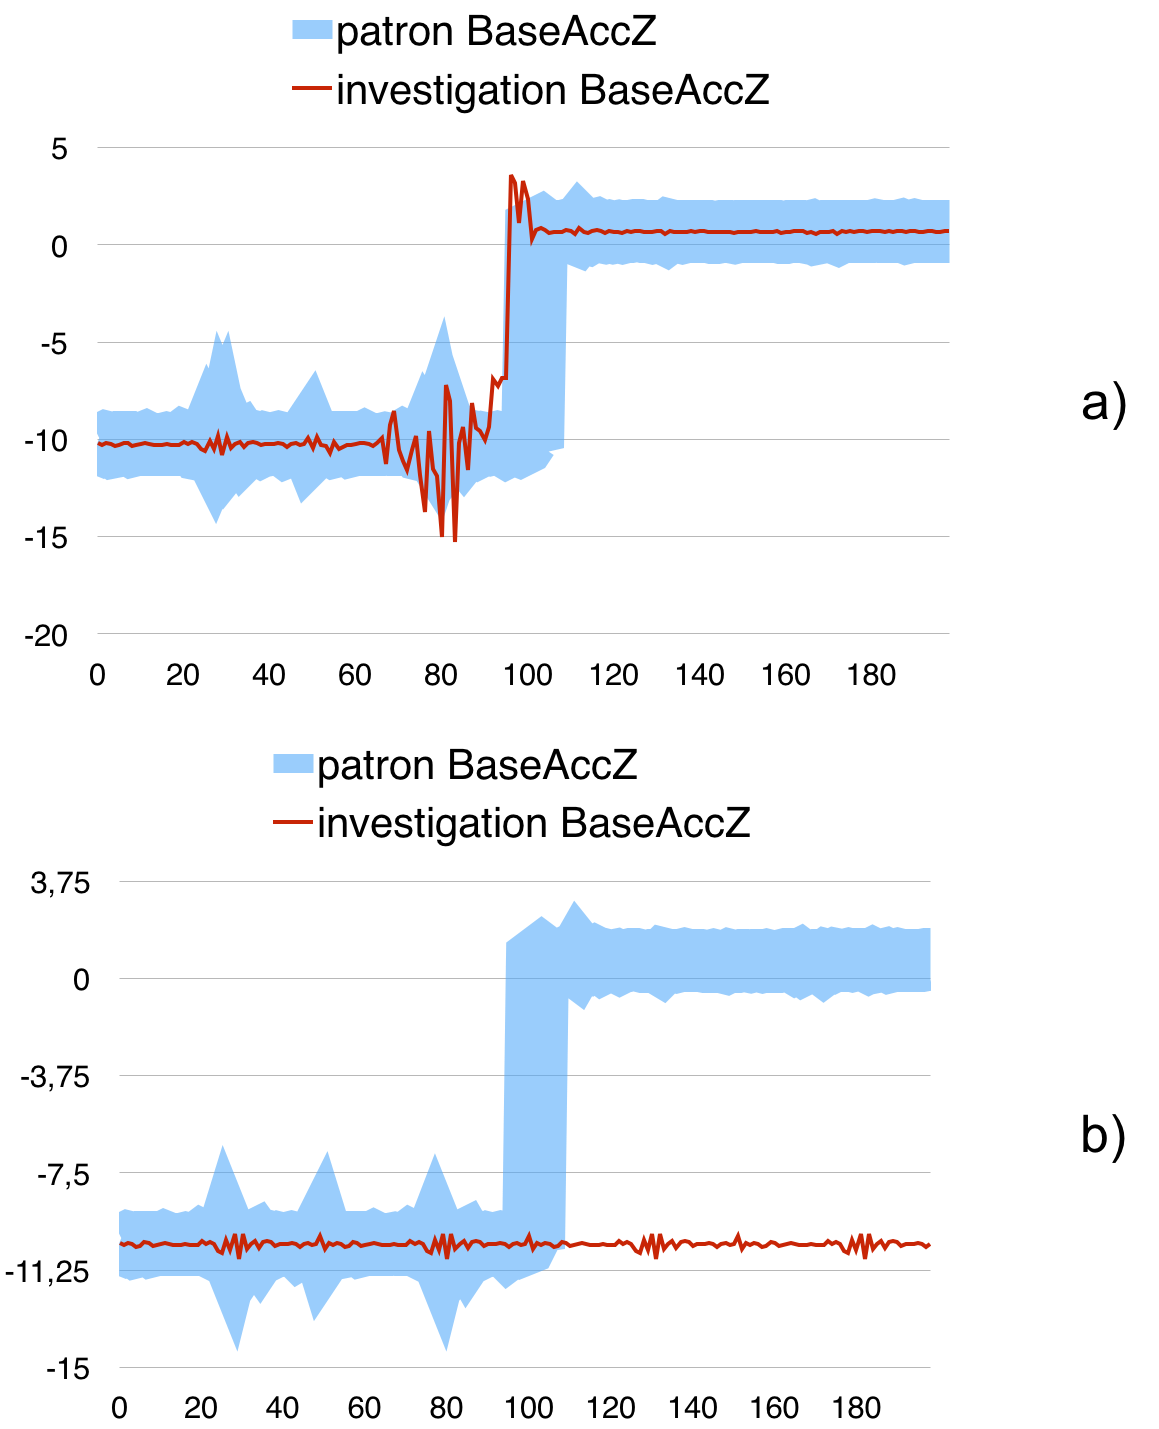
\includegraphics[width=12cm]{images/patron_comp.png}
	\caption[Détection d'une chute à partir du patron de BaseAccZ]{Détection d'une chute à partir du patron de BaseAccZ. Afin de savoir si l'exemple que l'on étudie est lié à une chute de robot ou non, on compare la valeur BaseAccZ du fichier log au patron caractéristique d'une chute de BaseAccZ. Sur le graphique supérieur, on observe que BaseAccZ est globalement contenu dans le patron, il s'agit donc d'un fichier log généré lors de la chute d'un robot. On observe en revanche sur le graphique inférieur que BaseAccZ n'est que \textbf{partiellement} incluse dans le patron. Il ne s'agit donc pas d'un exemple caractéristique d'une chute. }
	\label{fig:Détection d'une chute à partir du patron de BaseAccZ}
\end{figure}

Au vu des tests réalisés, cette méthode ne semble pas viable. En effet, comme on peut l'observer sur le graphique inférieur de la figure \ref{fig:Détection d'une chute à partir du patron de BaseAccZ}, même si la feature BaseAccZ n'est pas totalement inclue dans le patron, elle l'est \emph{partiellement} et ce sur pratiquement la moitié de son évolution. A cause de ce constat, l'algorithme considère dans certains cas un exemple comme caractéristique d'une chute alors qu'il ne l'est pas en réalité. Pour répondre à ce problème on propose que, plutôt que de créer un patron de la totalité de la courbe, on va seulement entraîner un algorithme à reconnaitre une certaine portion caractéristique de la courbe. Dans le cas de la détection d'une chute du robot, il s'agit du saut de valeur qui apparait sur la valeur de l'accélération en z du robot (BaseAccZ). On réalise de la reconnaissance de motifs. 

\subsection{Reconnaissance de motifs}
\label{Automatisation du processus d'investigation: Reconnaissance de motifs}
Au regard des études réalisées sur les différentes solutions qui s'offraient à nous pour la détection d'une root cause (cf. partie \ref{Automatisation du processus d'investigation: Reconnaissance de motifs: Différentes approches étudiées}), on souhaite à présent se tourner vers la reconnaissance de motif. 

\subsubsection{Principes généraux}
\label{Automatisation du processus d'investigation: Reconnaissance de motifs: Principes généraux}
D'une certaine manière, la reconnaissance de motif s'appuie sur une stratégie d'investigation proche de celle de l'Homme. On se place par exemple dans le cas où on souhaite déterminer la cause ayant entraîné la chute d'un robot. La cause correspond à la \emph{root cause} et la chute du robot à \emph{l'error name}. En tant qu'humain, on visualise et analyse les différentes courbes contenues dans le fichier log, généré lors de la détection de la chute au cours du Filtering Test. On observe alors les courbes de l'évolution de la position du senseur (clé HipPitchPositionSensorValue) et de l'actuateur (clé HipPitchPositionActuatorValue) de la hanche, figure \ref{fig:Évolution de la position du senseur et de l'actuateur de la hanche}. On remarque qu' à $t \approx 440 s$, le senseur se met à ne plus suivre la valeur de l'actuateur. L'étude réalisée partie \ref{Introduction:Expression du besoin:Exemple d'analyse d'une anomalie} nous \textbf{apprend} que cette particularité est la caractéristique d'un frottement des freins de la hanche. Ainsi, si on étudie ultérieurement un autre fichier log généré lors de la chute d'un robot et qu'on découvre ce motif, on en déduit aisément que le robot est également tombé à cause du frottement des freins de sa hanche. Plus on va observer de nouveaux cas, plus l'image que l'on a du motif caractéristique de cette \emph{root cause} va se préciser.\\
Dans le cadre du développement de notre algorithme, le principe est le même: on commence tout d'abord à apprendre la forme caractéristique de la root cause et une fois qu'on souhaite investiguer un nouveau fichier log, on compare ce motif caractéristique aux données du fichier. 

\begin{figure}[h]
	\centering\includegraphics[width=12cm]{images/HipPitch.png}
	\caption[Évolution de la position du senseur et de l'actuateur de la hanche]{Évolution de la position du senseur et de l'actuateur de la hanche.}
	\label{fig:Évolution de la position du senseur et de l'actuateur de la hanche}
\end{figure}

\paragraph{Apprentissage} La phase d'apprentissage s'appuie sur les principes évoqués en partie \ref{Automatisation du processus d'investigation: Reconnaissance de motifs: Différentes approches étudiées: Considérer chaque unité de temps comme une feature}. On considère que chaque échantillon (ou unité de temps) qui compose un exemple devient l'entrée de notre système d'apprentissage. A la différence qu'on considère qu'une partie de la courbe de nos exemples, le motif caractéristique. Par exemple, si on souhaite créer une nouvelle root cause "frottement des freins de la hanche", on sélectionnera sur chaque exemple le motif caractéristique de celle-ci (cf. figure \ref{fig:Créer un patron du motif caractéristique de la root cause "frottement des freins de la hanche"}). Le système d'apprentissage va donc uniquement apprendre le patron caractéristique du motif caractéristique et non de la courbe dans sa globalité. Les exemples devant être de la même taille on veille à sélectionner le même nombre d'échantillons pour chacun des motifs. On présente au système également des exemples ne contenant pas le motif, afin que l'algorithme bénéficie des deux types de labels pour son entrainement (root cause présente = 1, root cause non présente = 0).

\begin{figure}[h]
	\centering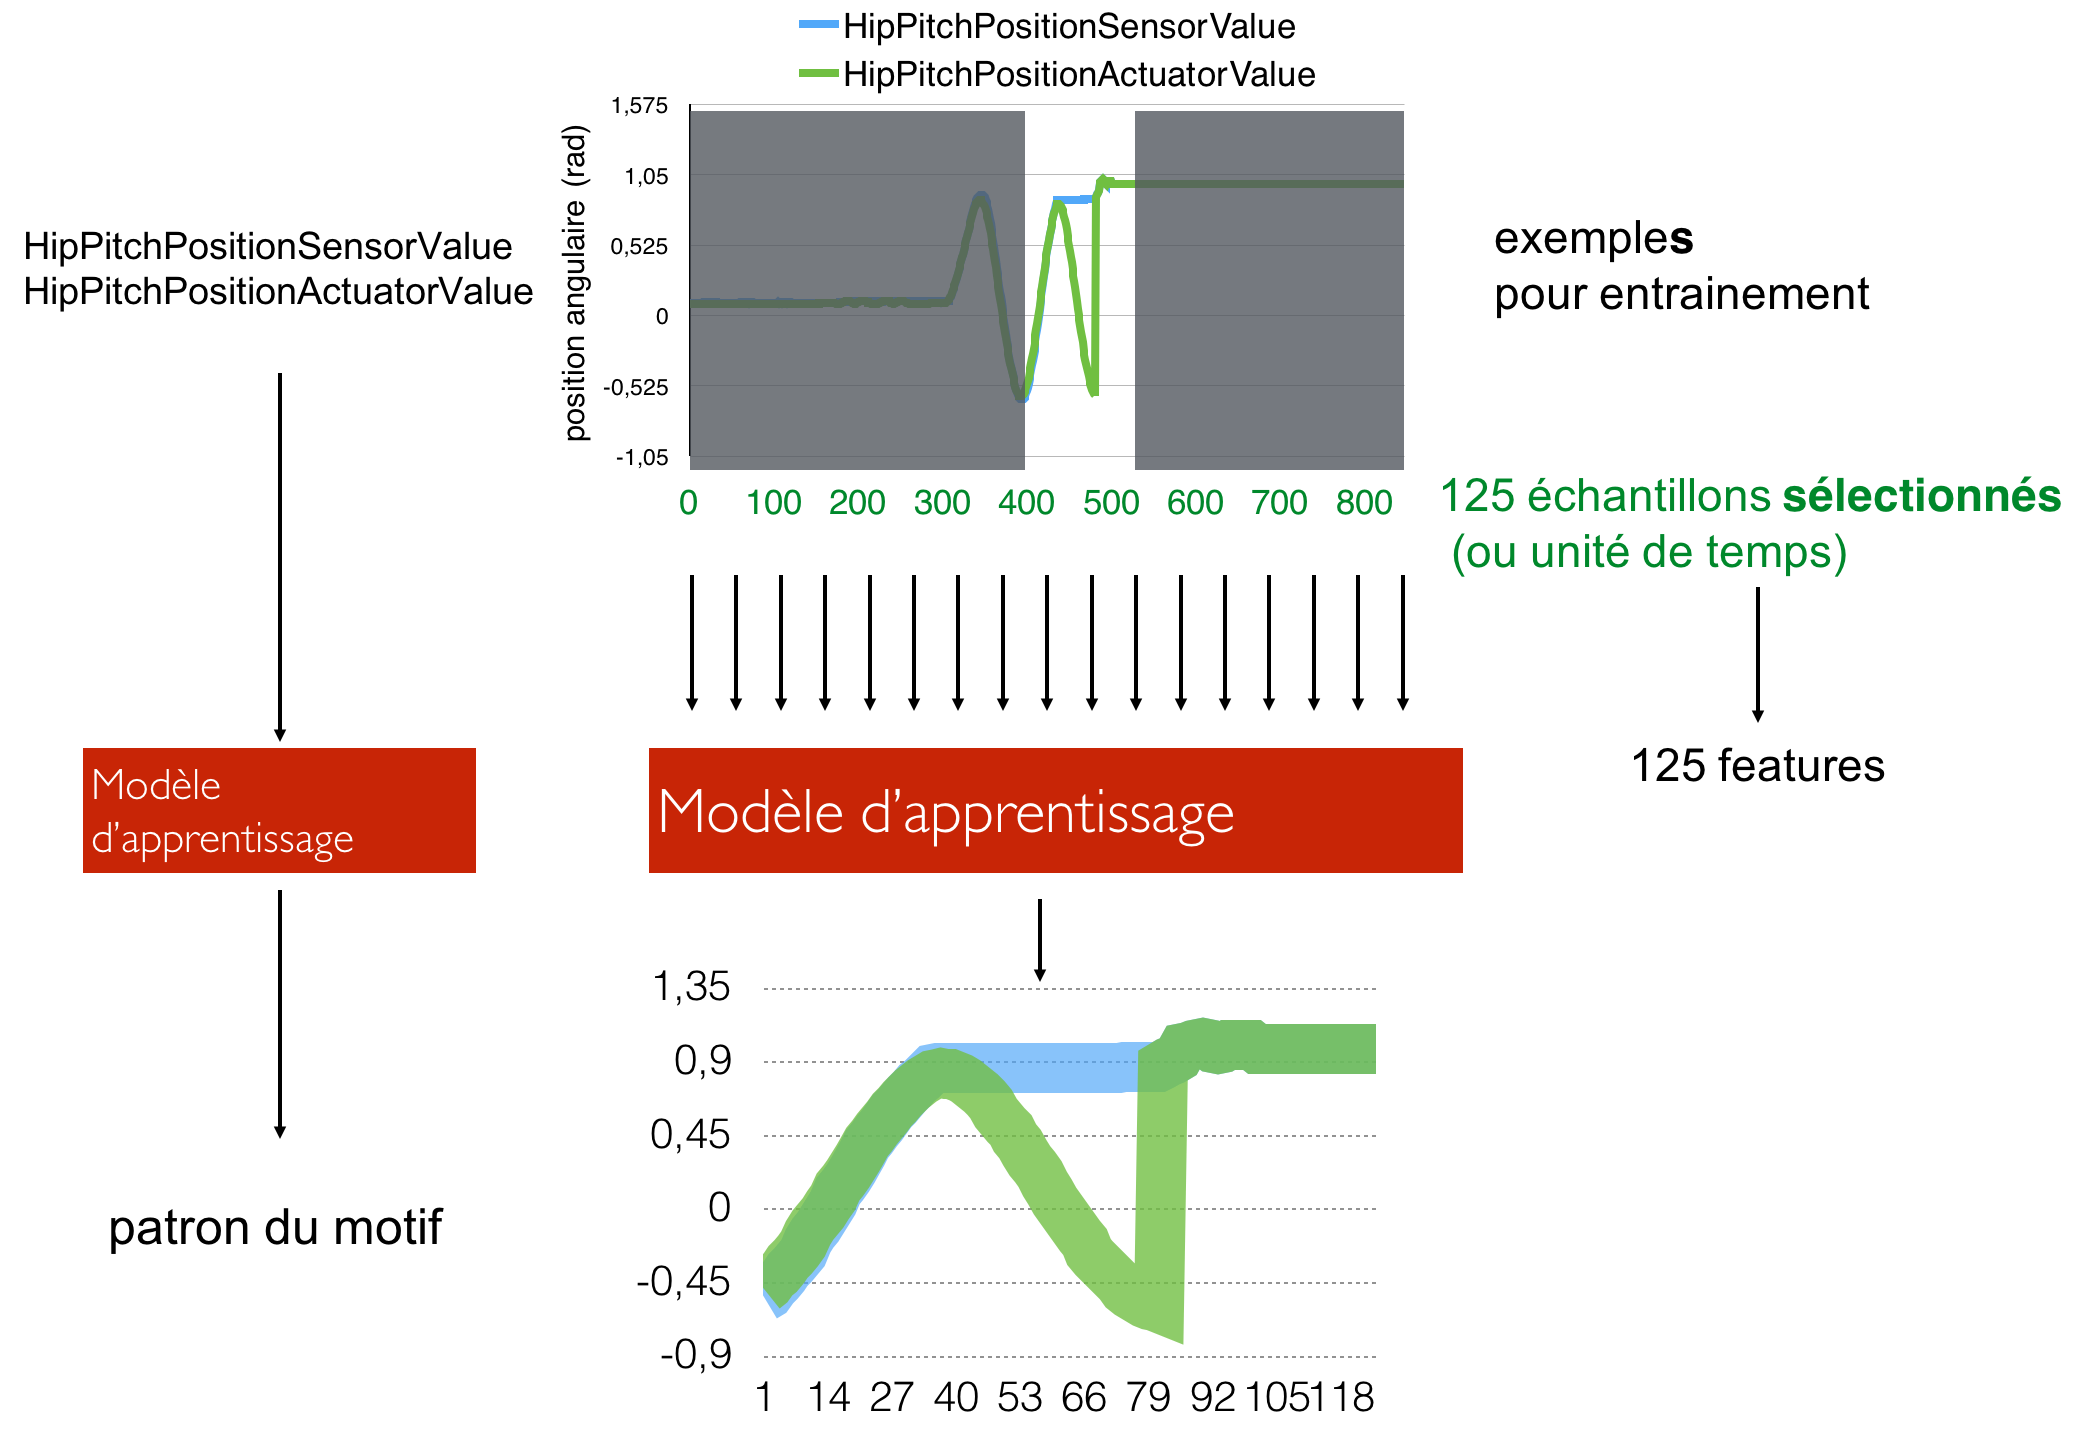
\includegraphics[width=14cm]{images/patron_motif.png}
	\caption[Créer un patron du motif caractéristique de la root cause "frottement des freins de la hanche"]{Créer un patron du motif caractéristique de la root cause "frottement des freins de la hanche". Chaque échantillon qui forment un motif est considéré comme une entrée du système d'apprentissage, i.e. une feature. Entraîner l'algorithme à reconnaitre le motif caractéristique formé par les courbes du HipPitchPositionSensorValue et HipPitchPositionActuatorValue revient à créer un patron caractéristique des deux features qui caractérise le frottement des freins de la hanche, dans le cadre de la chute robot. L'entrainement s'effectue à partir de différents exemples de motifs des deux features.}
	\label{fig:Créer un patron du motif caractéristique de la root cause "frottement des freins de la hanche"}
\end{figure}

\paragraph{Investigation}
Lorsque l'on souhaite investiguer un fichier pour déterminer la \emph{root cause} ayant entrainé l'apparition de l'\emph{error name} durant le Filering Test, on extrait la valeur des features du fichier log qui sont liées à la \emph{root cause}, puis on recherche le motif caractéristique. Pour cela, on découpe les courbes des features en plusieurs petits tronçons de la même taille que le motif caractéristique, et on les compare avec le motif caractéristique. Si ils sont globalement similaires au patron, on en déduit que la root cause a été détecté. Dans le cas contraire, on en déduit qu'elle n'a pas été détecté. En réalité, l'algorithme d'apprentissage automatique (SVM) nous retourne en sortie la probabilité avec laquelle le motif caractéristique a été détecté dans les courbes des features. On propose l'exemple d'investigation en figure \ref{fig:Balayage des features pour retrouver le motif caractéristique d'une root cause}).

\begin{figure}[h]
	\centering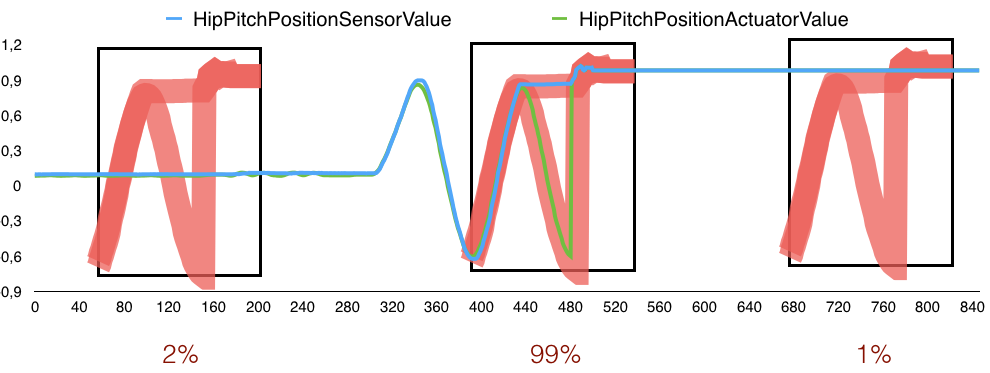
\includegraphics[width=12cm]{images/balayage_motif.png}
	\caption[Balayage des features pour retrouver le motif caractéristique d'une root cause]{Balayage des features pour retrouver le motif caractéristique d'une root cause. On observe que le premier et le dernier tronçon de la courbe des features HipPitchPositionSensorValue et  HipPitchPositionActuatorValue ne correspondent pas au motif caractéristique de la root cause "frottement des freins de la hanche". La probabilité en sortie du système est donc faible. Le deuxième tronçon correspond au motif caractéristique de la courbe, la probabilité en sortie du système est donc élevée.}
	\label{fig:Balayage des features pour retrouver le motif caractéristique d'une root cause}
\end{figure}

L'ensemble des probabilités en sortie des différents tronçons étudiés forment un courbe de probabilité. Si cette courbe dépasse un certain seuil, on considère la \emph{root cause} comme ayant été détectée. On propose la courbe de probabilité de la \emph{root cause} "frottement des freins de la hanche" en figure 	\ref{Automatisation du processus d'investigation}{fig:Courbe de probabilité de la root cause "frottement des freins de la hanche"}.

\begin{figure}[h]
	\centering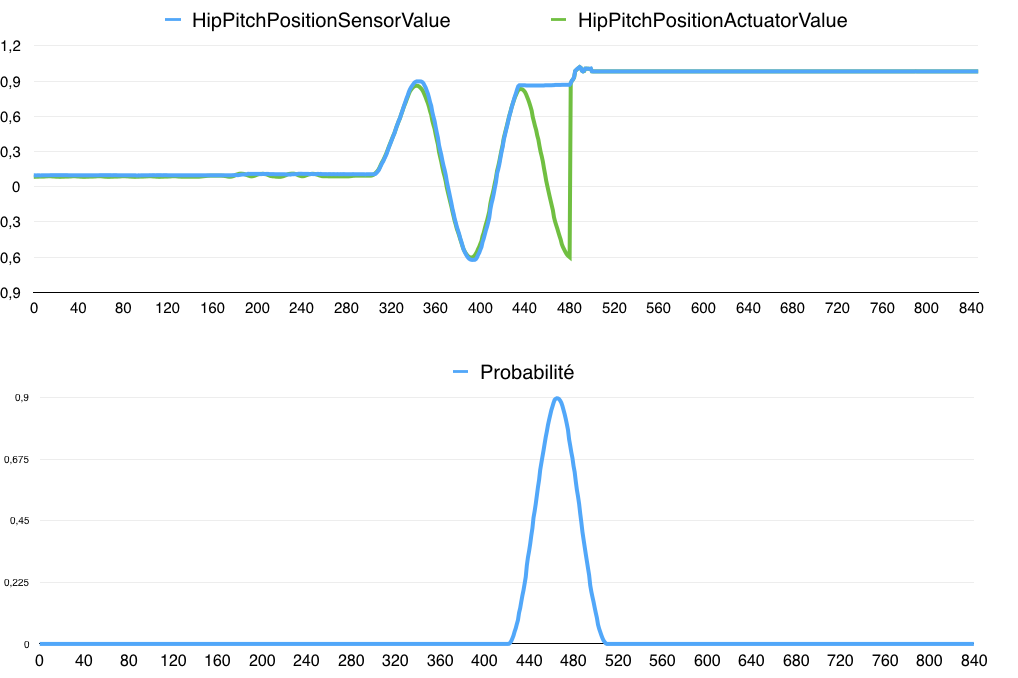
\includegraphics[width=12cm]{images/proba_motif.png}
	\caption[Courbe de probabilité de la root cause "frottement des freins de la hanche"]{Courbe de probabilité de la root cause "frottement des freins de la hanche".  On observe que lorsque l'on s'approche du motif caractéristique de la \emph{root cause}, la probabilité augmente fortement. Elle est au contraire faible sur les autres tronçons de la courbe.}
	\label{fig:Représentation de la répartition des exemples et des classes en fonction des features, approche fonctionnelle}
\end{figure}

\subsubsection{Exemples labellisés}
\label{Automatisation du processus d'investigation: Reconnaissance de motifs: Exemples labellisés}
Pour réaliser de l'apprentissage automatique, on rappelle que l'on a besoin d'exemples labellisés positifs (dans notre cas, le terme positif signifie des exemples de motifs caractéristiques de la \emph{root cause}) et des exemples labellisés négatifs (des exemples qui ne correspondent pas au motif caractéristique de la \emph{root cause}) . Ces exemples forment alors des classes. Dans le cadre de la \emph{root cause} "frottement des freins de la hanche", on peut visualiser l'ensemble de ces exemples et ces classes dans un repère construit à partir des features "position du senseur de la hanche" (clé HipPitchPositionSensorValue) et "position de l'actuateur de la hanche" (clé HipPitchPositionActuatorValue)

\subsubsection{Représentation des données}
\label{Automatisation du processus d'investigation: Reconnaissance de motifs: Représentation des données}
On souhaite représenter de manière intuitive la répartition des exemples et des classes en fonction des features. Contrairement à la visualisation conceptuelle des données proposée en partie \ref{Automatisation du processus d'investigation: Achitecture High Level du système proposé: Les exemples: Représentation des exemples et des classes}, on propose ici une représentation plus fonctionnelle (proche du fonctionnement de notre système d'automatisation). \\
Chaque échantillon qui compose le motif caractéristique d'une \emph{root cause}, contenu dans la feature d'un exemple (e.g. "HipPitchPositionSensorValue") devient donc elle même une feature (i.e. une entrée) du système d'apprentissage de l'algorithme SVM \ref{fig:Créer un patron caractéristique de la chute du robot}). Par exemple, on se place de nouveau dans le cas de la \emph{root cause} "frottement des freins de la hanche". Si on s'intéresse aux features "HipPitchPositionSensorValue" et "HipPitchPositionSensorValue" et que l'on considère que le motif caractéristique à une taille de 125 échantillons, on aura donc 250 features en entrée de l'apprentissage. Cela signifie que si l'on souhaite représenter visuellement la répartition des exemples et des classes en fonction des features, on aurait un repère composé de 250 dimensions. On choisi au hasard deux de ses 250 dimensions et on les représente sur le repère figure 	\ref{fig:Courbe de probabilité de la root cause "frottement des freins de la hanche"} .

\begin{figure}[h]
	\centering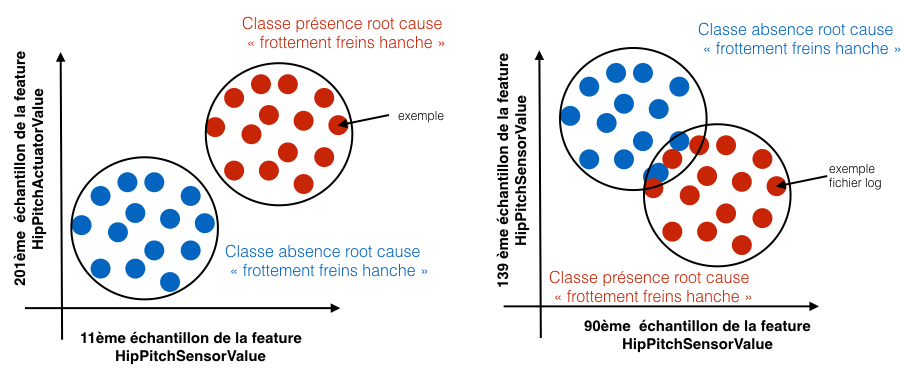
\includegraphics[width=12cm]{images/classes_sys.png}
	\caption[Représentation de la répartition des exemples et des classes en fonction des features,  approche fonctionnelle]{Représentation de la répartition des exemples et des classes en fonction des features. On a représenté ici deux graphiques dont chacun exprime la valeur des exemples en fonction de deux features choisies aléatoirement. Chaque feature correspond à un échantillon parmi les 250 qui composent chaque motif caractéristique de la \emph{root cause} "frottement des freins de la hanche".}
	\label{fig:Courbe de probabilité de la root cause "frottement des freins de la hanche"}
\end{figure}



\section{Performances de la solution}
\label{Automatisation du processus d'investigation: Performances de la solution}
Une fois l'architecture du système définie, on souhaite mesurer les performances de l'algorithme.

\subsection{Optimisation des paramètres du SVM}
\label{Industrialisation du produit: Performances de la solution:Optimisation des paramètres du SVM}
La prise de décision de l'algorithme du SVM peut être contrôlée via deux paramètres: C et gamma.
\begin{description}
	\item [C] Le paramètre C permet de modifier la valeur de la marge du SVM. \\
	Une valeur élevée du paramètre cherchera par exemple à optimiser la classification de chaque exemple en entrée, i.e. à trouver une ligne de décision permettant de classer au mieux chaque exemple. Cette optimisation de la classification se fait cependant au préjudice de la taille de la marge, qui sera réduite. \\
	Une valeur plus élevée de C permet au contraire d'optimiser la taille de la marge (i.e. la maximiser autant que possible), au préjudice de la classification des exemples.
	\item [gamma] Intuitivement, le paramètre gamma définit dans quelle mesure l'influence d'un exemple affecte la ligne de décision et la marge. Il peut être considéré comme l'inverse du rayon d'influence des échantillons sélectionnés par le modèle, en tant que vecteurs de support.
\end{description}

Afin de déterminer la meilleure combinaison de valeurs des deux paramètres, on calcule les \emph{courbes de validation}. Cela consiste à faire varier chacun des deux paramètres sur une plage de données et à calculer la précision de l'algorithme pour chaque valeur. On conserve ensuite la valeur optimale. 

 \paragraph{Exemple}
 On soumet en figure \ref{fig:Courbes de validation} les courbes de validation de la couche \emph{root cause} "frottement des freins de la hanche". 

 \begin{figure}[h]
 	\centering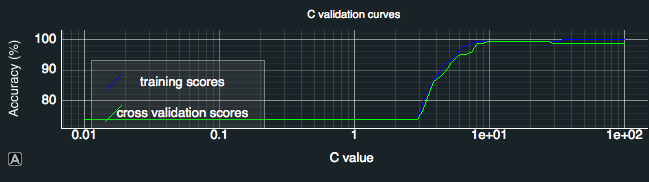
\includegraphics[width=12cm]{images/courbe_validation_c.png}
 	\caption[Courbes de validation du paramètre C]{Courbes de validation du paramètre C, pour la couche \emph{root cause} "frottement des freins de la hanche".}
 	\label{fig:Courbes de validation du paramètre C}
 \end{figure}
 
  \begin{figure}[h]
  	\centering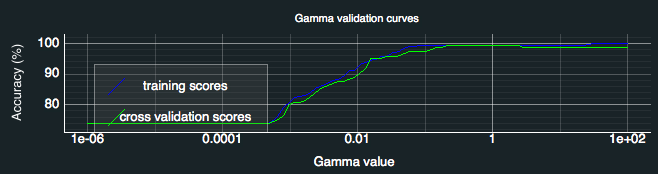
\includegraphics[width=12cm]{images/courbe_validation_gamma.png}
  	\caption[Courbes de validation du paramètre gamma]{Courbes de validation du paramètre gamma, pour la couche \emph{root cause} "frottement des freins de la hanche".}
  	\label{fig:Courbes de validation du paramètre gamma}
  \end{figure}
  
\subsection{Matrices de confusion}
\label{Industrialisation du produit: Performances de la solution:Matrices de confusion}
Au début du processus, on sépare la base de données d'exemples en deux groupes : le \emph{training set} et \emph{test set}. Le premier jeu sert à entraîner l'algorithme SVM et l'autre permet d'en tester les performances. On rappelle que chaque exemple est labellisé, i.e. on connait  la sortie à laquelle ils sont corrélés (dans le cas de notre problématique, les labels étant \emph{root cause} présente ou non présente) 
\newline

Pour tester l'algorithme : 
\begin{enumerate}
	\item On commence par entrainer l'algorithme d'apprentissage automatique (SVM) à partir des exemples du \emph{training set}
	\item Une fois l'algorithme entraîné, on analyse chacun des exemples du \emph{test set}
	\item On compare ensuite la sortie prédite par l'algorithme et la sortie réelle (i.e. le label associé à chaque exemple). 
\end{enumerate}

Ainsi, on est capable de calculer le nombre de fois que l'algorithme a correctement prédit la sortie et lorsqu'il ne l'a pas fait. Ces résultats peuvent être exprimés sous la forme d'une matrice de confusion. Chaque colonne de la matrice représente le nombre d'occurrences d'une classe réelle (le label), tandis que chaque ligne représente le nombre d'occurrences de la classe prédite. Un des intérêts de la matrice de confusion est qu'elle montre rapidement si le système parvient à classifier correctement. 

\begin{table}[H]
	\centering
	\begin{tabular}{| c | c | c | c |}
		\hline
		\multicolumn{2}{|c|}{}  & \multicolumn{2}{|c|}{Classe réelle } \\
		\cline{3-4}
		\multicolumn{2}{|c|}{}  & Vrai & Faux \\
		\hline
		\multirow{2}*{Classe prédite} & Vrai & TP & FP \\
		\cline{2-4}
		& Faux & FN & TN \\
		\hline
	\end{tabular}
	\caption[Matrice de confusion]{Matrice de confusion}
	\label {tab:Matrice de confusion}
\end{table}

Avec : 
\begin{itemize}
	\item TP = True positive (en français vrai positif) correspond au nombre de résultats prédits positifs, là où ils étaient effectivement positifs.
	\item TN = True negative (en français vrai négatif) correspond au nombre de résultats prédits négatifs, là où ils étaient effectivement négatifs.
	\item FP = False positive (en français faux positif) correspond au nombre de résultats prédits positifs, là où ils étaient étaient en réalité négatifs.
	\item FN = False negative ( en français faux négatif) correspond au nombre de résultats prédits négatifs, là où ils étaient étaient en réalité positifs.
\end{itemize}
 
A partir de ces résultats, il est possible de déterminer la précision de l'algorithme:
\begin{equation}
	\text{accuracy}= \frac{TP + TN}{TP + TN + FP + FN}
	\label{accuracy}
\end{equation}
 
 \paragraph{Exemple}
 On soumet ici la matrice de confusion de la couche \emph{root cause} "frottement des freins de la hanche". On remarque que la valeur $C = 10$ optimise le mieux la précision de l'algorithme d'apprentissage. On remarque également que la valeur $gamma \approx 0.2$ optimise le mieux la précision de l'algorithme d'apprentissage.
 
\begin{table}[H]
	\centering
	\begin{tabular}{| c | c | c | c |}
		\hline
		\multicolumn{2}{|c|}{}  & \multicolumn{2}{|c|}{Classe réelle } \\
		\cline{3-4}
		\multicolumn{2}{|c|}{}  & Vrai & Faux \\
		\hline
		\multirow{2}*{Classe prédite} & Vrai & 45 & 0 \\
		\cline{2-4}
		& Faux & 0 & 15 \\
		\hline
	\end{tabular}
	\caption[Matrice de confusion de la root cause "frottement des freins de la hanche"]{Matrice de confusion de la root cause "frottement des freins de la hanche"}
	\label {tab:Matrice de confusion de la root cause "frottement des freins de la hanche"}
\end{table}

On observe qu'il n'y a aucun faux négatif et faux positif. Cela signifie que pour chaque exemple du \emph{test set}, l'algorithme à parfaitement prédit la sortie, i.e. qu'il a su à chaque fois détecter correctement si la root cause "frottement des freins de la hanche" était présente ou non dans le fichier log. D'après l'équation \ref{accuracy}, la précision de l'algorithme SVM de cette couche \emph{root cause} est donc de $100\%$.
 
\subsection{Courbes d'apprentissage}
\label{Industrialisation du produit: Performances de la solution:Courbes d'apprentissage}
Les courbes d'apprentissage représente la précision de l'algorithme d'apprentissage en fonction du nombre d'exemples utilisés dans le \emph{training set} et le \emph{test set}. Grâce à ces tracés, on est en mesure de déterminer la qualité de notre algorithme d'apprentissage et de la base de données d'exemples, de manière visuelle et intuitive. 
\begin{itemize}
	\item Si la distance entre les deux courbes est importante entre les deux courbes à la fin du graphe, cela signifie que l'on a pas assez d'exemples pour l'entraînement de l'algorithme d'apprentissage. On dit que l'algorithme a une \emph{variance} trop élevée. 
	\item Si la valeur de convergence des deux courbes (précision) n'est pas assez élevé, cela signife que notre algorithme n'est pas suffisamment performant. On dit qu'elle a un \emph{bias} trop élevé. Pour résoudre ce problème, on peut par exemple augmenter le nombre de features en entrée. Dans le cas de notre système, cela signifie augmenter la largeur des motifs caractéristiques d'une \emph{root cause}.
\end{itemize}

\paragraph{Exemple}
On soumet en figure \ref{fig:Courbes d'apprentissage} les courbes d'apprentissage de la couche \emph{root cause} "frottement des freins de la hanche". On observe que les deux courbes convergent jusqu'à pratiquement se confondre. Cela signifie que la \emph{variance} de l'algorithme est très faible et donc que le nombre d'exemples utilisés pour l'apprentissage de l'algorithme est suffisant. De plus, la valeur de convergence est aux alentours de 98\%, ce qui signifie que le \emph{bias} de l'algorithme est faible. On peut donc dire que les performances de l'algorithme de la couche \emph{root cause} "frottement des freins de la hanche" sont bonnes. 

\begin{figure}[h]
\centering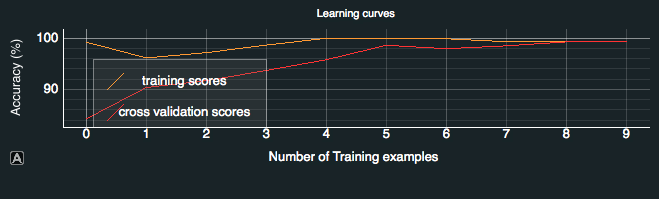
\includegraphics[width=12cm]{images/courbe_apprentissage.png}
\caption[Courbes d'apprentissage]{Courbes d'apprentissage de la couche \emph{root cause} "frottement des freins de la hanche".}
\label{fig:Courbes d'apprentissage}
\end{figure}
\chapter{Industrialisation du produit}
\label{Industrialisation du produit}
\thispagestyle{fancy}
Une fois le processus fonctionnel de notre système défini, on l'industrialise. Cela signifie que l'on crée un ensemble d'outils permettant de l'utiliser de la manière la plus simple possible et en répondant au mieux à la problématique initiale. \\
On soumet deux types d'outils: l'API, qui permet d'utiliser le système d'automatisation, et les outils graphiques, qui accompagnent l'usage de l'API et offrent à l'utilisateur un moyen d'interagir avec le programme.  

\section{API}
\label{Industrialisation du produit: API}
L'API que l'on propose est composée de 3 modules :
\begin{description}
	\item [data base] Permet de gérer le stockage et la lecture des données nécessaires à l'exécution des algorithmes d'apprentissage. Deux types de fichiers y sont sauvegardés : les fichiers logs, qui fournissent l'ensemble des exemples permettant d'entraîner le SVM et les fichiers générés par l'algorithme lors de son apprentissage.
	\item [data set] Permet de pré-traiter les exemples utilisés pour l'apprentissage.
	\item [machine learning] Permet de créer un algorithme d'apprentissage, de l'entraîner et de l'utiliser pour investiguer la \emph{root cause} pour laquelle il a été créé.
\end{description}

La librairie utilise le langage de programmation Python \cite{Python}. \\

\subsection{Pré-traitement des données}
\label{Industrialisation du produit: API: Pré-traitement et traitement des données}
Le module "Data set" de l'API permet de pré-traiter les exemples et de les structurer, afin de pouvoir entraîner le SVM. 
Le pré-traitement est composé de 5 étapes.
\begin{description}
	\item [Lecture] Consiste à lire les données contenues dans le fichier log. 
	\item [Échantillonnage] Les fichiers logs générés par MEIGUI lors du déroulement du Filtering Test n'ont pas forcement tous la même période d'échantillonnage. Cela signifie que les exemples que l'on souhaite utiliser pour l'entraînement ne font pas tous la même taille. Or, les spécificités des fonctions de la librairie Scikit-learn utilisées pour l'entraînement nécessite que celles-ci aient le même nombre d'échantillons. Pour cette raison, on échantillonne les données extraites des fichiers logs ou le même nombre d'échantillons. Si le nombre d'échantillons contenus dans le fichier log est inférieur au nombre d'échantillons fixé par l'échantillonnage, on effectue un sur-échantillonnage, quand celui-ci n'altère les données. 
	\item [Selection des motifs] Au regard de l'architecture fonctionnelle que l'on a définie en partie \ref{Automatisation du processus d'investigation: Achitecture High Level du système proposé}, on doit extraire les motifs caractéristiques d'une root cause dans chaque exemple utilisé. Pour cela, une sélection manuelle du motif est réalisée en amont via une interface graphique (c.f. \ref{Industrialisation du produit: Présentation des outils: Outils graphiques}). A partir des informations retournées par l'IHM (Interface Homme Machine), on est en mesure de sélectionner les portions des exemples qui correspondent aux motifs. On rappelle que l'on sauvegarde également des morceaux de la courbe ne contenant pas de motif caractéristique d'une \emph{root cause}. Cette étape permet également de labelliser les exemples, i.e. indiquer si le motif sélectionné correspond à un motif caractéristique de la \emph{root cause}.
	\item [Déroulement des données] On déroule ensuite les données pour réaliser de la reconnaissance de motifs avec plusieurs features (cf. partie \ref{Automatisation du processus d'investigation: Étendre le problème à plusieurs dimensions}), i.e. que l'on place chacune des colonnes de notre matrice d'exemples les en dessous des autres. On obtient en sortie un vecteur. 
	\item [Tri des données] Enfin, pour mesurer les performances de notre algorithme (c.f. partie \ref{Automatisation du processus d'investigation: Performances de la solution}), on sépare notre base de données d'exemples en deux groupes: le \emph{training set} et le \emph{test set}. Le premier sera utilisé pour entraîner notre algorithme, le deuxième pour le tester. 
\end{description}

\subsubsection{Sélection des motifs}
\label{Industrialisation du produit: API: Sélection des motifs}
Comme étudié en partie \ref{Automatisation du processus d'investigation: Reconnaissance de motifs}, la reconnaissance de motifs passe par la sélection des motifs caractéristiques de la root cause que l'on souhaite détecter, dans chaque exemple de notre base de données. Elle s'accompagne également de  la sélection de sections de la courbe ne présentant pas ce motif afin de pouvoir réaliser l'apprentissage de l'algorithme de manière optimale( c.f. partie \ref{Automatisation du processus d'investigation: Difficultés notoires rencontrées}).\\
 Chaque motif sélectionné doit avoir la même taille i.e. le même nombre d'échantillons pour pouvoir réaliser l'entrainement. Cette taille dépend de la largeur globale du motif caractéristique et est déterminée par l'utilisateur lors de l'utilisation de l'interface graphique présentée partie \ref{Industrialisation du produit: Outils graphiques: Pattern selection} .   

\subsubsection{Format des données de sortie}
\label{Industrialisation du produit: API: Format des données de sortie}
On présente dans le tableau \ref {tab: Structure de la base de données d'exemples après prétraitement} la structure des données en sortie du pré traitement des données. On a deux vecteur : un contenant les exemples de motifs et un deuxième contenant le label associé à chaque motif. Le label 1 signifie que le motif correspond à un motif caractéristique de la \emph{root cause} ; 0 signifie que le motif ne correspond pas à un motif caractéristique de la \emph{root cause}. 
\begin{equation}
\begin{blockarray}{cc}
exemples & labels \\
\begin{block}{[c][c]}
exemple_1 &  1 \\
exemple_2 & 0 \\
exemple_3 & 0 \\
exemple_4 & 1 \\
... & ... \\
exemple_m & 0 \\
\end{block}
\end{blockarray}
\label {tab: Structure de la base de données d'exemples après prétraitement}
\end{equation}
On retrouve cette structure pour chaque \emph{set} (i.e. \emph{training set} et \emph{test set}). \\
Chaque exemple correspond à une liste qui contient l'ensemble des échantillons contenus dans un motif.

\subsection{Module Marchine Learning}
\label{Industrialisation du produit:  API: Le module Machine Learning}
Le module Machine Learning s'appuie sur l'utilisation de scikit-learn \cite{ScikitLearn}. Il s'agit d'une bibliothèque Open Source développée par l'INRIA (Institut National de Recherche en Informatique et en Automatique \cite{INRIA}). Elle propose de nombreux outils qui permet de réaliser de la classification (régression logistique, SVM), de la régression (SVR, régression linéaire) et du clustering (i.e. apprentissage non supervisé). On l'utilise dans le cadre ne notre projet pour réaliser de classification (i.e. apprentissage supervisé) en utilisant l'algorithme d'apprentissage automatique SVM. Elle est également utilisée afin de construire le \emph{training set} et le \emph{test set} et déterminer les performances de l'algorithme.




\section{Outils graphiques}
\label{Industrialisation du produit: Outils graphiques}
On présente ici les différents outils graphiques qui permettent de réaliser la construction d'une nouvelle couche root cause (i.e. un nouvel algorithme pour détecter une \emph{root cause}), d'investiguer une \emph{error name} et d'obtenir des informations sur les performances de l'algorithme. 

\subsection{Pattern selector}
\label{Industrialisation du produit: Outils graphiques: Pattern selection}
Cet outil graphique permet de sélectionner les motifs contenus dans chaque exemple du \emph{training set} lors la phase de pré-traitement des exemples.  Il permet également  de labelliser les exemples. \\
Il est formé de trois parties:
\begin{itemize}
	\item La première partie (encadré vert de la figure \ref{fig:Interface graphique du pattern selector}) nous fournie des informations sur l'état actuel du pré-traitement des données : la taille du motif sélectionné, le nom de l'exemple étudié et le nombre d'exemples restant à traiter. 
	\item La seconde partie (encadré rouge de la figure  \ref{fig:Interface graphique du pattern selector}) affiche les features de l'exemple actuellement étudiée. Dans le cas de la figure  \ref{fig:Interface graphique du pattern selector}, on réalise par exemple l'entraînement de l'algorithme pour que celui-ci puisse reconnaître le motif caractéristique de la root cause "frottement des freins de la hanche". La région en rouge permet de sélectionner le motif qui nous intéresse.
	\item La dernière partie (encadré bleu de la figure  \ref{fig:Interface graphique du pattern selector}) est une succession de boutons qui permettent à l'utilisateur d'interagir avec les différents exemples. De gauche à droite :   
	\begin{itemize}
		\item Le  bouton "Previous" permet de revenir à l'exemple précédent.
		\item Le bouton "Found" permet d'indiquer au système que le motif est présent sur l'exemple étudié, et qu'il a bien été sélectionné grâce à la région de sélection. Cela revient à labelliser l'exemple (Y = 1, c.f. partie \ref{Industrialisation du produit: API: Format des données en sortie du pré-traitement}). Le prochain exemple à étudier s'affiche.
		\item Le bouton "Not Found" permet d'indiquer au système que le motif n'est pas présent sur l'exemple étudié. Cela revient à labelliser l'exemple (Y = 0, c.f. partie \ref{Industrialisation du produit: API: Format des données en sortie du pré-traitement}). Le prochain exemple à étudier s'affiche.
		\item Le bouton en forme d'œil ouvert permet d'activer le mode étendu (c.f. figure \ref{fig:Interface graphique du pattern selector en mode étendu}).
	\end{itemize} 
\end{itemize} 

\begin{figure}[H]
	\centering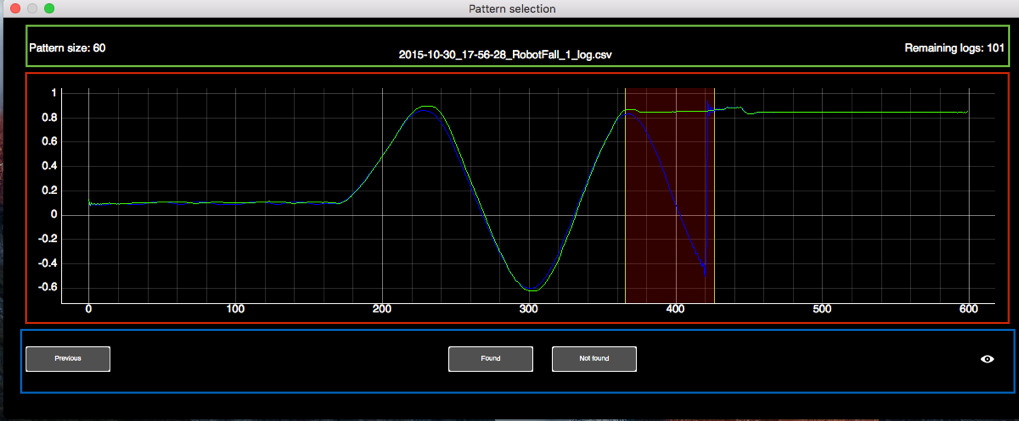
\includegraphics[height=6.4cm]{images/pattern_selector.png}
	\caption[Interface graphique du pattern selector]{Interface graphique du pattern selector.}
	\label{fig:Interface graphique du pattern selector}
\end{figure}

\subsubsection{Région de sélection}
\label{Industrialisation du produit: Outils graphiques: Pattern selection: La région de sélection}
La région de sélection permet de sélectionner le motif caractéristique d'une \emph{root cause} dans chaque exemple où celui-ci se présente. \\
 Il est possible d'augmenter la taille de celui-ci si le besoin est présent. Par exemple, imaginons que l'on sélectionne sur le premier exemple un motif, dont la taille est de 60 échantillons. On clique sur le bouton "Found" et un nouvel exemple s'affiche. Celui-ci contient également le motif caractéristique de la \emph{root cause} que l'on apprend. Cependant, ce dernier est plus large de 10 échantillons. Il est alors possible d'étendre la région de sélection pour pouvoir sélectionner l'ensemble de ce nouveau motif. Cependant, l'ensemble des exemples devant avoir la même taille (même nombre d'échantillons), on modifie la taille des motifs précédemment sélectionnés. Dans le cas de notre exemple, on augmente la taille du motif précédent de 5 échantillons de chaque côté. \\
Il n'est cependant pas possible de réduire la taille d'un motif, pour ne pas perdre des données sur les exemples précédemment sélectionnés. 

\subsubsection{Mode étendu}
\label{Industrialisation du produit: Outils graphiques: Pattern selection: Mode étendu}
Il existe certains cas où les valeurs de deux features étudiées sont trop éloignées l'une de l'autre pour pouvoir être visualisé de manière correct. Pour cela, on peut basculer l'IHM en mode étendu, ce qui permet d'afficher chacune des features dans un graphique séparé. La région de sélection est commune aux différents graphe, i.e. sa taille et sa position est contrôlée via le graphique principal et se répercute sur les graphitiques du mode étendu (c.f. figure \ref{fig:Interface graphique du pattern selector en mode étendu})

\begin{figure}[H]
	\centering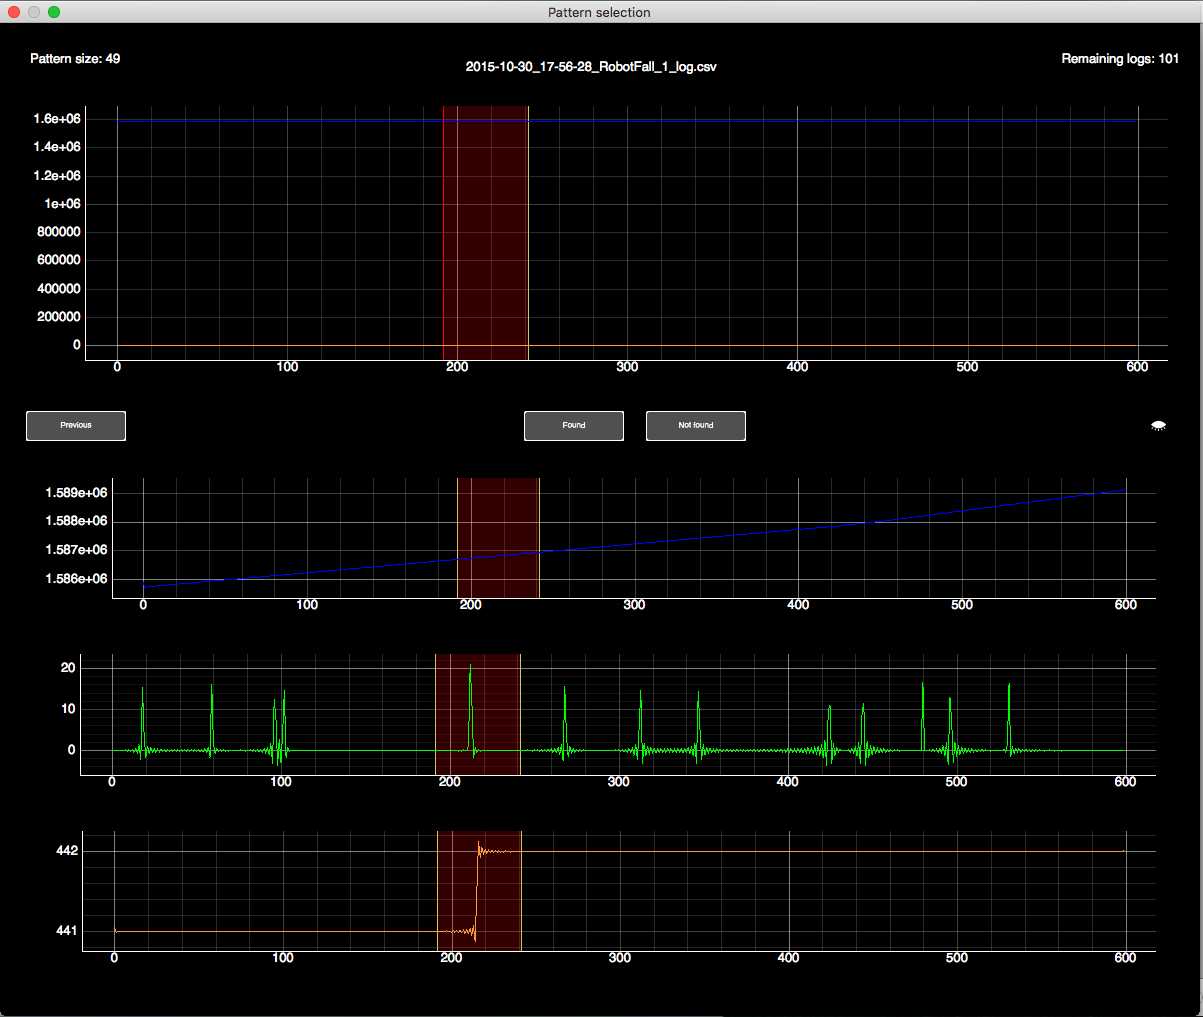
\includegraphics[height=9cm]{images/pattern_selector_ext.png}
	\caption[Interface graphique du pattern selector en mode étendu]{Interface graphique du pattern selector en mode étendu. On observe sur ce graphiques les trois features BackPlateformAck, BackPlateformNack et BackPlateformError du premier exemple. On remarque que l'affichage sur le graphique principal n'est pas clair. Le mode étendu permet d'afficher chacune des features. La région de sélection est commune aux trois graphiques (même position, même taille).}
	\label{fig:Interface graphique du pattern selector en mode étendu}
\end{figure}

\subsection{Probability Visualization}
\label{Industrialisation du produit: Outils graphiques: Probability Visualization}
Cette interface graphique permet de visualiser l'exemple que l'on investigue et la probabilité que le motif soit présent dans l'image. Elle est composée de deux parties. 
\begin{itemize}
	\item La première partie (encadré vert sur la figure \ref{fig:Interface graphique du probability visualizator}) affiche les features de l'exemple que l'on investigue. Par exemple, dans le cas présent, on recherche la \emph{root cause} liée à l'\emph{error name} "chute du robot". Le système détecte que la \emph{root cause} est "le frottement des freins de la hanche". Il nous affiche donc les courbes du senseur et de l'actuateur de la hanche, sur lesquelles on observe le motif caractéristique de la \emph{root cause}. 
	\item La deuxième partie (encadré rouge sur la figure \ref{fig:Interface graphique du probability visualizator}) affiche la courbe de progression de la probabilité, au cours du balayage des features de l'exemple (c.f. partie \ref{Automatisation du processus d'investigation: Reconnaissance de motifs: Concept}). La ligne horizontale sur le graphique représente le seuil à partir du quel on considère que la \emph{root cause} est bien la cause ayant entraîné l'apparition de l'erreur.
\end{itemize}

\begin{figure}[h]
	\centering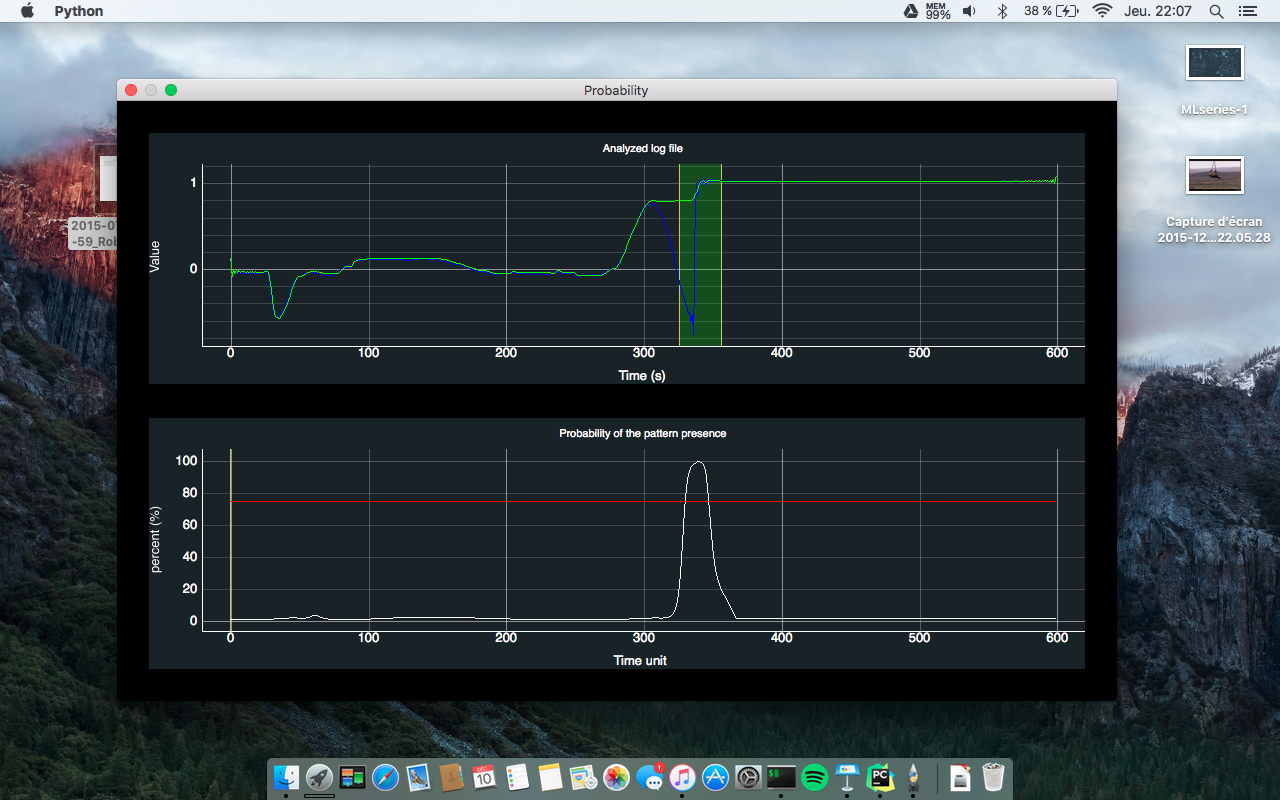
\includegraphics[height=7cm]{images/proba_visu.png}
	\caption[Interface graphique du probability visualizator]{Interface graphique du probability visualizator.}
	\label{fig:Interface graphique du probability visualizator}
\end{figure}

\subsection{Control panel}
\label{Industrialisation du produit: Outils graphiques: Control panel}
Le control panel permet d'obtenir un certain nombre d'informations quant à la qualité de la base de données d'exemple utilisée pour créer une nouvelle couche \emph{root cause}, ainsi que sur les performances de l'algorithme d'apprentissage automatique. La plupart de ces informations sont déterminées grâce aux outils soumis en partie \ref{Automatisation du processus d'investigation: Performances de la solution}. L'IHM est composé de trois parties.
\begin{description}
	\item [Data set features] (encadré vert sur la figure \ref{fig:Interface graphique du control pattern}) fournit un ensemble d'informations sur la base de données d'exemples utilisée pour l'entraînement de l'algorithme d'apprentissage automatique. 
	\item [Training panel features ](encadré rouge sur la figure \ref{fig:Interface graphique du control pattern} nous livre des informations sur  l'algorithme d'apprentissage automatique de la couche root cause analysée (e.g. valeur des paramètres, matrice de confusion, précision, etc). Ces données sont pour la plupart relatives aux explications fournies en partie \ref{Automatisation du processus d'investigation: Performances de la solution}.
	\item [Training panel ](encadré bleu sur la figure \ref{fig:Interface graphique du control pattern}) permet d'analyser les courbes d'apprentissage (c.f. partie \ref{Industrialisation du produit: Performances de la solution:Courbes d'apprentissage}) et les courbes de validation (c.f. partie \ref{Industrialisation du produit: Performances de la solution:Optimisation des paramètres du SVM})
\end{description}

\begin{figure}[H]
	\centering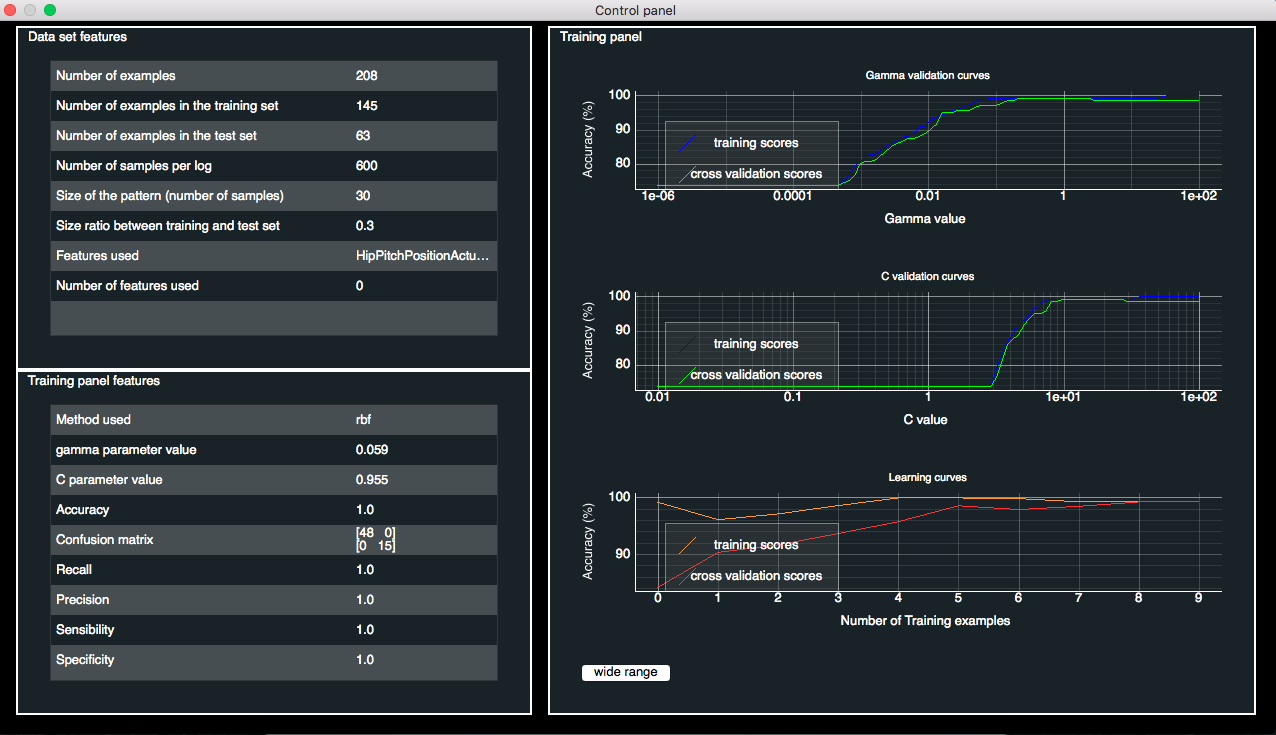
\includegraphics[height=7cm]{images/control_panel.png}
	\caption[Interface graphique du control pattern]{Interface graphique du control pattern.}
	\label{fig:Interface graphique du control pattern}
\end{figure}

\section{Utilisation suggérée des outils}
\label{Industrialisation du produit: Utilisation suggérée des outils}
On propose dans cette partie un exemple d'utilisation de l'API et des interfaces graphiques. Cette solution a été mise en place dans le cadre du stage afin de proposer un script qui permet d'ores et déjà de gérer la base de donnée, de créer de nouvelles couches \emph{root cause} et d'investiguer des fichiers logs. On s'appuie sur l'utilisation de la libraire python \emph{npyscreen} \cite{Npyscreen} qui permet de réaliser des interfaces utilisateurs simples, directement dans le terminal.
\newline

On s'intéressera ici au problème de frottement des freins de la hanche, qui entraîne la chute du robot durant le Filtering Test. Sa résolution passe donc par trois étapes: 
\begin{enumerate}
	\item Créer une nouvelle couche \emph{error name} : la couche "chute du robot". 
	\item Créer un nouvelle couche \emph{root cause} liée à la couche \emph{error name} "chute du robot" : la couche "frottement des freins de la hanche". Cela signifie que l'on va entraîner un nouvel algorithme à détecter le motif caractéristique de cette \emph{root cause}. 
	\item vérifier les performances de la nouvelle couche \emph{root cause} créée via le Control Panel.
	\item Investiguer un fichier log. 
\end{enumerate}

\subsection{Menu principal}
\label{Industrialisation du produit: Utilisation suggérée des outils: Menu principal}
Le menu principal (c.f. figure ) permet d'ouvrir 5 sous-menus qui permettent respectivement:
\begin{itemize}
	\item Créer une nouvelle couche \emph{error name} et l'ajouter à la base de données.
	\item Créer une nouvelle couche \emph{root cause}, la lier à une couche \emph{error name} et l'ajouter à la base de données.
	\item Investiguer un fichier log
	\item Mettre à jour une \emph{root cause}
	\item Ouvrir le control panel
\end{itemize}

\begin{figure}[H]
	\centering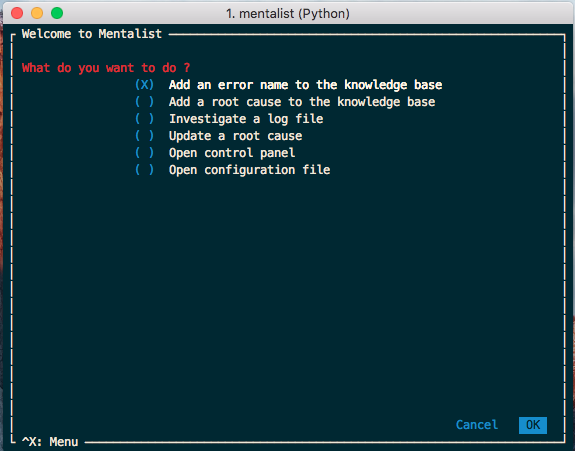
\includegraphics[height=7cm]{images/main_menu.png}
	\caption[Menu principal]{Menu principal.}
	\label{fig:Menu principal}
\end{figure} 

\subsection{Nouvelle error name}
\label{Industrialisation du produit: Utilisation suggérée des outils: Nouvelle error name}
Le menu "Add an error name to the knowledge base" (c.f. figure 	\ref{fig:Menu principal}) permet d'ajouter une couche \emph{error name} dans la base de données. \\
Il suffit pour cela d'indiquer le nom de la couche \emph{error name} que l'on souhaite créer: dans notre cas, on l'appellera \textbf{fall down}. Celle-ci ne contient à sa création aucune \emph{root cause}.

\subsection{Nouvelle root cause}
\label{Industrialisation du produit: Utilisation suggérée des outils: Nouvelle root cause}
Le menu "Add a root cause to the knowledge base" (c.f. figure \ref{fig:Menu principal}) permet de créer une nouvelle \emph{root cause} (i.e. entraîner un nouvel algorithme d'apprentissage à reconnaitre une \emph{root cause}), à la lier à une couche \emph{error name}, et à l'ajouter à la base données. \\
Pour cela, on suit le processus suivant (c.f. figure \ref{fig: Nouvelle root cause}) : 
\begin{enumerate}
	\item On sélectionne l'\emph{error name} à laquelle on souhaite lier cette nouvelle \emph{root cause}. On indique ensuite son nom. Dans le cas de la \emph{root cause} "frottement des freins de la hanche", on la lie à l'\emph{error name} "fall down" et on l'appelle "frottement des freins de la hanche". 
	\item On sélectionne la/les feature(s) liée(s) à la \emph{root cause}. Dans le cas de la \emph{root cause} du "frottement des freins de la hanche", on sélectionne les clés HipPitchPositionSensorValue, HipPitchPositionActuatorValue, respectivement les valeurs du senseur et de l'actuateur de la hanche. 
	\item On utilise le Pattern Selector (c.f. partie \ref{Industrialisation du produit: Outils graphiques: Pattern selection}) pour sélectionner les motifs caractéristiques de la \emph{root cause} que l'on étudie. Dans notre cas, il s'agit du moment où le senseur ne suit plus actuateur. On répète cette manipulation pour chaque exemple de la base de données.
\end{enumerate}

\begin{figure}[H]
	\centering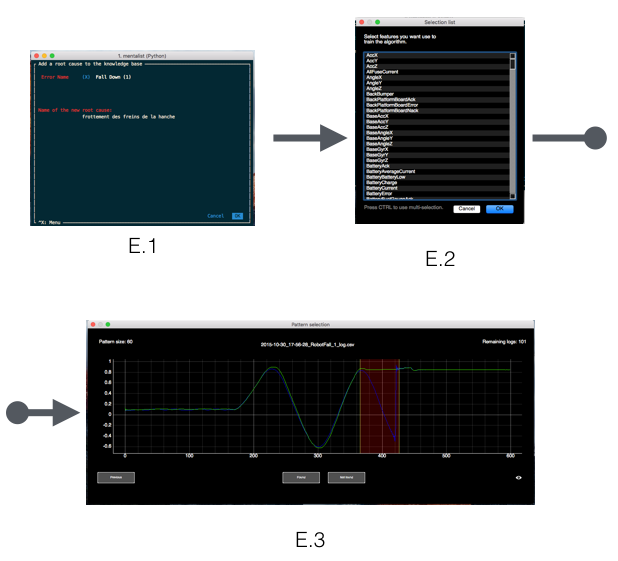
\includegraphics[width=10cm]{images/add_root_menu.png}
	\caption[Nouvelle root cause]{Nouvelle root cause.}
	\label{fig: Nouvelle root cause}
\end{figure} 


\subsection{Investiguer un fichier log}
\label{Industrialisation du produit: Utilisation suggérée des outils: Investiguer}
Le menu "Investigate a log file" (c.f. figure \ref{fig:Menu principal}) permet de réaliser une investigation sur un fichier log, i.e. trouver la root cause ayant entraîné l'apparition de l'error name durant le Filtering Test. Pour cela, on suit le processus suivant (c.f. figure \ref{fig: Investigation d'un fichier log}) : 
\begin{enumerate}
	\item On commence par indiquer au script le chemin vers le fichier log. On sélectionne ensuite l'error name que l'on souhaite investiguer, parmi la liste des errors name connues (i.e. présentes dans la base de données).
	\item Le programme nous affiche Probability Visualizator (c.f. partie \ref{Industrialisation du produit: Outils graphiques: Probability Visualization})
	\item Une fois le Probability Visualizator fermé, le script nous indique la root cause trouvée dans le fichier log. 
\end{enumerate}

\begin{figure}[H]
	\centering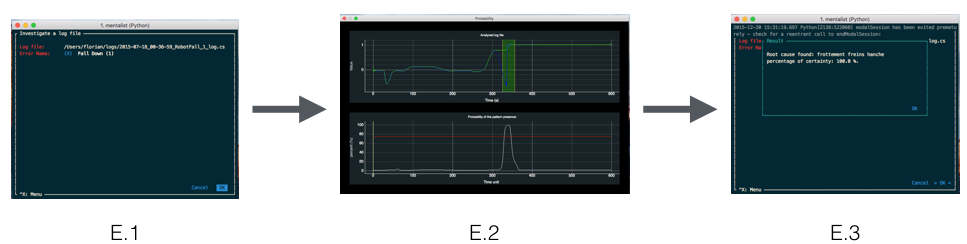
\includegraphics[height=4cm]{images/invest_menu.png}
	\caption[Investigation d'un fichier log]{Investigation d'un fichier log.}
	\label{fig: Investigation d'un fichier log}
\end{figure} 

\subsection{Analyse des performances d'une  root cause}
\label{Industrialisation du produit: Utilisation suggérée des outils: Analyse des performances d'une  root cause}
Le menu "Open control panel" (c.f. figure \ref{fig:Menu principal}) permet de sélectionner une root cause liée à une error name et d'en afficher le control panel afin d'obtenir des informations sur la qualité des exemples utilisés pour entraîner l'algorithme d'apprentissage automatique ainsi que ses performances. Pour cela, on suit le processus suivant (c.f. figure \ref{fig: Analyse des performances d'une couche root cause}) : 
\begin{enumerate}
	\item On sélectionne dans l'arborescence des errors name et des root cause qui leurs sont liées la root cause que l'on souhaite étudier.
	\item Le control panel s'affiche (c.f. partie \ref{Industrialisation du produit: Outils graphiques: Control panel})
\end{enumerate}

\begin{figure}[H]
	\centering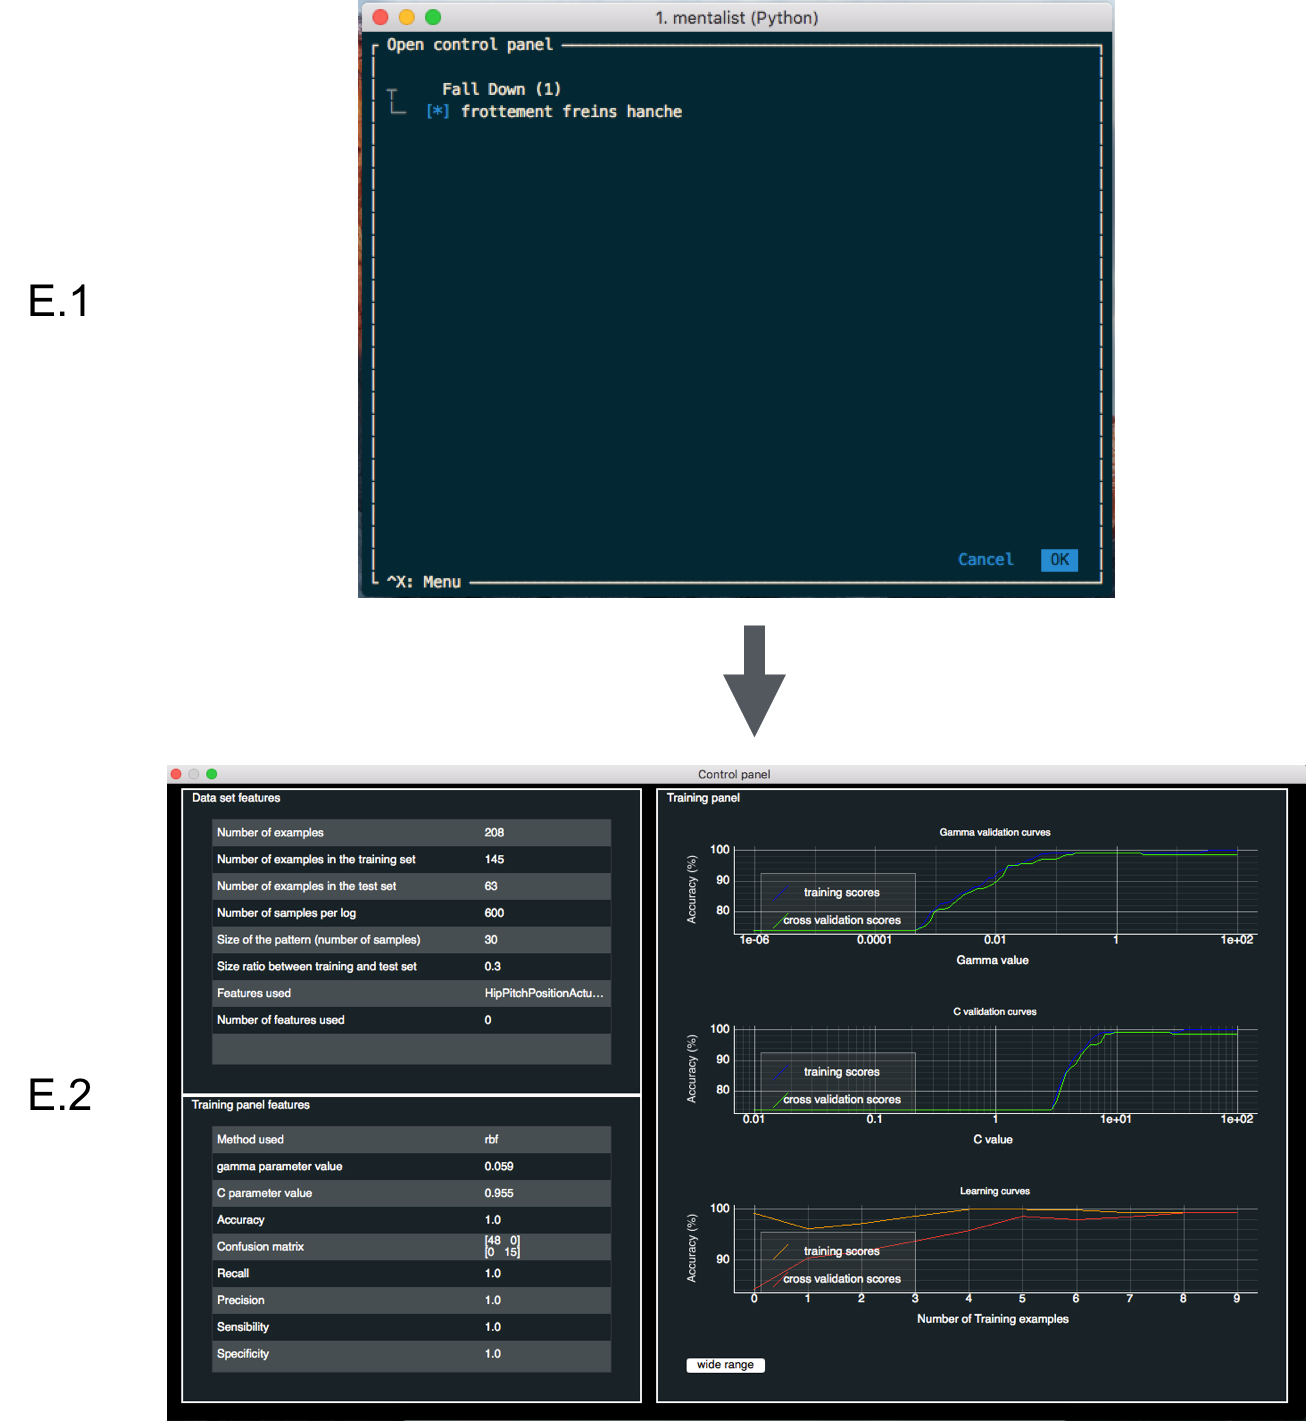
\includegraphics[height=5.5cm]{images/perf_menu.png}
	\caption[Analyse des performances d'une couche root cause]{Analyse des performances d'une couche root cause.}
	\label{fig: Analyse des performances d'une couche root cause}
\end{figure} 


\subsection{Mise à jour d'une root cause}
\label{Industrialisation du produit: Utilisation suggérée des outils: Mise à jour d'une root cause}
Le menu "Update a root cause"  (c.f. figure \ref{fig:Menu principal}) permet d'ajouter des exemples à la base de données d'exemples d'une root cause déjà connue (i.e. enregistrée dans la base de données) et d'entrainer de nouveau l'algorithme d'apprentissage afin d'en améliorer les performances. Pour cela, on suit le processus suivant (c.f. figure \ref{fig: Analyse des performances d'une couche root cause}) : 
\begin{enumerate}
	\item On sélectionne dans l'arborescence des errors name et des root cause qui leurs sont liées la root cause que l'on souhaite mettre à jour.
	\item On sélectionne les motifs caractéristiques de la root cause dans les exemples ajoutés.
\end{enumerate}

\begin{figure}[H]
	\centering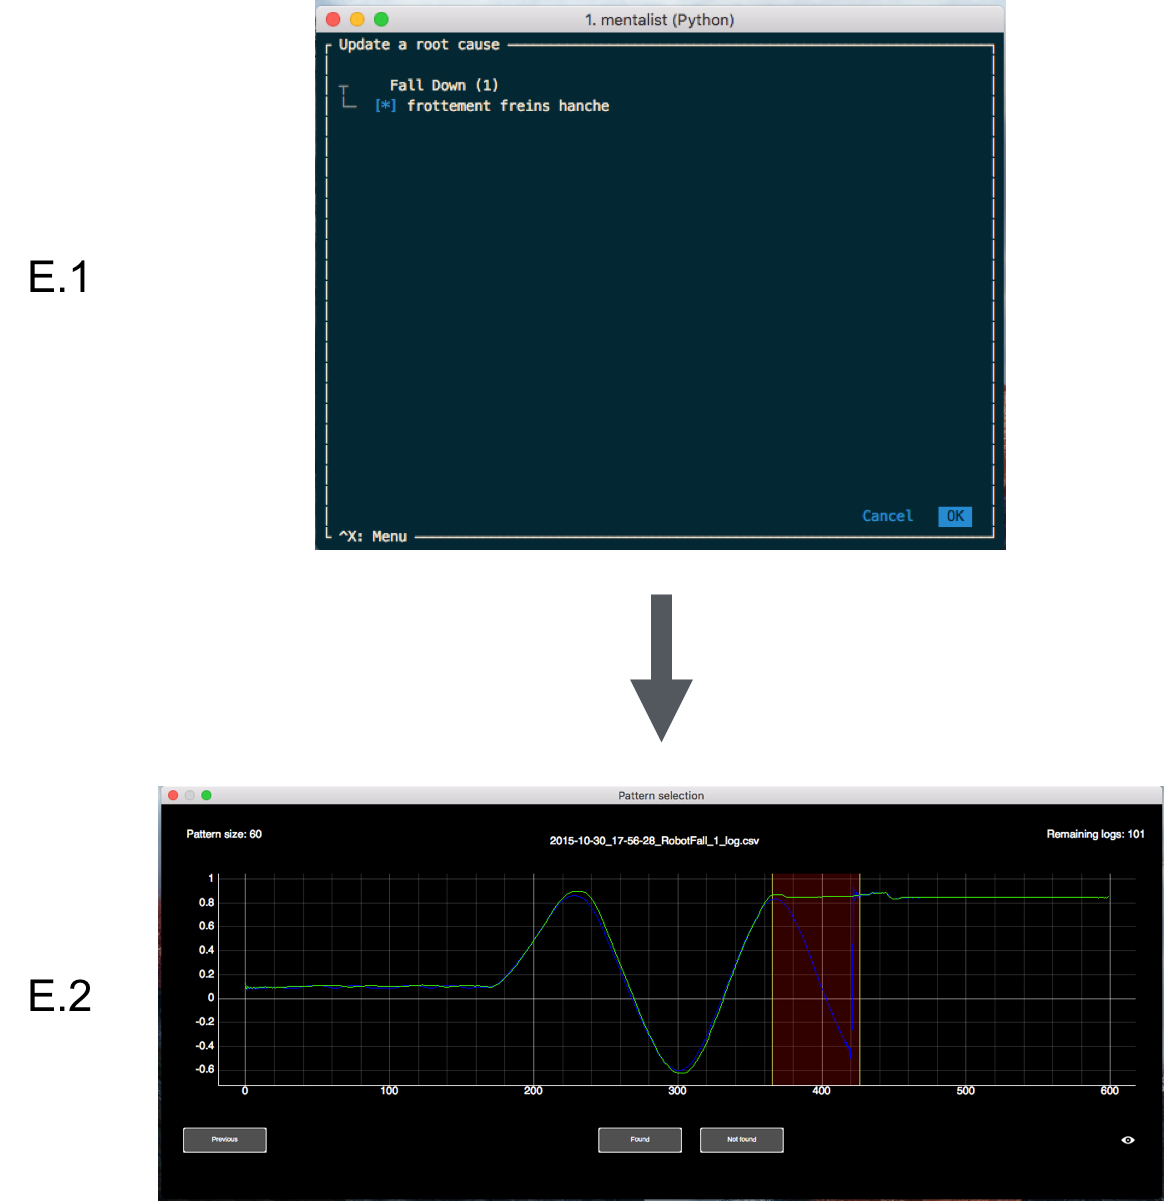
\includegraphics[height=5cm]{images/update_menu.png}
	\caption[Mise à jour d'une root cause]{Mise à jour d'une root cause.}
	\label{fig: Mise à jour d'une root cause}
\end{figure} 


\section{Dimensionnement de la solution}
\label{Industrialisation du produit: Dimensionnement de la solution}
Contrairement à l'étude réalisée en partie \ref{Automatisation du processus d'investigation: Performances de la solution}, on désire mesurer ici non pas uniquement la performance de l'algorithme, mais également l'influence du facteur humain sur celle-ci. On s'intéresse notamment à l'impact qu'à l'évolution de la taille de la région mobile du Pattern selector (c.f. partie \ref{Industrialisation du produit: Outils graphiques: Pattern selection}), qui permet de sélectionner les échantillons du motif caractéristique d'une root cause. En effet, cette variable dépend de la forme du motif, mais également de l'appréciation de l'utilisateur (quand commence le motif, quand se termine-t-il ?). \\
Afin de quantifier cette dimension, on réalise plusieurs fois la création de la couche root cause du "frottement des freins de la hanche" en augmentant à chaque fois la taille de la région de sélection. On prélève la précision à chaque itération. On affiche la courbe d'évolution de la précision de l'algorithme d'apprentissage automatique, en fonction de la taille de la région de sélection en figure \ref{fig: Evolution de la précision de l'algorithme en fonction de la taille de la région de sélection}

\begin{figure}[H]
	\centering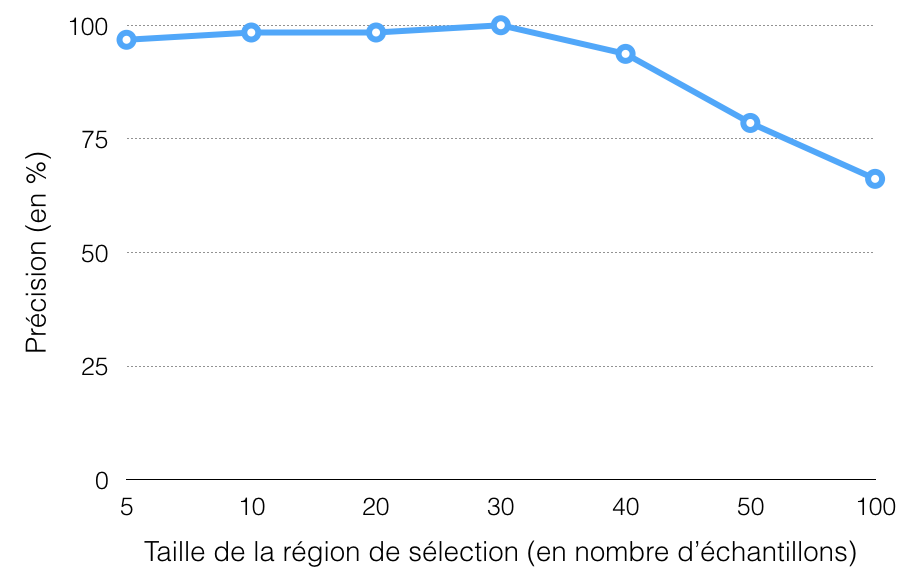
\includegraphics[height=8cm]{images/precision_taille.png}
	\caption[Evolution de la précision de l'algorithme en fonction de la taille de la région de sélection]{Évolution de la précision de l'algorithme en fonction de la taille de la région de sélection.  On observe que entre une taille de 10 et 30 échantillons, la précision de l'algorithme augmente légèrement. A partir de 30 échantillons, la précision de l'algorithme diminue.}
	\label{fig: Evolution de la précision de l'algorithme en fonction de la taille de la région de sélection}
\end{figure} 

Au regard des valeurs obtenues, on en déduit que l'algorithme est plus performant lorsque la région de sélection est petite. Or, le but est également de sélectionner le plus précisément possible le motif caractéristique d'une root cause. Il faut donc jauger chaque situation au cas par cas,  en gardant en tête ces deux contraintes. Par exemple, si on souhaite apprendre notre algorithme à reconnaitre une région ayant une taille de 50 échantillons, il sera peut-être plus opportun d'apprendre l'algorithme à reconnaitre seulement une partie du motif (de 30 échantillons environ).
chapter{Conclusion}
\label{Conclusion}
\thispagestyle{fancy}
\bibliographystyle{unsrt}
\bibliography{biblio}
\include {annexes}
\end{document}
